\documentclass{article}
\usepackage{tikz}
\usepackage{xcolor}
\definecolor{vizDefault}{HTML}{9CA3AF}
\definecolor{vizComparing}{HTML}{FFA768}
\definecolor{vizSwapping}{HTML}{E14B53}
\definecolor{vizSorted}{HTML}{5BF15D}
\definecolor{vizActive}{HTML}{629BF8}
\definecolor{vizExplored}{HTML}{7C4FDB}
\definecolor{vizUpdated}{HTML}{E0A400}
\usetikzlibrary{matrix}
\usepackage[margin=1in]{geometry}
\begin{document}
% --- Frame 0 ---
\begin{center}\LARGE\textbf{Dijkstra}\\[6mm]\end{center}
\begin{center}
\begin{center}\textbf{Log}\\[1.75mm]\end{center}
\begin{tikzpicture}
  \filldraw[fill=white!0, draw=none] (0,0) rectangle (10cm, -0.25cm);
  \node[anchor=north, align=center, text=black] at (5cm,0) {\texttt{Initial state}};
\end{tikzpicture}
\end{center}
\noindent\rule{\linewidth}{0.3pt}
\begin{center}
\begin{center}\textbf{Graph}\\[2mm]\end{center}
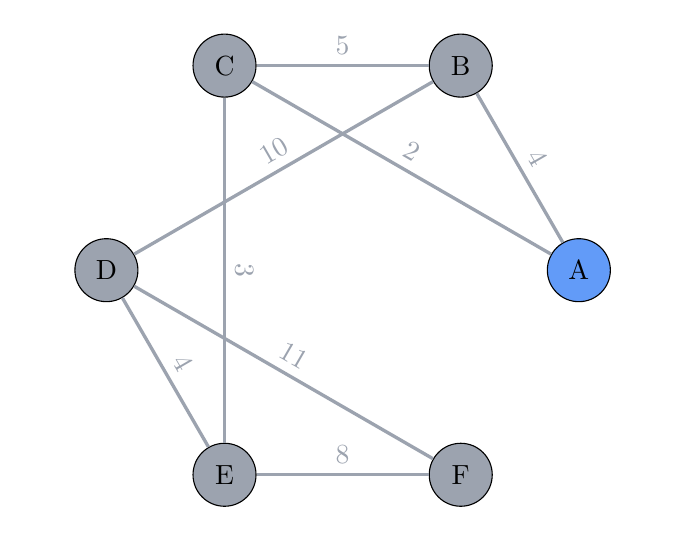
\begin{tikzpicture}
  \filldraw[fill=white!0, draw=none] (-4cm,0) rectangle (4cm, -3cm);
  \node[circle, draw, minimum size=8mm, fill=vizActive] (A) at (0.0:3cm) {A};
  \node[circle, draw, minimum size=8mm, fill=vizDefault] (B) at (60.0:3cm) {B};
  \node[circle, draw, minimum size=8mm, fill=vizDefault] (C) at (120.0:3cm) {C};
  \node[circle, draw, minimum size=8mm, fill=vizDefault] (D) at (180.0:3cm) {D};
  \node[circle, draw, minimum size=8mm, fill=vizDefault] (E) at (240.0:3cm) {E};
  \node[circle, draw, minimum size=8mm, fill=vizDefault] (F) at (300.0:3cm) {F};
  \draw[vizDefault, line width=1.2pt] (A) -- node[midway, sloped, above] {4} (B);
  \draw[vizDefault, line width=1.2pt] (A) -- node[midway, sloped, above] {2} (C);
  \draw[vizDefault, line width=1.2pt] (B) -- node[midway, sloped, above] {5} (C);
  \draw[vizDefault, line width=1.2pt] (B) -- node[midway, sloped, above] {10} (D);
  \draw[vizDefault, line width=1.2pt] (C) -- node[midway, sloped, above] {3} (E);
  \draw[vizDefault, line width=1.2pt] (D) -- node[midway, sloped, above] {11} (F);
  \draw[vizDefault, line width=1.2pt] (E) -- node[midway, sloped, above] {4} (D);
  \draw[vizDefault, line width=1.2pt] (E) -- node[midway, sloped, above] {8} (F);
\end{tikzpicture}
\end{center}
\noindent\rule{\linewidth}{0.3pt}
\begin{center}
\begin{center}\textbf{Open Set}\\[1.75mm]\end{center}

\begin{tikzpicture}
  \filldraw[fill=white!0, draw=none] (0cm,0cm) rectangle (0.8cm, -1cm);
  \filldraw[fill=vizDefault] (0cm,-0.8cm) rectangle (0.8cm,0cm);
  \node at (0.4cm,-0.4cm) {A};
\end{tikzpicture}
\end{center}
\noindent\rule{\linewidth}{0.3pt}
\begin{center}
\begin{center}\textbf{Closed Set}\\[1.75mm]\end{center}
\begin{tikzpicture}
  \filldraw[fill=white!0, draw=none] (0cm,0cm) rectangle (0cm, -1cm);
\end{tikzpicture}
\end{center}
\noindent\rule{\linewidth}{0.3pt}
\begin{center}
\begin{center}\textbf{Node Costs}\\[1.75mm]\end{center}
\begin{tikzpicture}
  \filldraw[fill=white!0, draw=none] (0cm,0) rectangle (0.5cm,3.5cm);
  \node[above] at (0.25cm,0cm) {0};
  \node[below] at (0.25cm,0) {A};
  \filldraw[fill=white!0, draw=none] (0.7cm,0) rectangle (1.2cm,3.5cm);
  \node[above] at (0.95cm,0cm) {0};
  \node[below] at (0.95cm,0) {B};
  \filldraw[fill=white!0, draw=none] (1.4cm,0) rectangle (1.9cm,3.5cm);
  \node[above] at (1.65cm,0cm) {0};
  \node[below] at (1.65cm,0) {C};
  \filldraw[fill=white!0, draw=none] (2.0999999999999996cm,0) rectangle (2.5999999999999996cm,3.5cm);
  \node[above] at (2.3499999999999996cm,0cm) {0};
  \node[below] at (2.3499999999999996cm,0) {D};
  \filldraw[fill=white!0, draw=none] (2.8cm,0) rectangle (3.3cm,3.5cm);
  \node[above] at (3.05cm,0cm) {0};
  \node[below] at (3.05cm,0) {E};
  \filldraw[fill=white!0, draw=none] (3.5cm,0) rectangle (4cm,3.5cm);
  \node[above] at (3.75cm,0cm) {0};
  \node[below] at (3.75cm,0) {F};
\end{tikzpicture}
\end{center}
\newpage
% --- Frame 1 ---
\begin{center}\LARGE\textbf{Dijkstra}\\[6mm]\end{center}
\begin{center}
\begin{center}\textbf{Log}\\[1.75mm]\end{center}

\begin{tikzpicture}
  \filldraw[fill=white!0, draw=none] (0,0) rectangle (10cm, -0.25cm);
  \node[anchor=north, align=center, text=black] at (5cm,0) {\texttt{Sorting the open set so the lowest-cost node comes first.}};
\end{tikzpicture}
\end{center}
\noindent\rule{\linewidth}{0.3pt}
\begin{center}
\begin{center}\textbf{Graph}\\[2mm]\end{center}
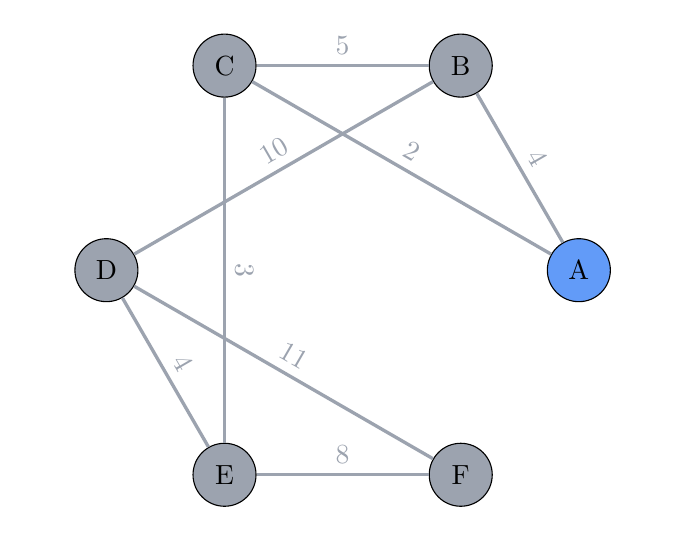
\begin{tikzpicture}
  \filldraw[fill=white!0, draw=none] (-4cm,0) rectangle (4cm, -3cm);
  \node[circle, draw, minimum size=8mm, fill=vizActive] (A) at (0.0:3cm) {A};
  \node[circle, draw, minimum size=8mm, fill=vizDefault] (B) at (60.0:3cm) {B};
  \node[circle, draw, minimum size=8mm, fill=vizDefault] (C) at (120.0:3cm) {C};
  \node[circle, draw, minimum size=8mm, fill=vizDefault] (D) at (180.0:3cm) {D};
  \node[circle, draw, minimum size=8mm, fill=vizDefault] (E) at (240.0:3cm) {E};
  \node[circle, draw, minimum size=8mm, fill=vizDefault] (F) at (300.0:3cm) {F};
  \draw[vizDefault, line width=1.2pt] (A) -- node[midway, sloped, above] {4} (B);
  \draw[vizDefault, line width=1.2pt] (A) -- node[midway, sloped, above] {2} (C);
  \draw[vizDefault, line width=1.2pt] (B) -- node[midway, sloped, above] {5} (C);
  \draw[vizDefault, line width=1.2pt] (B) -- node[midway, sloped, above] {10} (D);
  \draw[vizDefault, line width=1.2pt] (C) -- node[midway, sloped, above] {3} (E);
  \draw[vizDefault, line width=1.2pt] (D) -- node[midway, sloped, above] {11} (F);
  \draw[vizDefault, line width=1.2pt] (E) -- node[midway, sloped, above] {4} (D);
  \draw[vizDefault, line width=1.2pt] (E) -- node[midway, sloped, above] {8} (F);
\end{tikzpicture}
\end{center}
\noindent\rule{\linewidth}{0.3pt}
\begin{center}
\begin{center}\textbf{Open Set}\\[1.75mm]\end{center}
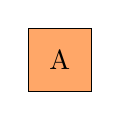
\begin{tikzpicture}
  \filldraw[fill=white!0, draw=none] (0cm,0cm) rectangle (0.8cm, -1cm);
  \filldraw[fill=vizComparing] (0cm,-0.8cm) rectangle (0.8cm,0cm);
  \node at (0.4cm,-0.4cm) {A};
\end{tikzpicture}
\end{center}
\noindent\rule{\linewidth}{0.3pt}
\begin{center}
\begin{center}\textbf{Closed Set}\\[1.75mm]\end{center}
\begin{tikzpicture}
  \filldraw[fill=white!0, draw=none] (0cm,0cm) rectangle (0cm, -1cm);
\end{tikzpicture}
\end{center}
\noindent\rule{\linewidth}{0.3pt}
\begin{center}
\begin{center}\textbf{Node Costs}\\[1.75mm]\end{center}
\begin{tikzpicture}
  \filldraw[fill=white!0, draw=none] (0cm,0) rectangle (0.5cm,3.5cm);
  \node[above] at (0.25cm,0cm) {0};
  \node[below] at (0.25cm,0) {A};
  \filldraw[fill=white!0, draw=none] (0.7cm,0) rectangle (1.2cm,3.5cm);
  \node[above] at (0.95cm,0cm) {0};
  \node[below] at (0.95cm,0) {B};
  \filldraw[fill=white!0, draw=none] (1.4cm,0) rectangle (1.9cm,3.5cm);
  \node[above] at (1.65cm,0cm) {0};
  \node[below] at (1.65cm,0) {C};
  \filldraw[fill=white!0, draw=none] (2.0999999999999996cm,0) rectangle (2.5999999999999996cm,3.5cm);
  \node[above] at (2.3499999999999996cm,0cm) {0};
  \node[below] at (2.3499999999999996cm,0) {D};
  \filldraw[fill=white!0, draw=none] (2.8cm,0) rectangle (3.3cm,3.5cm);
  \node[above] at (3.05cm,0cm) {0};
  \node[below] at (3.05cm,0) {E};
  \filldraw[fill=white!0, draw=none] (3.5cm,0) rectangle (4cm,3.5cm);
  \node[above] at (3.75cm,0cm) {0};
  \node[below] at (3.75cm,0) {F};
\end{tikzpicture}
\end{center}
\newpage
% --- Frame 2 ---
\begin{center}\LARGE\textbf{Dijkstra}\\[6mm]\end{center}
\begin{center}
\begin{center}\textbf{Log}\\[1.75mm]\end{center}

\begin{tikzpicture}
  \filldraw[fill=white!0, draw=none] (0,0) rectangle (10cm, -0.25cm);
  \node[anchor=north, align=center, text=black] at (5cm,0) {\texttt{Grabbing the lowest-cost node from the open set.}};
\end{tikzpicture}
\end{center}
\noindent\rule{\linewidth}{0.3pt}
\begin{center}
\begin{center}\textbf{Graph}\\[2mm]\end{center}
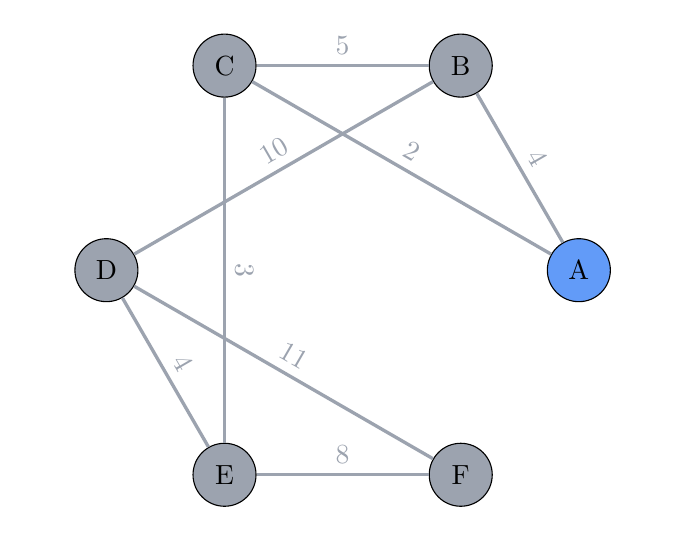
\begin{tikzpicture}
  \filldraw[fill=white!0, draw=none] (-4cm,0) rectangle (4cm, -3cm);
  \node[circle, draw, minimum size=8mm, fill=vizActive] (A) at (0.0:3cm) {A};
  \node[circle, draw, minimum size=8mm, fill=vizDefault] (B) at (60.0:3cm) {B};
  \node[circle, draw, minimum size=8mm, fill=vizDefault] (C) at (120.0:3cm) {C};
  \node[circle, draw, minimum size=8mm, fill=vizDefault] (D) at (180.0:3cm) {D};
  \node[circle, draw, minimum size=8mm, fill=vizDefault] (E) at (240.0:3cm) {E};
  \node[circle, draw, minimum size=8mm, fill=vizDefault] (F) at (300.0:3cm) {F};
  \draw[vizDefault, line width=1.2pt] (A) -- node[midway, sloped, above] {4} (B);
  \draw[vizDefault, line width=1.2pt] (A) -- node[midway, sloped, above] {2} (C);
  \draw[vizDefault, line width=1.2pt] (B) -- node[midway, sloped, above] {5} (C);
  \draw[vizDefault, line width=1.2pt] (B) -- node[midway, sloped, above] {10} (D);
  \draw[vizDefault, line width=1.2pt] (C) -- node[midway, sloped, above] {3} (E);
  \draw[vizDefault, line width=1.2pt] (D) -- node[midway, sloped, above] {11} (F);
  \draw[vizDefault, line width=1.2pt] (E) -- node[midway, sloped, above] {4} (D);
  \draw[vizDefault, line width=1.2pt] (E) -- node[midway, sloped, above] {8} (F);
\end{tikzpicture}
\end{center}
\noindent\rule{\linewidth}{0.3pt}
\begin{center}
\begin{center}\textbf{Open Set}\\[1.75mm]\end{center}

\begin{tikzpicture}
  \filldraw[fill=white!0, draw=none] (0cm,0cm) rectangle (0.8cm, -1cm);
  \filldraw[fill=vizSwapping] (0cm,-0.8cm) rectangle (0.8cm,0cm);
  \node at (0.4cm,-0.4cm) {A};
\end{tikzpicture}
\end{center}
\noindent\rule{\linewidth}{0.3pt}
\begin{center}
\begin{center}\textbf{Closed Set}\\[1.75mm]\end{center}
\begin{tikzpicture}
  \filldraw[fill=white!0, draw=none] (0cm,0cm) rectangle (0cm, -1cm);
\end{tikzpicture}
\end{center}
\noindent\rule{\linewidth}{0.3pt}
\begin{center}
\begin{center}\textbf{Node Costs}\\[1.75mm]\end{center}
\begin{tikzpicture}
  \filldraw[fill=white!0, draw=none] (0cm,0) rectangle (0.5cm,3.5cm);
  \node[above] at (0.25cm,0cm) {0};
  \node[below] at (0.25cm,0) {A};
  \filldraw[fill=white!0, draw=none] (0.7cm,0) rectangle (1.2cm,3.5cm);
  \node[above] at (0.95cm,0cm) {0};
  \node[below] at (0.95cm,0) {B};
  \filldraw[fill=white!0, draw=none] (1.4cm,0) rectangle (1.9cm,3.5cm);
  \node[above] at (1.65cm,0cm) {0};
  \node[below] at (1.65cm,0) {C};
  \filldraw[fill=white!0, draw=none] (2.0999999999999996cm,0) rectangle (2.5999999999999996cm,3.5cm);
  \node[above] at (2.3499999999999996cm,0cm) {0};
  \node[below] at (2.3499999999999996cm,0) {D};
  \filldraw[fill=white!0, draw=none] (2.8cm,0) rectangle (3.3cm,3.5cm);
  \node[above] at (3.05cm,0cm) {0};
  \node[below] at (3.05cm,0) {E};
  \filldraw[fill=white!0, draw=none] (3.5cm,0) rectangle (4cm,3.5cm);
  \node[above] at (3.75cm,0cm) {0};
  \node[below] at (3.75cm,0) {F};
\end{tikzpicture}
\end{center}
\newpage
% --- Frame 3 ---
\begin{center}\LARGE\textbf{Dijkstra}\\[6mm]\end{center}
\begin{center}
\begin{center}\textbf{Log}\\[1.75mm]\end{center}

\begin{tikzpicture}
  \filldraw[fill=white!0, draw=none] (0,0) rectangle (10cm, -0.25cm);
  \node[anchor=north, align=center, text=black] at (5cm,0) {\texttt{Visiting node A and moving it to the closed set.}};
\end{tikzpicture}
\end{center}
\noindent\rule{\linewidth}{0.3pt}
\begin{center}
\begin{center}\textbf{Graph}\\[2mm]\end{center}
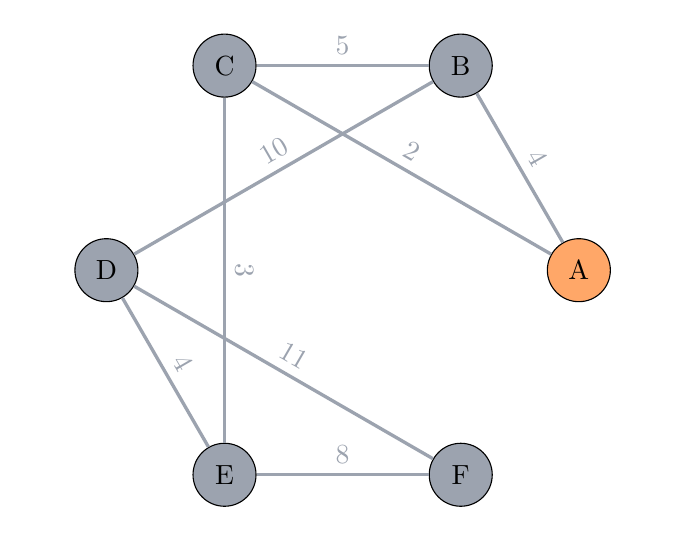
\begin{tikzpicture}
  \filldraw[fill=white!0, draw=none] (-4cm,0) rectangle (4cm, -3cm);
  \node[circle, draw, minimum size=8mm, fill=vizComparing] (A) at (0.0:3cm) {A};
  \node[circle, draw, minimum size=8mm, fill=vizDefault] (B) at (60.0:3cm) {B};
  \node[circle, draw, minimum size=8mm, fill=vizDefault] (C) at (120.0:3cm) {C};
  \node[circle, draw, minimum size=8mm, fill=vizDefault] (D) at (180.0:3cm) {D};
  \node[circle, draw, minimum size=8mm, fill=vizDefault] (E) at (240.0:3cm) {E};
  \node[circle, draw, minimum size=8mm, fill=vizDefault] (F) at (300.0:3cm) {F};
  \draw[vizDefault, line width=1.2pt] (A) -- node[midway, sloped, above] {4} (B);
  \draw[vizDefault, line width=1.2pt] (A) -- node[midway, sloped, above] {2} (C);
  \draw[vizDefault, line width=1.2pt] (B) -- node[midway, sloped, above] {5} (C);
  \draw[vizDefault, line width=1.2pt] (B) -- node[midway, sloped, above] {10} (D);
  \draw[vizDefault, line width=1.2pt] (C) -- node[midway, sloped, above] {3} (E);
  \draw[vizDefault, line width=1.2pt] (D) -- node[midway, sloped, above] {11} (F);
  \draw[vizDefault, line width=1.2pt] (E) -- node[midway, sloped, above] {4} (D);
  \draw[vizDefault, line width=1.2pt] (E) -- node[midway, sloped, above] {8} (F);
\end{tikzpicture}
\end{center}
\noindent\rule{\linewidth}{0.3pt}
\begin{center}
\begin{center}\textbf{Open Set}\\[1.75mm]\end{center}
\begin{tikzpicture}
  \filldraw[fill=white!0, draw=none] (0cm,0cm) rectangle (0cm, -1cm);
\end{tikzpicture}
\end{center}
\noindent\rule{\linewidth}{0.3pt}
\begin{center}
\begin{center}\textbf{Closed Set}\\[1.75mm]\end{center}

\begin{tikzpicture}
  \filldraw[fill=white!0, draw=none] (0cm,0cm) rectangle (0.8cm, -1cm);
  \filldraw[fill=vizActive] (0cm,-0.8cm) rectangle (0.8cm,0cm);
  \node at (0.4cm,-0.4cm) {A};
\end{tikzpicture}
\end{center}
\noindent\rule{\linewidth}{0.3pt}
\begin{center}
\begin{center}\textbf{Node Costs}\\[1.75mm]\end{center}
\begin{tikzpicture}
  \filldraw[fill=white!0, draw=none] (0cm,0) rectangle (0.5cm,3.5cm);
  \node[above] at (0.25cm,0cm) {0};
  \node[below] at (0.25cm,0) {A};
  \filldraw[fill=white!0, draw=none] (0.7cm,0) rectangle (1.2cm,3.5cm);
  \node[above] at (0.95cm,0cm) {0};
  \node[below] at (0.95cm,0) {B};
  \filldraw[fill=white!0, draw=none] (1.4cm,0) rectangle (1.9cm,3.5cm);
  \node[above] at (1.65cm,0cm) {0};
  \node[below] at (1.65cm,0) {C};
  \filldraw[fill=white!0, draw=none] (2.0999999999999996cm,0) rectangle (2.5999999999999996cm,3.5cm);
  \node[above] at (2.3499999999999996cm,0cm) {0};
  \node[below] at (2.3499999999999996cm,0) {D};
  \filldraw[fill=white!0, draw=none] (2.8cm,0) rectangle (3.3cm,3.5cm);
  \node[above] at (3.05cm,0cm) {0};
  \node[below] at (3.05cm,0) {E};
  \filldraw[fill=white!0, draw=none] (3.5cm,0) rectangle (4cm,3.5cm);
  \node[above] at (3.75cm,0cm) {0};
  \node[below] at (3.75cm,0) {F};
\end{tikzpicture}
\end{center}
\newpage
% --- Frame 4 ---
\begin{center}\LARGE\textbf{Dijkstra}\\[6mm]\end{center}
\begin{center}
\begin{center}\textbf{Log}\\[1.75mm]\end{center}

\begin{tikzpicture}
  \filldraw[fill=white!0, draw=none] (0,0) rectangle (10cm, -0.25cm);
  \node[anchor=north, align=center, text=black] at (5cm,0) {\texttt{Looking at neighbor B — is going through A cheaper than what we already know?}};
\end{tikzpicture}
\end{center}
\noindent\rule{\linewidth}{0.3pt}
\begin{center}
\begin{center}\textbf{Graph}\\[2mm]\end{center}
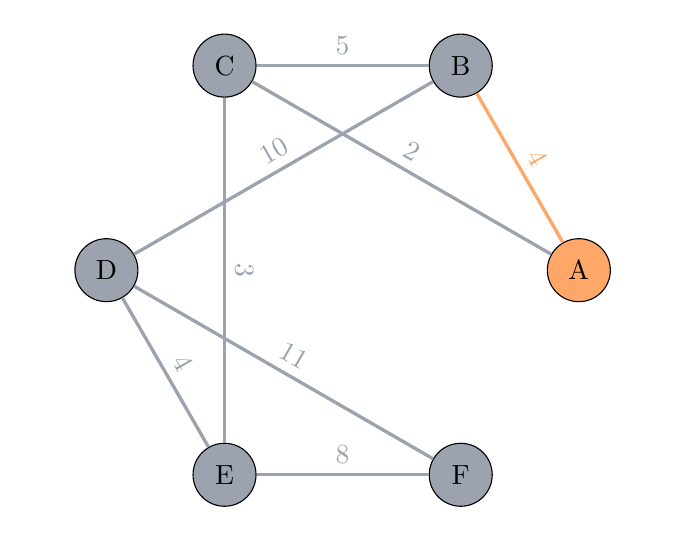
\begin{tikzpicture}
  \filldraw[fill=white!0, draw=none] (-4cm,0) rectangle (4cm, -3cm);
  \node[circle, draw, minimum size=8mm, fill=vizComparing] (A) at (0.0:3cm) {A};
  \node[circle, draw, minimum size=8mm, fill=vizDefault] (B) at (60.0:3cm) {B};
  \node[circle, draw, minimum size=8mm, fill=vizDefault] (C) at (120.0:3cm) {C};
  \node[circle, draw, minimum size=8mm, fill=vizDefault] (D) at (180.0:3cm) {D};
  \node[circle, draw, minimum size=8mm, fill=vizDefault] (E) at (240.0:3cm) {E};
  \node[circle, draw, minimum size=8mm, fill=vizDefault] (F) at (300.0:3cm) {F};
  \draw[vizComparing, line width=1.2pt] (A) -- node[midway, sloped, above] {4} (B);
  \draw[vizDefault, line width=1.2pt] (A) -- node[midway, sloped, above] {2} (C);
  \draw[vizDefault, line width=1.2pt] (B) -- node[midway, sloped, above] {5} (C);
  \draw[vizDefault, line width=1.2pt] (B) -- node[midway, sloped, above] {10} (D);
  \draw[vizDefault, line width=1.2pt] (C) -- node[midway, sloped, above] {3} (E);
  \draw[vizDefault, line width=1.2pt] (D) -- node[midway, sloped, above] {11} (F);
  \draw[vizDefault, line width=1.2pt] (E) -- node[midway, sloped, above] {4} (D);
  \draw[vizDefault, line width=1.2pt] (E) -- node[midway, sloped, above] {8} (F);
\end{tikzpicture}
\end{center}
\noindent\rule{\linewidth}{0.3pt}
\begin{center}
\begin{center}\textbf{Open Set}\\[1.75mm]\end{center}
\begin{tikzpicture}
  \filldraw[fill=white!0, draw=none] (0cm,0cm) rectangle (0cm, -1cm);
\end{tikzpicture}
\end{center}
\noindent\rule{\linewidth}{0.3pt}
\begin{center}
\begin{center}\textbf{Closed Set}\\[1.75mm]\end{center}

\begin{tikzpicture}
  \filldraw[fill=white!0, draw=none] (0cm,0cm) rectangle (0.8cm, -1cm);
  \filldraw[fill=vizDefault] (0cm,-0.8cm) rectangle (0.8cm,0cm);
  \node at (0.4cm,-0.4cm) {A};
\end{tikzpicture}
\end{center}
\noindent\rule{\linewidth}{0.3pt}
\begin{center}
\begin{center}\textbf{Node Costs}\\[1.75mm]\end{center}
\begin{tikzpicture}
  \filldraw[fill=white!0, draw=none] (0cm,0) rectangle (0.5cm,3.5cm);
  \node[above] at (0.25cm,0cm) {0};
  \node[below] at (0.25cm,0) {A};
  \filldraw[fill=white!0, draw=none] (0.7cm,0) rectangle (1.2cm,3.5cm);
  \node[above] at (0.95cm,0cm) {0};
  \node[below] at (0.95cm,0) {B};
  \filldraw[fill=white!0, draw=none] (1.4cm,0) rectangle (1.9cm,3.5cm);
  \node[above] at (1.65cm,0cm) {0};
  \node[below] at (1.65cm,0) {C};
  \filldraw[fill=white!0, draw=none] (2.0999999999999996cm,0) rectangle (2.5999999999999996cm,3.5cm);
  \node[above] at (2.3499999999999996cm,0cm) {0};
  \node[below] at (2.3499999999999996cm,0) {D};
  \filldraw[fill=white!0, draw=none] (2.8cm,0) rectangle (3.3cm,3.5cm);
  \node[above] at (3.05cm,0cm) {0};
  \node[below] at (3.05cm,0) {E};
  \filldraw[fill=white!0, draw=none] (3.5cm,0) rectangle (4cm,3.5cm);
  \node[above] at (3.75cm,0cm) {0};
  \node[below] at (3.75cm,0) {F};
\end{tikzpicture}
\end{center}
\newpage
% --- Frame 5 ---
\begin{center}\LARGE\textbf{Dijkstra}\\[6mm]\end{center}
\begin{center}
\begin{center}\textbf{Log}\\[1.75mm]\end{center}

\begin{tikzpicture}
  \filldraw[fill=white!0, draw=none] (0,0) rectangle (10cm, -0.25cm);
  \node[anchor=north, align=center, text=black] at (5cm,0) {\texttt{Neighbor B hasn't been seen yet — adding it to the open set.}};
\end{tikzpicture}
\end{center}
\noindent\rule{\linewidth}{0.3pt}
\begin{center}
\begin{center}\textbf{Graph}\\[2mm]\end{center}
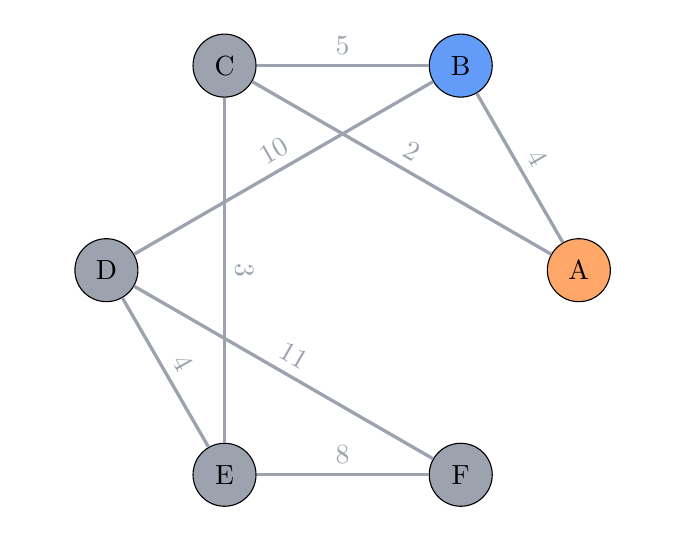
\begin{tikzpicture}
  \filldraw[fill=white!0, draw=none] (-4cm,0) rectangle (4cm, -3cm);
  \node[circle, draw, minimum size=8mm, fill=vizComparing] (A) at (0.0:3cm) {A};
  \node[circle, draw, minimum size=8mm, fill=vizActive] (B) at (60.0:3cm) {B};
  \node[circle, draw, minimum size=8mm, fill=vizDefault] (C) at (120.0:3cm) {C};
  \node[circle, draw, minimum size=8mm, fill=vizDefault] (D) at (180.0:3cm) {D};
  \node[circle, draw, minimum size=8mm, fill=vizDefault] (E) at (240.0:3cm) {E};
  \node[circle, draw, minimum size=8mm, fill=vizDefault] (F) at (300.0:3cm) {F};
  \draw[vizDefault, line width=1.2pt] (A) -- node[midway, sloped, above] {4} (B);
  \draw[vizDefault, line width=1.2pt] (A) -- node[midway, sloped, above] {2} (C);
  \draw[vizDefault, line width=1.2pt] (B) -- node[midway, sloped, above] {5} (C);
  \draw[vizDefault, line width=1.2pt] (B) -- node[midway, sloped, above] {10} (D);
  \draw[vizDefault, line width=1.2pt] (C) -- node[midway, sloped, above] {3} (E);
  \draw[vizDefault, line width=1.2pt] (D) -- node[midway, sloped, above] {11} (F);
  \draw[vizDefault, line width=1.2pt] (E) -- node[midway, sloped, above] {4} (D);
  \draw[vizDefault, line width=1.2pt] (E) -- node[midway, sloped, above] {8} (F);
\end{tikzpicture}
\end{center}
\noindent\rule{\linewidth}{0.3pt}
\begin{center}
\begin{center}\textbf{Open Set}\\[1.75mm]\end{center}
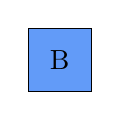
\begin{tikzpicture}
  \filldraw[fill=white!0, draw=none] (0cm,0cm) rectangle (0.8cm, -1cm);
  \filldraw[fill=vizActive] (0cm,-0.8cm) rectangle (0.8cm,0cm);
  \node at (0.4cm,-0.4cm) {B};
\end{tikzpicture}
\end{center}
\noindent\rule{\linewidth}{0.3pt}
\begin{center}
\begin{center}\textbf{Closed Set}\\[1.75mm]\end{center}

\begin{tikzpicture}
  \filldraw[fill=white!0, draw=none] (0cm,0cm) rectangle (0.8cm, -1cm);
  \filldraw[fill=vizDefault] (0cm,-0.8cm) rectangle (0.8cm,0cm);
  \node at (0.4cm,-0.4cm) {A};
\end{tikzpicture}
\end{center}
\noindent\rule{\linewidth}{0.3pt}
\begin{center}
\begin{center}\textbf{Node Costs}\\[1.75mm]\end{center}
\begin{tikzpicture}
  \filldraw[fill=white!0, draw=none] (0cm,0) rectangle (0.5cm,3.5cm);
  \node[above] at (0.25cm,0cm) {0};
  \node[below] at (0.25cm,0) {A};
  \filldraw[fill=white!0, draw=none] (0.7cm,0) rectangle (1.2cm,3.5cm);
  \node[above] at (0.95cm,0cm) {0};
  \node[below] at (0.95cm,0) {B};
  \filldraw[fill=white!0, draw=none] (1.4cm,0) rectangle (1.9cm,3.5cm);
  \node[above] at (1.65cm,0cm) {0};
  \node[below] at (1.65cm,0) {C};
  \filldraw[fill=white!0, draw=none] (2.0999999999999996cm,0) rectangle (2.5999999999999996cm,3.5cm);
  \node[above] at (2.3499999999999996cm,0cm) {0};
  \node[below] at (2.3499999999999996cm,0) {D};
  \filldraw[fill=white!0, draw=none] (2.8cm,0) rectangle (3.3cm,3.5cm);
  \node[above] at (3.05cm,0cm) {0};
  \node[below] at (3.05cm,0) {E};
  \filldraw[fill=white!0, draw=none] (3.5cm,0) rectangle (4cm,3.5cm);
  \node[above] at (3.75cm,0cm) {0};
  \node[below] at (3.75cm,0) {F};
\end{tikzpicture}
\end{center}
\newpage
% --- Frame 6 ---
\begin{center}\LARGE\textbf{Dijkstra}\\[6mm]\end{center}
\begin{center}
\begin{center}\textbf{Log}\\[1.75mm]\end{center}

\begin{tikzpicture}
  \filldraw[fill=white!0, draw=none] (0,0) rectangle (10cm, -0.25cm);
  \node[anchor=north, align=center, text=black] at (5cm,0) {\texttt{Found a cheaper path to B through A — updating its cost to 4.}};
\end{tikzpicture}
\end{center}
\noindent\rule{\linewidth}{0.3pt}
\begin{center}
\begin{center}\textbf{Graph}\\[2mm]\end{center}
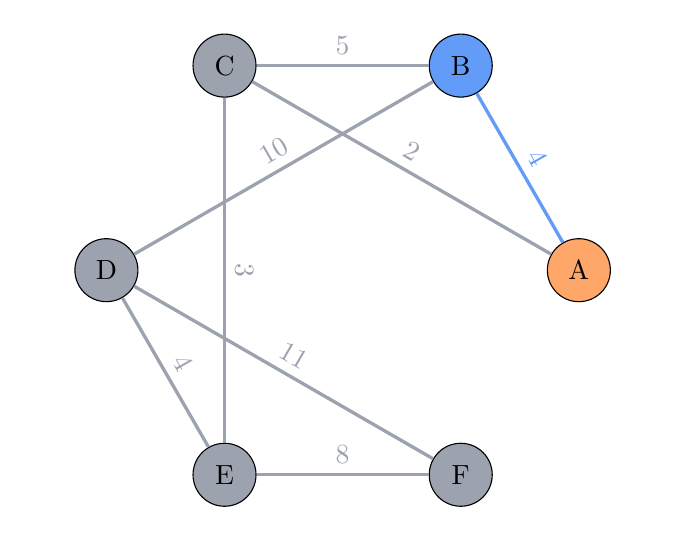
\begin{tikzpicture}
  \filldraw[fill=white!0, draw=none] (-4cm,0) rectangle (4cm, -3cm);
  \node[circle, draw, minimum size=8mm, fill=vizComparing] (A) at (0.0:3cm) {A};
  \node[circle, draw, minimum size=8mm, fill=vizActive] (B) at (60.0:3cm) {B};
  \node[circle, draw, minimum size=8mm, fill=vizDefault] (C) at (120.0:3cm) {C};
  \node[circle, draw, minimum size=8mm, fill=vizDefault] (D) at (180.0:3cm) {D};
  \node[circle, draw, minimum size=8mm, fill=vizDefault] (E) at (240.0:3cm) {E};
  \node[circle, draw, minimum size=8mm, fill=vizDefault] (F) at (300.0:3cm) {F};
  \draw[vizActive, line width=1.2pt] (A) -- node[midway, sloped, above] {4} (B);
  \draw[vizDefault, line width=1.2pt] (A) -- node[midway, sloped, above] {2} (C);
  \draw[vizDefault, line width=1.2pt] (B) -- node[midway, sloped, above] {5} (C);
  \draw[vizDefault, line width=1.2pt] (B) -- node[midway, sloped, above] {10} (D);
  \draw[vizDefault, line width=1.2pt] (C) -- node[midway, sloped, above] {3} (E);
  \draw[vizDefault, line width=1.2pt] (D) -- node[midway, sloped, above] {11} (F);
  \draw[vizDefault, line width=1.2pt] (E) -- node[midway, sloped, above] {4} (D);
  \draw[vizDefault, line width=1.2pt] (E) -- node[midway, sloped, above] {8} (F);
\end{tikzpicture}
\end{center}
\noindent\rule{\linewidth}{0.3pt}
\begin{center}
\begin{center}\textbf{Open Set}\\[1.75mm]\end{center}
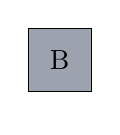
\begin{tikzpicture}
  \filldraw[fill=white!0, draw=none] (0cm,0cm) rectangle (0.8cm, -1cm);
  \filldraw[fill=vizDefault] (0cm,-0.8cm) rectangle (0.8cm,0cm);
  \node at (0.4cm,-0.4cm) {B};
\end{tikzpicture}
\end{center}
\noindent\rule{\linewidth}{0.3pt}
\begin{center}
\begin{center}\textbf{Closed Set}\\[1.75mm]\end{center}

\begin{tikzpicture}
  \filldraw[fill=white!0, draw=none] (0cm,0cm) rectangle (0.8cm, -1cm);
  \filldraw[fill=vizDefault] (0cm,-0.8cm) rectangle (0.8cm,0cm);
  \node at (0.4cm,-0.4cm) {A};
\end{tikzpicture}
\end{center}
\noindent\rule{\linewidth}{0.3pt}
\begin{center}
\begin{center}\textbf{Node Costs}\\[1.75mm]\end{center}
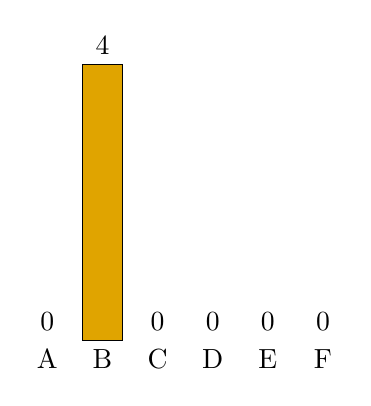
\begin{tikzpicture}
  \filldraw[fill=white!0, draw=none] (0cm,0) rectangle (0.5cm,3.5cm);
  \node[above] at (0.25cm,0cm) {0};
  \node[below] at (0.25cm,0) {A};
  \filldraw[fill=white!0, draw=none] (0.7cm,0) rectangle (1.2cm,3.5cm);
  \filldraw[fill=vizUpdated] (0.7cm,0cm) rectangle (1.2cm,3.5cm);
  \node[above] at (0.95cm,3.5cm) {4};
  \node[below] at (0.95cm,0) {B};
  \filldraw[fill=white!0, draw=none] (1.4cm,0) rectangle (1.9cm,3.5cm);
  \node[above] at (1.65cm,0cm) {0};
  \node[below] at (1.65cm,0) {C};
  \filldraw[fill=white!0, draw=none] (2.0999999999999996cm,0) rectangle (2.5999999999999996cm,3.5cm);
  \node[above] at (2.3499999999999996cm,0cm) {0};
  \node[below] at (2.3499999999999996cm,0) {D};
  \filldraw[fill=white!0, draw=none] (2.8cm,0) rectangle (3.3cm,3.5cm);
  \node[above] at (3.05cm,0cm) {0};
  \node[below] at (3.05cm,0) {E};
  \filldraw[fill=white!0, draw=none] (3.5cm,0) rectangle (4cm,3.5cm);
  \node[above] at (3.75cm,0cm) {0};
  \node[below] at (3.75cm,0) {F};
\end{tikzpicture}
\end{center}
\newpage
% --- Frame 7 ---
\begin{center}\LARGE\textbf{Dijkstra}\\[6mm]\end{center}
\begin{center}
\begin{center}\textbf{Log}\\[1.75mm]\end{center}

\begin{tikzpicture}
  \filldraw[fill=white!0, draw=none] (0,0) rectangle (10cm, -0.25cm);
  \node[anchor=north, align=center, text=black] at (5cm,0) {\texttt{Looking at neighbor C — is going through A cheaper than what we already know?}};
\end{tikzpicture}
\end{center}
\noindent\rule{\linewidth}{0.3pt}
\begin{center}
\begin{center}\textbf{Graph}\\[2mm]\end{center}
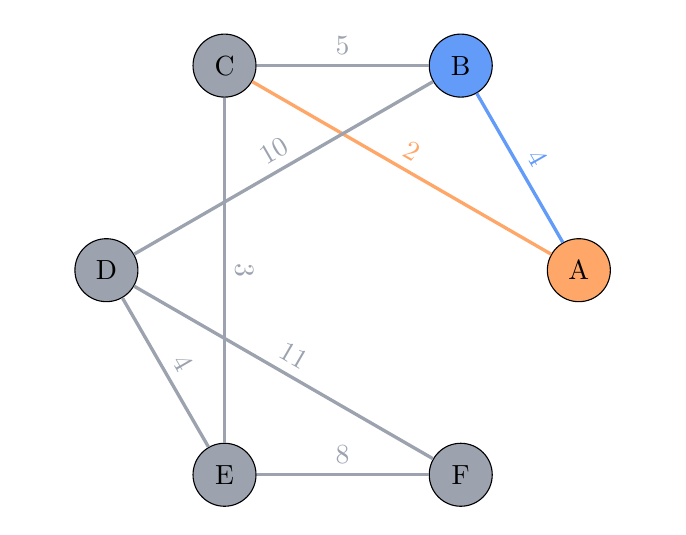
\begin{tikzpicture}
  \filldraw[fill=white!0, draw=none] (-4cm,0) rectangle (4cm, -3cm);
  \node[circle, draw, minimum size=8mm, fill=vizComparing] (A) at (0.0:3cm) {A};
  \node[circle, draw, minimum size=8mm, fill=vizActive] (B) at (60.0:3cm) {B};
  \node[circle, draw, minimum size=8mm, fill=vizDefault] (C) at (120.0:3cm) {C};
  \node[circle, draw, minimum size=8mm, fill=vizDefault] (D) at (180.0:3cm) {D};
  \node[circle, draw, minimum size=8mm, fill=vizDefault] (E) at (240.0:3cm) {E};
  \node[circle, draw, minimum size=8mm, fill=vizDefault] (F) at (300.0:3cm) {F};
  \draw[vizActive, line width=1.2pt] (A) -- node[midway, sloped, above] {4} (B);
  \draw[vizComparing, line width=1.2pt] (A) -- node[midway, sloped, above] {2} (C);
  \draw[vizDefault, line width=1.2pt] (B) -- node[midway, sloped, above] {5} (C);
  \draw[vizDefault, line width=1.2pt] (B) -- node[midway, sloped, above] {10} (D);
  \draw[vizDefault, line width=1.2pt] (C) -- node[midway, sloped, above] {3} (E);
  \draw[vizDefault, line width=1.2pt] (D) -- node[midway, sloped, above] {11} (F);
  \draw[vizDefault, line width=1.2pt] (E) -- node[midway, sloped, above] {4} (D);
  \draw[vizDefault, line width=1.2pt] (E) -- node[midway, sloped, above] {8} (F);
\end{tikzpicture}
\end{center}
\noindent\rule{\linewidth}{0.3pt}
\begin{center}
\begin{center}\textbf{Open Set}\\[1.75mm]\end{center}
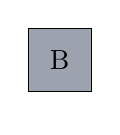
\begin{tikzpicture}
  \filldraw[fill=white!0, draw=none] (0cm,0cm) rectangle (0.8cm, -1cm);
  \filldraw[fill=vizDefault] (0cm,-0.8cm) rectangle (0.8cm,0cm);
  \node at (0.4cm,-0.4cm) {B};
\end{tikzpicture}
\end{center}
\noindent\rule{\linewidth}{0.3pt}
\begin{center}
\begin{center}\textbf{Closed Set}\\[1.75mm]\end{center}

\begin{tikzpicture}
  \filldraw[fill=white!0, draw=none] (0cm,0cm) rectangle (0.8cm, -1cm);
  \filldraw[fill=vizDefault] (0cm,-0.8cm) rectangle (0.8cm,0cm);
  \node at (0.4cm,-0.4cm) {A};
\end{tikzpicture}
\end{center}
\noindent\rule{\linewidth}{0.3pt}
\begin{center}
\begin{center}\textbf{Node Costs}\\[1.75mm]\end{center}
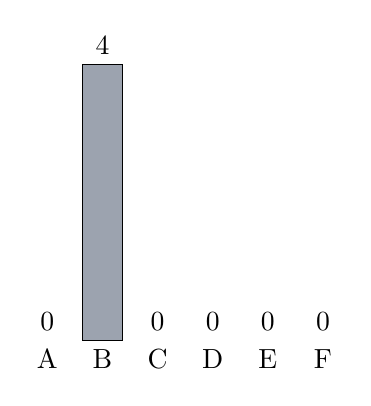
\begin{tikzpicture}
  \filldraw[fill=white!0, draw=none] (0cm,0) rectangle (0.5cm,3.5cm);
  \node[above] at (0.25cm,0cm) {0};
  \node[below] at (0.25cm,0) {A};
  \filldraw[fill=white!0, draw=none] (0.7cm,0) rectangle (1.2cm,3.5cm);
  \filldraw[fill=vizDefault] (0.7cm,0) rectangle (1.2cm,3.5cm);
  \node[above] at (0.95cm,3.5cm) {4};
  \node[below] at (0.95cm,0) {B};
  \filldraw[fill=white!0, draw=none] (1.4cm,0) rectangle (1.9cm,3.5cm);
  \node[above] at (1.65cm,0cm) {0};
  \node[below] at (1.65cm,0) {C};
  \filldraw[fill=white!0, draw=none] (2.0999999999999996cm,0) rectangle (2.5999999999999996cm,3.5cm);
  \node[above] at (2.3499999999999996cm,0cm) {0};
  \node[below] at (2.3499999999999996cm,0) {D};
  \filldraw[fill=white!0, draw=none] (2.8cm,0) rectangle (3.3cm,3.5cm);
  \node[above] at (3.05cm,0cm) {0};
  \node[below] at (3.05cm,0) {E};
  \filldraw[fill=white!0, draw=none] (3.5cm,0) rectangle (4cm,3.5cm);
  \node[above] at (3.75cm,0cm) {0};
  \node[below] at (3.75cm,0) {F};
\end{tikzpicture}
\end{center}
\newpage
% --- Frame 8 ---
\begin{center}\LARGE\textbf{Dijkstra}\\[6mm]\end{center}
\begin{center}
\begin{center}\textbf{Log}\\[1.75mm]\end{center}

\begin{tikzpicture}
  \filldraw[fill=white!0, draw=none] (0,0) rectangle (10cm, -0.25cm);
  \node[anchor=north, align=center, text=black] at (5cm,0) {\texttt{Neighbor C hasn't been seen yet — adding it to the open set.}};
\end{tikzpicture}
\end{center}
\noindent\rule{\linewidth}{0.3pt}
\begin{center}
\begin{center}\textbf{Graph}\\[2mm]\end{center}
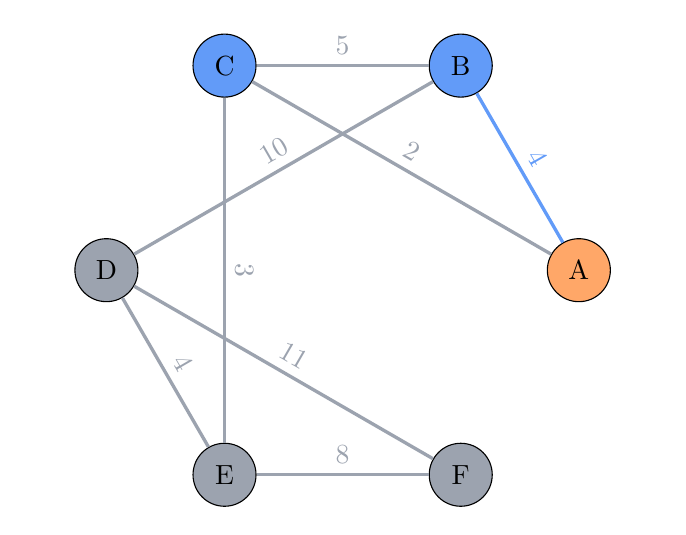
\begin{tikzpicture}
  \filldraw[fill=white!0, draw=none] (-4cm,0) rectangle (4cm, -3cm);
  \node[circle, draw, minimum size=8mm, fill=vizComparing] (A) at (0.0:3cm) {A};
  \node[circle, draw, minimum size=8mm, fill=vizActive] (B) at (60.0:3cm) {B};
  \node[circle, draw, minimum size=8mm, fill=vizActive] (C) at (120.0:3cm) {C};
  \node[circle, draw, minimum size=8mm, fill=vizDefault] (D) at (180.0:3cm) {D};
  \node[circle, draw, minimum size=8mm, fill=vizDefault] (E) at (240.0:3cm) {E};
  \node[circle, draw, minimum size=8mm, fill=vizDefault] (F) at (300.0:3cm) {F};
  \draw[vizActive, line width=1.2pt] (A) -- node[midway, sloped, above] {4} (B);
  \draw[vizDefault, line width=1.2pt] (A) -- node[midway, sloped, above] {2} (C);
  \draw[vizDefault, line width=1.2pt] (B) -- node[midway, sloped, above] {5} (C);
  \draw[vizDefault, line width=1.2pt] (B) -- node[midway, sloped, above] {10} (D);
  \draw[vizDefault, line width=1.2pt] (C) -- node[midway, sloped, above] {3} (E);
  \draw[vizDefault, line width=1.2pt] (D) -- node[midway, sloped, above] {11} (F);
  \draw[vizDefault, line width=1.2pt] (E) -- node[midway, sloped, above] {4} (D);
  \draw[vizDefault, line width=1.2pt] (E) -- node[midway, sloped, above] {8} (F);
\end{tikzpicture}
\end{center}
\noindent\rule{\linewidth}{0.3pt}
\begin{center}
\begin{center}\textbf{Open Set}\\[1.75mm]\end{center}
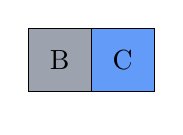
\begin{tikzpicture}
  \filldraw[fill=white!0, draw=none] (0cm,0cm) rectangle (1.6cm, -1cm);
  \filldraw[fill=vizDefault] (0cm,-0.8cm) rectangle (0.8cm,0cm);
  \node at (0.4cm,-0.4cm) {B};
  \filldraw[fill=vizActive] (0.8cm,-0.8cm) rectangle (1.6cm,0cm);
  \node at (1.2000000000000002cm,-0.4cm) {C};
\end{tikzpicture}
\end{center}
\noindent\rule{\linewidth}{0.3pt}
\begin{center}
\begin{center}\textbf{Closed Set}\\[1.75mm]\end{center}

\begin{tikzpicture}
  \filldraw[fill=white!0, draw=none] (0cm,0cm) rectangle (0.8cm, -1cm);
  \filldraw[fill=vizDefault] (0cm,-0.8cm) rectangle (0.8cm,0cm);
  \node at (0.4cm,-0.4cm) {A};
\end{tikzpicture}
\end{center}
\noindent\rule{\linewidth}{0.3pt}
\begin{center}
\begin{center}\textbf{Node Costs}\\[1.75mm]\end{center}
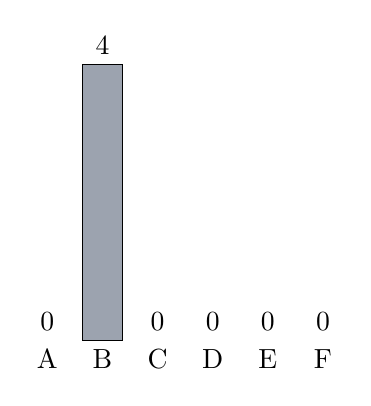
\begin{tikzpicture}
  \filldraw[fill=white!0, draw=none] (0cm,0) rectangle (0.5cm,3.5cm);
  \node[above] at (0.25cm,0cm) {0};
  \node[below] at (0.25cm,0) {A};
  \filldraw[fill=white!0, draw=none] (0.7cm,0) rectangle (1.2cm,3.5cm);
  \filldraw[fill=vizDefault] (0.7cm,0) rectangle (1.2cm,3.5cm);
  \node[above] at (0.95cm,3.5cm) {4};
  \node[below] at (0.95cm,0) {B};
  \filldraw[fill=white!0, draw=none] (1.4cm,0) rectangle (1.9cm,3.5cm);
  \node[above] at (1.65cm,0cm) {0};
  \node[below] at (1.65cm,0) {C};
  \filldraw[fill=white!0, draw=none] (2.0999999999999996cm,0) rectangle (2.5999999999999996cm,3.5cm);
  \node[above] at (2.3499999999999996cm,0cm) {0};
  \node[below] at (2.3499999999999996cm,0) {D};
  \filldraw[fill=white!0, draw=none] (2.8cm,0) rectangle (3.3cm,3.5cm);
  \node[above] at (3.05cm,0cm) {0};
  \node[below] at (3.05cm,0) {E};
  \filldraw[fill=white!0, draw=none] (3.5cm,0) rectangle (4cm,3.5cm);
  \node[above] at (3.75cm,0cm) {0};
  \node[below] at (3.75cm,0) {F};
\end{tikzpicture}
\end{center}
\newpage
% --- Frame 9 ---
\begin{center}\LARGE\textbf{Dijkstra}\\[6mm]\end{center}
\begin{center}
\begin{center}\textbf{Log}\\[1.75mm]\end{center}

\begin{tikzpicture}
  \filldraw[fill=white!0, draw=none] (0,0) rectangle (10cm, -0.25cm);
  \node[anchor=north, align=center, text=black] at (5cm,0) {\texttt{Found a cheaper path to C through A — updating its cost to 2.}};
\end{tikzpicture}
\end{center}
\noindent\rule{\linewidth}{0.3pt}
\begin{center}
\begin{center}\textbf{Graph}\\[2mm]\end{center}
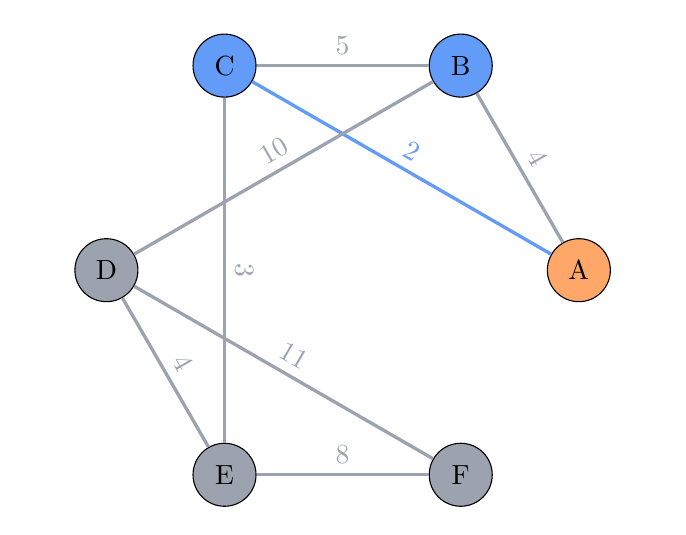
\begin{tikzpicture}
  \filldraw[fill=white!0, draw=none] (-4cm,0) rectangle (4cm, -3cm);
  \node[circle, draw, minimum size=8mm, fill=vizComparing] (A) at (0.0:3cm) {A};
  \node[circle, draw, minimum size=8mm, fill=vizActive] (B) at (60.0:3cm) {B};
  \node[circle, draw, minimum size=8mm, fill=vizActive] (C) at (120.0:3cm) {C};
  \node[circle, draw, minimum size=8mm, fill=vizDefault] (D) at (180.0:3cm) {D};
  \node[circle, draw, minimum size=8mm, fill=vizDefault] (E) at (240.0:3cm) {E};
  \node[circle, draw, minimum size=8mm, fill=vizDefault] (F) at (300.0:3cm) {F};
  \draw[vizDefault, line width=1.2pt] (A) -- node[midway, sloped, above] {4} (B);
  \draw[vizActive, line width=1.2pt] (A) -- node[midway, sloped, above] {2} (C);
  \draw[vizDefault, line width=1.2pt] (B) -- node[midway, sloped, above] {5} (C);
  \draw[vizDefault, line width=1.2pt] (B) -- node[midway, sloped, above] {10} (D);
  \draw[vizDefault, line width=1.2pt] (C) -- node[midway, sloped, above] {3} (E);
  \draw[vizDefault, line width=1.2pt] (D) -- node[midway, sloped, above] {11} (F);
  \draw[vizDefault, line width=1.2pt] (E) -- node[midway, sloped, above] {4} (D);
  \draw[vizDefault, line width=1.2pt] (E) -- node[midway, sloped, above] {8} (F);
\end{tikzpicture}
\end{center}
\noindent\rule{\linewidth}{0.3pt}
\begin{center}
\begin{center}\textbf{Open Set}\\[1.75mm]\end{center}
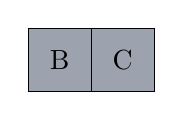
\begin{tikzpicture}
  \filldraw[fill=white!0, draw=none] (0cm,0cm) rectangle (1.6cm, -1cm);
  \filldraw[fill=vizDefault] (0cm,-0.8cm) rectangle (0.8cm,0cm);
  \node at (0.4cm,-0.4cm) {B};
  \filldraw[fill=vizDefault] (0.8cm,-0.8cm) rectangle (1.6cm,0cm);
  \node at (1.2000000000000002cm,-0.4cm) {C};
\end{tikzpicture}
\end{center}
\noindent\rule{\linewidth}{0.3pt}
\begin{center}
\begin{center}\textbf{Closed Set}\\[1.75mm]\end{center}

\begin{tikzpicture}
  \filldraw[fill=white!0, draw=none] (0cm,0cm) rectangle (0.8cm, -1cm);
  \filldraw[fill=vizDefault] (0cm,-0.8cm) rectangle (0.8cm,0cm);
  \node at (0.4cm,-0.4cm) {A};
\end{tikzpicture}
\end{center}
\noindent\rule{\linewidth}{0.3pt}
\begin{center}
\begin{center}\textbf{Node Costs}\\[1.75mm]\end{center}
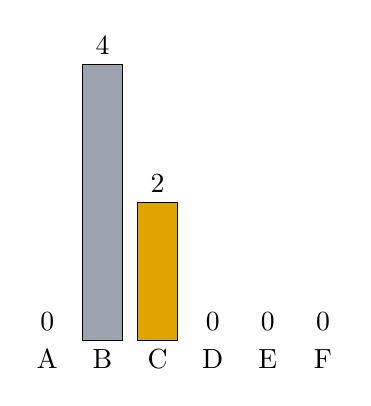
\begin{tikzpicture}
  \filldraw[fill=white!0, draw=none] (0cm,0) rectangle (0.5cm,3.5cm);
  \node[above] at (0.25cm,0cm) {0};
  \node[below] at (0.25cm,0) {A};
  \filldraw[fill=white!0, draw=none] (0.7cm,0) rectangle (1.2cm,3.5cm);
  \filldraw[fill=vizDefault] (0.7cm,0) rectangle (1.2cm,3.5cm);
  \node[above] at (0.95cm,3.5cm) {4};
  \node[below] at (0.95cm,0) {B};
  \filldraw[fill=white!0, draw=none] (1.4cm,0) rectangle (1.9cm,3.5cm);
  \filldraw[fill=vizUpdated] (1.4cm,0cm) rectangle (1.9cm,1.75cm);
  \node[above] at (1.65cm,1.75cm) {2};
  \node[below] at (1.65cm,0) {C};
  \filldraw[fill=white!0, draw=none] (2.0999999999999996cm,0) rectangle (2.5999999999999996cm,3.5cm);
  \node[above] at (2.3499999999999996cm,0cm) {0};
  \node[below] at (2.3499999999999996cm,0) {D};
  \filldraw[fill=white!0, draw=none] (2.8cm,0) rectangle (3.3cm,3.5cm);
  \node[above] at (3.05cm,0cm) {0};
  \node[below] at (3.05cm,0) {E};
  \filldraw[fill=white!0, draw=none] (3.5cm,0) rectangle (4cm,3.5cm);
  \node[above] at (3.75cm,0cm) {0};
  \node[below] at (3.75cm,0) {F};
\end{tikzpicture}
\end{center}
\newpage
% --- Frame 10 ---
\begin{center}\LARGE\textbf{Dijkstra}\\[6mm]\end{center}
\begin{center}
\begin{center}\textbf{Log}\\[1.75mm]\end{center}
\begin{tikzpicture}
  \filldraw[fill=white!0, draw=none] (0,0) rectangle (10cm, -0.25cm);
  \node[anchor=north, align=center, text=black] at (5cm,0) {\texttt{Sorting the open set so the lowest-cost node comes first.}};
\end{tikzpicture}
\end{center}
\noindent\rule{\linewidth}{0.3pt}
\begin{center}
\begin{center}\textbf{Graph}\\[2mm]\end{center}
\begin{tikzpicture}
  \filldraw[fill=white!0, draw=none] (-4cm,0) rectangle (4cm, -3cm);
  \node[circle, draw, minimum size=8mm, fill=vizSorted] (A) at (0.0:3cm) {A};
  \node[circle, draw, minimum size=8mm, fill=vizActive] (B) at (60.0:3cm) {B};
  \node[circle, draw, minimum size=8mm, fill=vizActive] (C) at (120.0:3cm) {C};
  \node[circle, draw, minimum size=8mm, fill=vizDefault] (D) at (180.0:3cm) {D};
  \node[circle, draw, minimum size=8mm, fill=vizDefault] (E) at (240.0:3cm) {E};
  \node[circle, draw, minimum size=8mm, fill=vizDefault] (F) at (300.0:3cm) {F};
  \draw[vizDefault, line width=1.2pt] (A) -- node[midway, sloped, above] {4} (B);
  \draw[vizActive, line width=1.2pt] (A) -- node[midway, sloped, above] {2} (C);
  \draw[vizDefault, line width=1.2pt] (B) -- node[midway, sloped, above] {5} (C);
  \draw[vizDefault, line width=1.2pt] (B) -- node[midway, sloped, above] {10} (D);
  \draw[vizDefault, line width=1.2pt] (C) -- node[midway, sloped, above] {3} (E);
  \draw[vizDefault, line width=1.2pt] (D) -- node[midway, sloped, above] {11} (F);
  \draw[vizDefault, line width=1.2pt] (E) -- node[midway, sloped, above] {4} (D);
  \draw[vizDefault, line width=1.2pt] (E) -- node[midway, sloped, above] {8} (F);
\end{tikzpicture}
\end{center}
\noindent\rule{\linewidth}{0.3pt}
\begin{center}
\begin{center}\textbf{Open Set}\\[1.75mm]\end{center}
\begin{tikzpicture}
  \filldraw[fill=white!0, draw=none] (0cm,0cm) rectangle (1.6cm, -1cm);
  \filldraw[fill=vizComparing] (0cm,-0.8cm) rectangle (0.8cm,0cm);
  \node at (0.4cm,-0.4cm) {C};
  \filldraw[fill=vizComparing] (0.8cm,-0.8cm) rectangle (1.6cm,0cm);
  \node at (1.2000000000000002cm,-0.4cm) {B};
\end{tikzpicture}
\end{center}
\noindent\rule{\linewidth}{0.3pt}
\begin{center}
\begin{center}\textbf{Closed Set}\\[1.75mm]\end{center}
\begin{tikzpicture}
  \filldraw[fill=white!0, draw=none] (0cm,0cm) rectangle (0.8cm, -1cm);
  \filldraw[fill=vizDefault] (0cm,-0.8cm) rectangle (0.8cm,0cm);
  \node at (0.4cm,-0.4cm) {A};
\end{tikzpicture}
\end{center}
\noindent\rule{\linewidth}{0.3pt}
\begin{center}
\begin{center}\textbf{Node Costs}\\[1.75mm]\end{center}
\begin{tikzpicture}
  \filldraw[fill=white!0, draw=none] (0cm,0) rectangle (0.5cm,3.5cm);
  \node[above] at (0.25cm,0cm) {0};
  \node[below] at (0.25cm,0) {A};
  \filldraw[fill=white!0, draw=none] (0.7cm,0) rectangle (1.2cm,3.5cm);
  \filldraw[fill=vizDefault] (0.7cm,0) rectangle (1.2cm,3.5cm);
  \node[above] at (0.95cm,3.5cm) {4};
  \node[below] at (0.95cm,0) {B};
  \filldraw[fill=white!0, draw=none] (1.4cm,0) rectangle (1.9cm,3.5cm);
  \filldraw[fill=vizDefault] (1.4cm,0) rectangle (1.9cm,1.75cm);
  \node[above] at (1.65cm,1.75cm) {2};
  \node[below] at (1.65cm,0) {C};
  \filldraw[fill=white!0, draw=none] (2.0999999999999996cm,0) rectangle (2.5999999999999996cm,3.5cm);
  \node[above] at (2.3499999999999996cm,0cm) {0};
  \node[below] at (2.3499999999999996cm,0) {D};
  \filldraw[fill=white!0, draw=none] (2.8cm,0) rectangle (3.3cm,3.5cm);
  \node[above] at (3.05cm,0cm) {0};
  \node[below] at (3.05cm,0) {E};
  \filldraw[fill=white!0, draw=none] (3.5cm,0) rectangle (4cm,3.5cm);
  \node[above] at (3.75cm,0cm) {0};
  \node[below] at (3.75cm,0) {F};
\end{tikzpicture}
\end{center}
\newpage
% --- Frame 11 ---
\begin{center}\LARGE\textbf{Dijkstra}\\[6mm]\end{center}
\begin{center}
\begin{center}\textbf{Log}\\[1.75mm]\end{center}
\begin{tikzpicture}
  \filldraw[fill=white!0, draw=none] (0,0) rectangle (10cm, -0.25cm);
  \node[anchor=north, align=center, text=black] at (5cm,0) {\texttt{Grabbing the lowest-cost node from the open set.}};
\end{tikzpicture}
\end{center}
\noindent\rule{\linewidth}{0.3pt}
\begin{center}
\begin{center}\textbf{Graph}\\[2mm]\end{center}
\begin{tikzpicture}
  \filldraw[fill=white!0, draw=none] (-4cm,0) rectangle (4cm, -3cm);
  \node[circle, draw, minimum size=8mm, fill=vizSorted] (A) at (0.0:3cm) {A};
  \node[circle, draw, minimum size=8mm, fill=vizActive] (B) at (60.0:3cm) {B};
  \node[circle, draw, minimum size=8mm, fill=vizActive] (C) at (120.0:3cm) {C};
  \node[circle, draw, minimum size=8mm, fill=vizDefault] (D) at (180.0:3cm) {D};
  \node[circle, draw, minimum size=8mm, fill=vizDefault] (E) at (240.0:3cm) {E};
  \node[circle, draw, minimum size=8mm, fill=vizDefault] (F) at (300.0:3cm) {F};
  \draw[vizDefault, line width=1.2pt] (A) -- node[midway, sloped, above] {4} (B);
  \draw[vizActive, line width=1.2pt] (A) -- node[midway, sloped, above] {2} (C);
  \draw[vizDefault, line width=1.2pt] (B) -- node[midway, sloped, above] {5} (C);
  \draw[vizDefault, line width=1.2pt] (B) -- node[midway, sloped, above] {10} (D);
  \draw[vizDefault, line width=1.2pt] (C) -- node[midway, sloped, above] {3} (E);
  \draw[vizDefault, line width=1.2pt] (D) -- node[midway, sloped, above] {11} (F);
  \draw[vizDefault, line width=1.2pt] (E) -- node[midway, sloped, above] {4} (D);
  \draw[vizDefault, line width=1.2pt] (E) -- node[midway, sloped, above] {8} (F);
\end{tikzpicture}
\end{center}
\noindent\rule{\linewidth}{0.3pt}
\begin{center}
\begin{center}\textbf{Open Set}\\[1.75mm]\end{center}
\begin{tikzpicture}
  \filldraw[fill=white!0, draw=none] (0cm,0cm) rectangle (1.6cm, -1cm);
  \filldraw[fill=vizSwapping] (0cm,-0.8cm) rectangle (0.8cm,0cm);
  \node at (0.4cm,-0.4cm) {C};
  \filldraw[fill=vizDefault] (0.8cm,-0.8cm) rectangle (1.6cm,0cm);
  \node at (1.2000000000000002cm,-0.4cm) {B};
\end{tikzpicture}
\end{center}
\noindent\rule{\linewidth}{0.3pt}
\begin{center}
\begin{center}\textbf{Closed Set}\\[1.75mm]\end{center}
\begin{tikzpicture}
  \filldraw[fill=white!0, draw=none] (0cm,0cm) rectangle (0.8cm, -1cm);
  \filldraw[fill=vizDefault] (0cm,-0.8cm) rectangle (0.8cm,0cm);
  \node at (0.4cm,-0.4cm) {A};
\end{tikzpicture}
\end{center}
\noindent\rule{\linewidth}{0.3pt}
\begin{center}
\begin{center}\textbf{Node Costs}\\[1.75mm]\end{center}
\begin{tikzpicture}
  \filldraw[fill=white!0, draw=none] (0cm,0) rectangle (0.5cm,3.5cm);
  \node[above] at (0.25cm,0cm) {0};
  \node[below] at (0.25cm,0) {A};
  \filldraw[fill=white!0, draw=none] (0.7cm,0) rectangle (1.2cm,3.5cm);
  \filldraw[fill=vizDefault] (0.7cm,0) rectangle (1.2cm,3.5cm);
  \node[above] at (0.95cm,3.5cm) {4};
  \node[below] at (0.95cm,0) {B};
  \filldraw[fill=white!0, draw=none] (1.4cm,0) rectangle (1.9cm,3.5cm);
  \filldraw[fill=vizDefault] (1.4cm,0) rectangle (1.9cm,1.75cm);
  \node[above] at (1.65cm,1.75cm) {2};
  \node[below] at (1.65cm,0) {C};
  \filldraw[fill=white!0, draw=none] (2.0999999999999996cm,0) rectangle (2.5999999999999996cm,3.5cm);
  \node[above] at (2.3499999999999996cm,0cm) {0};
  \node[below] at (2.3499999999999996cm,0) {D};
  \filldraw[fill=white!0, draw=none] (2.8cm,0) rectangle (3.3cm,3.5cm);
  \node[above] at (3.05cm,0cm) {0};
  \node[below] at (3.05cm,0) {E};
  \filldraw[fill=white!0, draw=none] (3.5cm,0) rectangle (4cm,3.5cm);
  \node[above] at (3.75cm,0cm) {0};
  \node[below] at (3.75cm,0) {F};
\end{tikzpicture}
\end{center}
\newpage
% --- Frame 12 ---
\begin{center}\LARGE\textbf{Dijkstra}\\[6mm]\end{center}
\begin{center}
\begin{center}\textbf{Log}\\[1.75mm]\end{center}
\begin{tikzpicture}
  \filldraw[fill=white!0, draw=none] (0,0) rectangle (10cm, -0.25cm);
  \node[anchor=north, align=center, text=black] at (5cm,0) {\texttt{Visiting node C and moving it to the closed set.}};
\end{tikzpicture}
\end{center}
\noindent\rule{\linewidth}{0.3pt}
\begin{center}
\begin{center}\textbf{Graph}\\[2mm]\end{center}
\begin{tikzpicture}
  \filldraw[fill=white!0, draw=none] (-4cm,0) rectangle (4cm, -3cm);
  \node[circle, draw, minimum size=8mm, fill=vizSorted] (A) at (0.0:3cm) {A};
  \node[circle, draw, minimum size=8mm, fill=vizActive] (B) at (60.0:3cm) {B};
  \node[circle, draw, minimum size=8mm, fill=vizComparing] (C) at (120.0:3cm) {C};
  \node[circle, draw, minimum size=8mm, fill=vizDefault] (D) at (180.0:3cm) {D};
  \node[circle, draw, minimum size=8mm, fill=vizDefault] (E) at (240.0:3cm) {E};
  \node[circle, draw, minimum size=8mm, fill=vizDefault] (F) at (300.0:3cm) {F};
  \draw[vizDefault, line width=1.2pt] (A) -- node[midway, sloped, above] {4} (B);
  \draw[vizActive, line width=1.2pt] (A) -- node[midway, sloped, above] {2} (C);
  \draw[vizDefault, line width=1.2pt] (B) -- node[midway, sloped, above] {5} (C);
  \draw[vizDefault, line width=1.2pt] (B) -- node[midway, sloped, above] {10} (D);
  \draw[vizDefault, line width=1.2pt] (C) -- node[midway, sloped, above] {3} (E);
  \draw[vizDefault, line width=1.2pt] (D) -- node[midway, sloped, above] {11} (F);
  \draw[vizDefault, line width=1.2pt] (E) -- node[midway, sloped, above] {4} (D);
  \draw[vizDefault, line width=1.2pt] (E) -- node[midway, sloped, above] {8} (F);
\end{tikzpicture}
\end{center}
\noindent\rule{\linewidth}{0.3pt}
\begin{center}
\begin{center}\textbf{Open Set}\\[1.75mm]\end{center}
\begin{tikzpicture}
  \filldraw[fill=white!0, draw=none] (0cm,0cm) rectangle (0.8cm, -1cm);
  \filldraw[fill=vizDefault] (0cm,-0.8cm) rectangle (0.8cm,0cm);
  \node at (0.4cm,-0.4cm) {B};
\end{tikzpicture}
\end{center}
\noindent\rule{\linewidth}{0.3pt}
\begin{center}
\begin{center}\textbf{Closed Set}\\[1.75mm]\end{center}
\begin{tikzpicture}
  \filldraw[fill=white!0, draw=none] (0cm,0cm) rectangle (1.6cm, -1cm);
  \filldraw[fill=vizDefault] (0cm,-0.8cm) rectangle (0.8cm,0cm);
  \node at (0.4cm,-0.4cm) {A};
  \filldraw[fill=vizActive] (0.8cm,-0.8cm) rectangle (1.6cm,0cm);
  \node at (1.2000000000000002cm,-0.4cm) {C};
\end{tikzpicture}
\end{center}
\noindent\rule{\linewidth}{0.3pt}
\begin{center}
\begin{center}\textbf{Node Costs}\\[1.75mm]\end{center}
\begin{tikzpicture}
  \filldraw[fill=white!0, draw=none] (0cm,0) rectangle (0.5cm,3.5cm);
  \node[above] at (0.25cm,0cm) {0};
  \node[below] at (0.25cm,0) {A};
  \filldraw[fill=white!0, draw=none] (0.7cm,0) rectangle (1.2cm,3.5cm);
  \filldraw[fill=vizDefault] (0.7cm,0) rectangle (1.2cm,3.5cm);
  \node[above] at (0.95cm,3.5cm) {4};
  \node[below] at (0.95cm,0) {B};
  \filldraw[fill=white!0, draw=none] (1.4cm,0) rectangle (1.9cm,3.5cm);
  \filldraw[fill=vizDefault] (1.4cm,0) rectangle (1.9cm,1.75cm);
  \node[above] at (1.65cm,1.75cm) {2};
  \node[below] at (1.65cm,0) {C};
  \filldraw[fill=white!0, draw=none] (2.0999999999999996cm,0) rectangle (2.5999999999999996cm,3.5cm);
  \node[above] at (2.3499999999999996cm,0cm) {0};
  \node[below] at (2.3499999999999996cm,0) {D};
  \filldraw[fill=white!0, draw=none] (2.8cm,0) rectangle (3.3cm,3.5cm);
  \node[above] at (3.05cm,0cm) {0};
  \node[below] at (3.05cm,0) {E};
  \filldraw[fill=white!0, draw=none] (3.5cm,0) rectangle (4cm,3.5cm);
  \node[above] at (3.75cm,0cm) {0};
  \node[below] at (3.75cm,0) {F};
\end{tikzpicture}
\end{center}
\newpage
% --- Frame 13 ---
\begin{center}\LARGE\textbf{Dijkstra}\\[6mm]\end{center}
\begin{center}
\begin{center}\textbf{Log}\\[1.75mm]\end{center}
\begin{tikzpicture}
  \filldraw[fill=white!0, draw=none] (0,0) rectangle (10cm, -0.25cm);
  \node[anchor=north, align=center, text=black] at (5cm,0) {\texttt{Looking at neighbor E — is going through C cheaper than what we already know?}};
\end{tikzpicture}
\end{center}
\noindent\rule{\linewidth}{0.3pt}
\begin{center}
\begin{center}\textbf{Graph}\\[2mm]\end{center}
\begin{tikzpicture}
  \filldraw[fill=white!0, draw=none] (-4cm,0) rectangle (4cm, -3cm);
  \node[circle, draw, minimum size=8mm, fill=vizSorted] (A) at (0.0:3cm) {A};
  \node[circle, draw, minimum size=8mm, fill=vizActive] (B) at (60.0:3cm) {B};
  \node[circle, draw, minimum size=8mm, fill=vizComparing] (C) at (120.0:3cm) {C};
  \node[circle, draw, minimum size=8mm, fill=vizDefault] (D) at (180.0:3cm) {D};
  \node[circle, draw, minimum size=8mm, fill=vizDefault] (E) at (240.0:3cm) {E};
  \node[circle, draw, minimum size=8mm, fill=vizDefault] (F) at (300.0:3cm) {F};
  \draw[vizDefault, line width=1.2pt] (A) -- node[midway, sloped, above] {4} (B);
  \draw[vizActive, line width=1.2pt] (A) -- node[midway, sloped, above] {2} (C);
  \draw[vizDefault, line width=1.2pt] (B) -- node[midway, sloped, above] {5} (C);
  \draw[vizDefault, line width=1.2pt] (B) -- node[midway, sloped, above] {10} (D);
  \draw[vizComparing, line width=1.2pt] (C) -- node[midway, sloped, above] {3} (E);
  \draw[vizDefault, line width=1.2pt] (D) -- node[midway, sloped, above] {11} (F);
  \draw[vizDefault, line width=1.2pt] (E) -- node[midway, sloped, above] {4} (D);
  \draw[vizDefault, line width=1.2pt] (E) -- node[midway, sloped, above] {8} (F);
\end{tikzpicture}
\end{center}
\noindent\rule{\linewidth}{0.3pt}
\begin{center}
\begin{center}\textbf{Open Set}\\[1.75mm]\end{center}
\begin{tikzpicture}
  \filldraw[fill=white!0, draw=none] (0cm,0cm) rectangle (0.8cm, -1cm);
  \filldraw[fill=vizDefault] (0cm,-0.8cm) rectangle (0.8cm,0cm);
  \node at (0.4cm,-0.4cm) {B};
\end{tikzpicture}
\end{center}
\noindent\rule{\linewidth}{0.3pt}
\begin{center}
\begin{center}\textbf{Closed Set}\\[1.75mm]\end{center}
\begin{tikzpicture}
  \filldraw[fill=white!0, draw=none] (0cm,0cm) rectangle (1.6cm, -1cm);
  \filldraw[fill=vizDefault] (0cm,-0.8cm) rectangle (0.8cm,0cm);
  \node at (0.4cm,-0.4cm) {A};
  \filldraw[fill=vizDefault] (0.8cm,-0.8cm) rectangle (1.6cm,0cm);
  \node at (1.2000000000000002cm,-0.4cm) {C};
\end{tikzpicture}
\end{center}
\noindent\rule{\linewidth}{0.3pt}
\begin{center}
\begin{center}\textbf{Node Costs}\\[1.75mm]\end{center}
\begin{tikzpicture}
  \filldraw[fill=white!0, draw=none] (0cm,0) rectangle (0.5cm,3.5cm);
  \node[above] at (0.25cm,0cm) {0};
  \node[below] at (0.25cm,0) {A};
  \filldraw[fill=white!0, draw=none] (0.7cm,0) rectangle (1.2cm,3.5cm);
  \filldraw[fill=vizDefault] (0.7cm,0) rectangle (1.2cm,3.5cm);
  \node[above] at (0.95cm,3.5cm) {4};
  \node[below] at (0.95cm,0) {B};
  \filldraw[fill=white!0, draw=none] (1.4cm,0) rectangle (1.9cm,3.5cm);
  \filldraw[fill=vizDefault] (1.4cm,0) rectangle (1.9cm,1.75cm);
  \node[above] at (1.65cm,1.75cm) {2};
  \node[below] at (1.65cm,0) {C};
  \filldraw[fill=white!0, draw=none] (2.0999999999999996cm,0) rectangle (2.5999999999999996cm,3.5cm);
  \node[above] at (2.3499999999999996cm,0cm) {0};
  \node[below] at (2.3499999999999996cm,0) {D};
  \filldraw[fill=white!0, draw=none] (2.8cm,0) rectangle (3.3cm,3.5cm);
  \node[above] at (3.05cm,0cm) {0};
  \node[below] at (3.05cm,0) {E};
  \filldraw[fill=white!0, draw=none] (3.5cm,0) rectangle (4cm,3.5cm);
  \node[above] at (3.75cm,0cm) {0};
  \node[below] at (3.75cm,0) {F};
\end{tikzpicture}
\end{center}
\newpage
% --- Frame 14 ---
\begin{center}\LARGE\textbf{Dijkstra}\\[6mm]\end{center}
\begin{center}
\begin{center}\textbf{Log}\\[1.75mm]\end{center}
\begin{tikzpicture}
  \filldraw[fill=white!0, draw=none] (0,0) rectangle (10cm, -0.25cm);
  \node[anchor=north, align=center, text=black] at (5cm,0) {\texttt{Neighbor E hasn't been seen yet — adding it to the open set.}};
\end{tikzpicture}
\end{center}
\noindent\rule{\linewidth}{0.3pt}
\begin{center}
\begin{center}\textbf{Graph}\\[2mm]\end{center}
\begin{tikzpicture}
  \filldraw[fill=white!0, draw=none] (-4cm,0) rectangle (4cm, -3cm);
  \node[circle, draw, minimum size=8mm, fill=vizSorted] (A) at (0.0:3cm) {A};
  \node[circle, draw, minimum size=8mm, fill=vizActive] (B) at (60.0:3cm) {B};
  \node[circle, draw, minimum size=8mm, fill=vizComparing] (C) at (120.0:3cm) {C};
  \node[circle, draw, minimum size=8mm, fill=vizDefault] (D) at (180.0:3cm) {D};
  \node[circle, draw, minimum size=8mm, fill=vizActive] (E) at (240.0:3cm) {E};
  \node[circle, draw, minimum size=8mm, fill=vizDefault] (F) at (300.0:3cm) {F};
  \draw[vizDefault, line width=1.2pt] (A) -- node[midway, sloped, above] {4} (B);
  \draw[vizActive, line width=1.2pt] (A) -- node[midway, sloped, above] {2} (C);
  \draw[vizDefault, line width=1.2pt] (B) -- node[midway, sloped, above] {5} (C);
  \draw[vizDefault, line width=1.2pt] (B) -- node[midway, sloped, above] {10} (D);
  \draw[vizDefault, line width=1.2pt] (C) -- node[midway, sloped, above] {3} (E);
  \draw[vizDefault, line width=1.2pt] (D) -- node[midway, sloped, above] {11} (F);
  \draw[vizDefault, line width=1.2pt] (E) -- node[midway, sloped, above] {4} (D);
  \draw[vizDefault, line width=1.2pt] (E) -- node[midway, sloped, above] {8} (F);
\end{tikzpicture}
\end{center}
\noindent\rule{\linewidth}{0.3pt}
\begin{center}
\begin{center}\textbf{Open Set}\\[1.75mm]\end{center}
\begin{tikzpicture}
  \filldraw[fill=white!0, draw=none] (0cm,0cm) rectangle (1.6cm, -1cm);
  \filldraw[fill=vizDefault] (0cm,-0.8cm) rectangle (0.8cm,0cm);
  \node at (0.4cm,-0.4cm) {B};
  \filldraw[fill=vizActive] (0.8cm,-0.8cm) rectangle (1.6cm,0cm);
  \node at (1.2000000000000002cm,-0.4cm) {E};
\end{tikzpicture}
\end{center}
\noindent\rule{\linewidth}{0.3pt}
\begin{center}
\begin{center}\textbf{Closed Set}\\[1.75mm]\end{center}
\begin{tikzpicture}
  \filldraw[fill=white!0, draw=none] (0cm,0cm) rectangle (1.6cm, -1cm);
  \filldraw[fill=vizDefault] (0cm,-0.8cm) rectangle (0.8cm,0cm);
  \node at (0.4cm,-0.4cm) {A};
  \filldraw[fill=vizDefault] (0.8cm,-0.8cm) rectangle (1.6cm,0cm);
  \node at (1.2000000000000002cm,-0.4cm) {C};
\end{tikzpicture}
\end{center}
\noindent\rule{\linewidth}{0.3pt}
\begin{center}
\begin{center}\textbf{Node Costs}\\[1.75mm]\end{center}
\begin{tikzpicture}
  \filldraw[fill=white!0, draw=none] (0cm,0) rectangle (0.5cm,3.5cm);
  \node[above] at (0.25cm,0cm) {0};
  \node[below] at (0.25cm,0) {A};
  \filldraw[fill=white!0, draw=none] (0.7cm,0) rectangle (1.2cm,3.5cm);
  \filldraw[fill=vizDefault] (0.7cm,0) rectangle (1.2cm,3.5cm);
  \node[above] at (0.95cm,3.5cm) {4};
  \node[below] at (0.95cm,0) {B};
  \filldraw[fill=white!0, draw=none] (1.4cm,0) rectangle (1.9cm,3.5cm);
  \filldraw[fill=vizDefault] (1.4cm,0) rectangle (1.9cm,1.75cm);
  \node[above] at (1.65cm,1.75cm) {2};
  \node[below] at (1.65cm,0) {C};
  \filldraw[fill=white!0, draw=none] (2.0999999999999996cm,0) rectangle (2.5999999999999996cm,3.5cm);
  \node[above] at (2.3499999999999996cm,0cm) {0};
  \node[below] at (2.3499999999999996cm,0) {D};
  \filldraw[fill=white!0, draw=none] (2.8cm,0) rectangle (3.3cm,3.5cm);
  \node[above] at (3.05cm,0cm) {0};
  \node[below] at (3.05cm,0) {E};
  \filldraw[fill=white!0, draw=none] (3.5cm,0) rectangle (4cm,3.5cm);
  \node[above] at (3.75cm,0cm) {0};
  \node[below] at (3.75cm,0) {F};
\end{tikzpicture}
\end{center}
\newpage
% --- Frame 15 ---
\begin{center}\LARGE\textbf{Dijkstra}\\[6mm]\end{center}
\begin{center}
\begin{center}\textbf{Log}\\[1.75mm]\end{center}
\begin{tikzpicture}
  \filldraw[fill=white!0, draw=none] (0,0) rectangle (10cm, -0.25cm);
  \node[anchor=north, align=center, text=black] at (5cm,0) {\texttt{Found a cheaper path to E through C — updating its cost to 5.}};
\end{tikzpicture}
\end{center}
\noindent\rule{\linewidth}{0.3pt}
\begin{center}
\begin{center}\textbf{Graph}\\[2mm]\end{center}
\begin{tikzpicture}
  \filldraw[fill=white!0, draw=none] (-4cm,0) rectangle (4cm, -3cm);
  \node[circle, draw, minimum size=8mm, fill=vizSorted] (A) at (0.0:3cm) {A};
  \node[circle, draw, minimum size=8mm, fill=vizActive] (B) at (60.0:3cm) {B};
  \node[circle, draw, minimum size=8mm, fill=vizComparing] (C) at (120.0:3cm) {C};
  \node[circle, draw, minimum size=8mm, fill=vizDefault] (D) at (180.0:3cm) {D};
  \node[circle, draw, minimum size=8mm, fill=vizActive] (E) at (240.0:3cm) {E};
  \node[circle, draw, minimum size=8mm, fill=vizDefault] (F) at (300.0:3cm) {F};
  \draw[vizDefault, line width=1.2pt] (A) -- node[midway, sloped, above] {4} (B);
  \draw[vizActive, line width=1.2pt] (A) -- node[midway, sloped, above] {2} (C);
  \draw[vizDefault, line width=1.2pt] (B) -- node[midway, sloped, above] {5} (C);
  \draw[vizDefault, line width=1.2pt] (B) -- node[midway, sloped, above] {10} (D);
  \draw[vizActive, line width=1.2pt] (C) -- node[midway, sloped, above] {3} (E);
  \draw[vizDefault, line width=1.2pt] (D) -- node[midway, sloped, above] {11} (F);
  \draw[vizDefault, line width=1.2pt] (E) -- node[midway, sloped, above] {4} (D);
  \draw[vizDefault, line width=1.2pt] (E) -- node[midway, sloped, above] {8} (F);
\end{tikzpicture}
\end{center}
\noindent\rule{\linewidth}{0.3pt}
\begin{center}
\begin{center}\textbf{Open Set}\\[1.75mm]\end{center}
\begin{tikzpicture}
  \filldraw[fill=white!0, draw=none] (0cm,0cm) rectangle (1.6cm, -1cm);
  \filldraw[fill=vizDefault] (0cm,-0.8cm) rectangle (0.8cm,0cm);
  \node at (0.4cm,-0.4cm) {B};
  \filldraw[fill=vizDefault] (0.8cm,-0.8cm) rectangle (1.6cm,0cm);
  \node at (1.2000000000000002cm,-0.4cm) {E};
\end{tikzpicture}
\end{center}
\noindent\rule{\linewidth}{0.3pt}
\begin{center}
\begin{center}\textbf{Closed Set}\\[1.75mm]\end{center}
\begin{tikzpicture}
  \filldraw[fill=white!0, draw=none] (0cm,0cm) rectangle (1.6cm, -1cm);
  \filldraw[fill=vizDefault] (0cm,-0.8cm) rectangle (0.8cm,0cm);
  \node at (0.4cm,-0.4cm) {A};
  \filldraw[fill=vizDefault] (0.8cm,-0.8cm) rectangle (1.6cm,0cm);
  \node at (1.2000000000000002cm,-0.4cm) {C};
\end{tikzpicture}
\end{center}
\noindent\rule{\linewidth}{0.3pt}
\begin{center}
\begin{center}\textbf{Node Costs}\\[1.75mm]\end{center}
\begin{tikzpicture}
  \filldraw[fill=white!0, draw=none] (0cm,0) rectangle (0.5cm,3.5cm);
  \node[above] at (0.25cm,0cm) {0};
  \node[below] at (0.25cm,0) {A};
  \filldraw[fill=white!0, draw=none] (0.7cm,0) rectangle (1.2cm,3.5cm);
  \filldraw[fill=vizDefault] (0.7cm,0) rectangle (1.2cm,2.8cm);
  \node[above] at (0.95cm,2.8cm) {4};
  \node[below] at (0.95cm,0) {B};
  \filldraw[fill=white!0, draw=none] (1.4cm,0) rectangle (1.9cm,3.5cm);
  \filldraw[fill=vizDefault] (1.4cm,0) rectangle (1.9cm,1.4cm);
  \node[above] at (1.65cm,1.4cm) {2};
  \node[below] at (1.65cm,0) {C};
  \filldraw[fill=white!0, draw=none] (2.0999999999999996cm,0) rectangle (2.5999999999999996cm,3.5cm);
  \node[above] at (2.3499999999999996cm,0cm) {0};
  \node[below] at (2.3499999999999996cm,0) {D};
  \filldraw[fill=white!0, draw=none] (2.8cm,0) rectangle (3.3cm,3.5cm);
  \filldraw[fill=vizUpdated] (2.8cm,0cm) rectangle (3.3cm,3.5cm);
  \node[above] at (3.05cm,3.5cm) {5};
  \node[below] at (3.05cm,0) {E};
  \filldraw[fill=white!0, draw=none] (3.5cm,0) rectangle (4cm,3.5cm);
  \node[above] at (3.75cm,0cm) {0};
  \node[below] at (3.75cm,0) {F};
\end{tikzpicture}
\end{center}
\newpage
% --- Frame 16 ---
\begin{center}\LARGE\textbf{Dijkstra}\\[6mm]\end{center}
\begin{center}
\begin{center}\textbf{Log}\\[1.75mm]\end{center}
\begin{tikzpicture}
  \filldraw[fill=white!0, draw=none] (0,0) rectangle (10cm, -0.25cm);
  \node[anchor=north, align=center, text=black] at (5cm,0) {\texttt{Sorting the open set so the lowest-cost node comes first.}};
\end{tikzpicture}
\end{center}
\noindent\rule{\linewidth}{0.3pt}
\begin{center}
\begin{center}\textbf{Graph}\\[2mm]\end{center}
\begin{tikzpicture}
  \filldraw[fill=white!0, draw=none] (-4cm,0) rectangle (4cm, -3cm);
  \node[circle, draw, minimum size=8mm, fill=vizSorted] (A) at (0.0:3cm) {A};
  \node[circle, draw, minimum size=8mm, fill=vizActive] (B) at (60.0:3cm) {B};
  \node[circle, draw, minimum size=8mm, fill=vizSorted] (C) at (120.0:3cm) {C};
  \node[circle, draw, minimum size=8mm, fill=vizDefault] (D) at (180.0:3cm) {D};
  \node[circle, draw, minimum size=8mm, fill=vizActive] (E) at (240.0:3cm) {E};
  \node[circle, draw, minimum size=8mm, fill=vizDefault] (F) at (300.0:3cm) {F};
  \draw[vizDefault, line width=1.2pt] (A) -- node[midway, sloped, above] {4} (B);
  \draw[vizActive, line width=1.2pt] (A) -- node[midway, sloped, above] {2} (C);
  \draw[vizDefault, line width=1.2pt] (B) -- node[midway, sloped, above] {5} (C);
  \draw[vizDefault, line width=1.2pt] (B) -- node[midway, sloped, above] {10} (D);
  \draw[vizActive, line width=1.2pt] (C) -- node[midway, sloped, above] {3} (E);
  \draw[vizDefault, line width=1.2pt] (D) -- node[midway, sloped, above] {11} (F);
  \draw[vizDefault, line width=1.2pt] (E) -- node[midway, sloped, above] {4} (D);
  \draw[vizDefault, line width=1.2pt] (E) -- node[midway, sloped, above] {8} (F);
\end{tikzpicture}
\end{center}
\noindent\rule{\linewidth}{0.3pt}
\begin{center}
\begin{center}\textbf{Open Set}\\[1.75mm]\end{center}
\begin{tikzpicture}
  \filldraw[fill=white!0, draw=none] (0cm,0cm) rectangle (1.6cm, -1cm);
  \filldraw[fill=vizComparing] (0cm,-0.8cm) rectangle (0.8cm,0cm);
  \node at (0.4cm,-0.4cm) {B};
  \filldraw[fill=vizComparing] (0.8cm,-0.8cm) rectangle (1.6cm,0cm);
  \node at (1.2000000000000002cm,-0.4cm) {E};
\end{tikzpicture}
\end{center}
\noindent\rule{\linewidth}{0.3pt}
\begin{center}
\begin{center}\textbf{Closed Set}\\[1.75mm]\end{center}
\begin{tikzpicture}
  \filldraw[fill=white!0, draw=none] (0cm,0cm) rectangle (1.6cm, -1cm);
  \filldraw[fill=vizDefault] (0cm,-0.8cm) rectangle (0.8cm,0cm);
  \node at (0.4cm,-0.4cm) {A};
  \filldraw[fill=vizDefault] (0.8cm,-0.8cm) rectangle (1.6cm,0cm);
  \node at (1.2000000000000002cm,-0.4cm) {C};
\end{tikzpicture}
\end{center}
\noindent\rule{\linewidth}{0.3pt}
\begin{center}
\begin{center}\textbf{Node Costs}\\[1.75mm]\end{center}
\begin{tikzpicture}
  \filldraw[fill=white!0, draw=none] (0cm,0) rectangle (0.5cm,3.5cm);
  \node[above] at (0.25cm,0cm) {0};
  \node[below] at (0.25cm,0) {A};
  \filldraw[fill=white!0, draw=none] (0.7cm,0) rectangle (1.2cm,3.5cm);
  \filldraw[fill=vizDefault] (0.7cm,0) rectangle (1.2cm,2.8cm);
  \node[above] at (0.95cm,2.8cm) {4};
  \node[below] at (0.95cm,0) {B};
  \filldraw[fill=white!0, draw=none] (1.4cm,0) rectangle (1.9cm,3.5cm);
  \filldraw[fill=vizDefault] (1.4cm,0) rectangle (1.9cm,1.4cm);
  \node[above] at (1.65cm,1.4cm) {2};
  \node[below] at (1.65cm,0) {C};
  \filldraw[fill=white!0, draw=none] (2.0999999999999996cm,0) rectangle (2.5999999999999996cm,3.5cm);
  \node[above] at (2.3499999999999996cm,0cm) {0};
  \node[below] at (2.3499999999999996cm,0) {D};
  \filldraw[fill=white!0, draw=none] (2.8cm,0) rectangle (3.3cm,3.5cm);
  \filldraw[fill=vizDefault] (2.8cm,0) rectangle (3.3cm,3.5cm);
  \node[above] at (3.05cm,3.5cm) {5};
  \node[below] at (3.05cm,0) {E};
  \filldraw[fill=white!0, draw=none] (3.5cm,0) rectangle (4cm,3.5cm);
  \node[above] at (3.75cm,0cm) {0};
  \node[below] at (3.75cm,0) {F};
\end{tikzpicture}
\end{center}
\newpage
% --- Frame 17 ---
\begin{center}\LARGE\textbf{Dijkstra}\\[6mm]\end{center}
\begin{center}
\begin{center}\textbf{Log}\\[1.75mm]\end{center}
\begin{tikzpicture}
  \filldraw[fill=white!0, draw=none] (0,0) rectangle (10cm, -0.25cm);
  \node[anchor=north, align=center, text=black] at (5cm,0) {\texttt{Grabbing the lowest-cost node from the open set.}};
\end{tikzpicture}
\end{center}
\noindent\rule{\linewidth}{0.3pt}
\begin{center}
\begin{center}\textbf{Graph}\\[2mm]\end{center}
\begin{tikzpicture}
  \filldraw[fill=white!0, draw=none] (-4cm,0) rectangle (4cm, -3cm);
  \node[circle, draw, minimum size=8mm, fill=vizSorted] (A) at (0.0:3cm) {A};
  \node[circle, draw, minimum size=8mm, fill=vizActive] (B) at (60.0:3cm) {B};
  \node[circle, draw, minimum size=8mm, fill=vizSorted] (C) at (120.0:3cm) {C};
  \node[circle, draw, minimum size=8mm, fill=vizDefault] (D) at (180.0:3cm) {D};
  \node[circle, draw, minimum size=8mm, fill=vizActive] (E) at (240.0:3cm) {E};
  \node[circle, draw, minimum size=8mm, fill=vizDefault] (F) at (300.0:3cm) {F};
  \draw[vizDefault, line width=1.2pt] (A) -- node[midway, sloped, above] {4} (B);
  \draw[vizActive, line width=1.2pt] (A) -- node[midway, sloped, above] {2} (C);
  \draw[vizDefault, line width=1.2pt] (B) -- node[midway, sloped, above] {5} (C);
  \draw[vizDefault, line width=1.2pt] (B) -- node[midway, sloped, above] {10} (D);
  \draw[vizActive, line width=1.2pt] (C) -- node[midway, sloped, above] {3} (E);
  \draw[vizDefault, line width=1.2pt] (D) -- node[midway, sloped, above] {11} (F);
  \draw[vizDefault, line width=1.2pt] (E) -- node[midway, sloped, above] {4} (D);
  \draw[vizDefault, line width=1.2pt] (E) -- node[midway, sloped, above] {8} (F);
\end{tikzpicture}
\end{center}
\noindent\rule{\linewidth}{0.3pt}
\begin{center}
\begin{center}\textbf{Open Set}\\[1.75mm]\end{center}
\begin{tikzpicture}
  \filldraw[fill=white!0, draw=none] (0cm,0cm) rectangle (1.6cm, -1cm);
  \filldraw[fill=vizSwapping] (0cm,-0.8cm) rectangle (0.8cm,0cm);
  \node at (0.4cm,-0.4cm) {B};
  \filldraw[fill=vizDefault] (0.8cm,-0.8cm) rectangle (1.6cm,0cm);
  \node at (1.2000000000000002cm,-0.4cm) {E};
\end{tikzpicture}
\end{center}
\noindent\rule{\linewidth}{0.3pt}
\begin{center}
\begin{center}\textbf{Closed Set}\\[1.75mm]\end{center}
\begin{tikzpicture}
  \filldraw[fill=white!0, draw=none] (0cm,0cm) rectangle (1.6cm, -1cm);
  \filldraw[fill=vizDefault] (0cm,-0.8cm) rectangle (0.8cm,0cm);
  \node at (0.4cm,-0.4cm) {A};
  \filldraw[fill=vizDefault] (0.8cm,-0.8cm) rectangle (1.6cm,0cm);
  \node at (1.2000000000000002cm,-0.4cm) {C};
\end{tikzpicture}
\end{center}
\noindent\rule{\linewidth}{0.3pt}
\begin{center}
\begin{center}\textbf{Node Costs}\\[1.75mm]\end{center}
\begin{tikzpicture}
  \filldraw[fill=white!0, draw=none] (0cm,0) rectangle (0.5cm,3.5cm);
  \node[above] at (0.25cm,0cm) {0};
  \node[below] at (0.25cm,0) {A};
  \filldraw[fill=white!0, draw=none] (0.7cm,0) rectangle (1.2cm,3.5cm);
  \filldraw[fill=vizDefault] (0.7cm,0) rectangle (1.2cm,2.8cm);
  \node[above] at (0.95cm,2.8cm) {4};
  \node[below] at (0.95cm,0) {B};
  \filldraw[fill=white!0, draw=none] (1.4cm,0) rectangle (1.9cm,3.5cm);
  \filldraw[fill=vizDefault] (1.4cm,0) rectangle (1.9cm,1.4cm);
  \node[above] at (1.65cm,1.4cm) {2};
  \node[below] at (1.65cm,0) {C};
  \filldraw[fill=white!0, draw=none] (2.0999999999999996cm,0) rectangle (2.5999999999999996cm,3.5cm);
  \node[above] at (2.3499999999999996cm,0cm) {0};
  \node[below] at (2.3499999999999996cm,0) {D};
  \filldraw[fill=white!0, draw=none] (2.8cm,0) rectangle (3.3cm,3.5cm);
  \filldraw[fill=vizDefault] (2.8cm,0) rectangle (3.3cm,3.5cm);
  \node[above] at (3.05cm,3.5cm) {5};
  \node[below] at (3.05cm,0) {E};
  \filldraw[fill=white!0, draw=none] (3.5cm,0) rectangle (4cm,3.5cm);
  \node[above] at (3.75cm,0cm) {0};
  \node[below] at (3.75cm,0) {F};
\end{tikzpicture}
\end{center}
\newpage
% --- Frame 18 ---
\begin{center}\LARGE\textbf{Dijkstra}\\[6mm]\end{center}
\begin{center}
\begin{center}\textbf{Log}\\[1.75mm]\end{center}
\begin{tikzpicture}
  \filldraw[fill=white!0, draw=none] (0,0) rectangle (10cm, -0.25cm);
  \node[anchor=north, align=center, text=black] at (5cm,0) {\texttt{Visiting node B and moving it to the closed set.}};
\end{tikzpicture}
\end{center}
\noindent\rule{\linewidth}{0.3pt}
\begin{center}
\begin{center}\textbf{Graph}\\[2mm]\end{center}
\begin{tikzpicture}
  \filldraw[fill=white!0, draw=none] (-4cm,0) rectangle (4cm, -3cm);
  \node[circle, draw, minimum size=8mm, fill=vizSorted] (A) at (0.0:3cm) {A};
  \node[circle, draw, minimum size=8mm, fill=vizComparing] (B) at (60.0:3cm) {B};
  \node[circle, draw, minimum size=8mm, fill=vizSorted] (C) at (120.0:3cm) {C};
  \node[circle, draw, minimum size=8mm, fill=vizDefault] (D) at (180.0:3cm) {D};
  \node[circle, draw, minimum size=8mm, fill=vizActive] (E) at (240.0:3cm) {E};
  \node[circle, draw, minimum size=8mm, fill=vizDefault] (F) at (300.0:3cm) {F};
  \draw[vizDefault, line width=1.2pt] (A) -- node[midway, sloped, above] {4} (B);
  \draw[vizActive, line width=1.2pt] (A) -- node[midway, sloped, above] {2} (C);
  \draw[vizDefault, line width=1.2pt] (B) -- node[midway, sloped, above] {5} (C);
  \draw[vizDefault, line width=1.2pt] (B) -- node[midway, sloped, above] {10} (D);
  \draw[vizActive, line width=1.2pt] (C) -- node[midway, sloped, above] {3} (E);
  \draw[vizDefault, line width=1.2pt] (D) -- node[midway, sloped, above] {11} (F);
  \draw[vizDefault, line width=1.2pt] (E) -- node[midway, sloped, above] {4} (D);
  \draw[vizDefault, line width=1.2pt] (E) -- node[midway, sloped, above] {8} (F);
\end{tikzpicture}
\end{center}
\noindent\rule{\linewidth}{0.3pt}
\begin{center}
\begin{center}\textbf{Open Set}\\[1.75mm]\end{center}
\begin{tikzpicture}
  \filldraw[fill=white!0, draw=none] (0cm,0cm) rectangle (0.8cm, -1cm);
  \filldraw[fill=vizDefault] (0cm,-0.8cm) rectangle (0.8cm,0cm);
  \node at (0.4cm,-0.4cm) {E};
\end{tikzpicture}
\end{center}
\noindent\rule{\linewidth}{0.3pt}
\begin{center}
\begin{center}\textbf{Closed Set}\\[1.75mm]\end{center}
\begin{tikzpicture}
  \filldraw[fill=white!0, draw=none] (0cm,0cm) rectangle (2.4000000000000004cm, -1cm);
  \filldraw[fill=vizDefault] (0cm,-0.8cm) rectangle (0.8cm,0cm);
  \node at (0.4cm,-0.4cm) {A};
  \filldraw[fill=vizDefault] (0.8cm,-0.8cm) rectangle (1.6cm,0cm);
  \node at (1.2000000000000002cm,-0.4cm) {C};
  \filldraw[fill=vizActive] (1.6cm,-0.8cm) rectangle (2.4000000000000004cm,0cm);
  \node at (2cm,-0.4cm) {B};
\end{tikzpicture}
\end{center}
\noindent\rule{\linewidth}{0.3pt}
\begin{center}
\begin{center}\textbf{Node Costs}\\[1.75mm]\end{center}
\begin{tikzpicture}
  \filldraw[fill=white!0, draw=none] (0cm,0) rectangle (0.5cm,3.5cm);
  \node[above] at (0.25cm,0cm) {0};
  \node[below] at (0.25cm,0) {A};
  \filldraw[fill=white!0, draw=none] (0.7cm,0) rectangle (1.2cm,3.5cm);
  \filldraw[fill=vizDefault] (0.7cm,0) rectangle (1.2cm,2.8cm);
  \node[above] at (0.95cm,2.8cm) {4};
  \node[below] at (0.95cm,0) {B};
  \filldraw[fill=white!0, draw=none] (1.4cm,0) rectangle (1.9cm,3.5cm);
  \filldraw[fill=vizDefault] (1.4cm,0) rectangle (1.9cm,1.4cm);
  \node[above] at (1.65cm,1.4cm) {2};
  \node[below] at (1.65cm,0) {C};
  \filldraw[fill=white!0, draw=none] (2.0999999999999996cm,0) rectangle (2.5999999999999996cm,3.5cm);
  \node[above] at (2.3499999999999996cm,0cm) {0};
  \node[below] at (2.3499999999999996cm,0) {D};
  \filldraw[fill=white!0, draw=none] (2.8cm,0) rectangle (3.3cm,3.5cm);
  \filldraw[fill=vizDefault] (2.8cm,0) rectangle (3.3cm,3.5cm);
  \node[above] at (3.05cm,3.5cm) {5};
  \node[below] at (3.05cm,0) {E};
  \filldraw[fill=white!0, draw=none] (3.5cm,0) rectangle (4cm,3.5cm);
  \node[above] at (3.75cm,0cm) {0};
  \node[below] at (3.75cm,0) {F};
\end{tikzpicture}
\end{center}
\newpage
% --- Frame 19 ---
\begin{center}\LARGE\textbf{Dijkstra}\\[6mm]\end{center}
\begin{center}
\begin{center}\textbf{Log}\\[1.75mm]\end{center}
\begin{tikzpicture}
  \filldraw[fill=white!0, draw=none] (0,0) rectangle (10cm, -0.25cm);
  \node[anchor=north, align=center, text=black] at (5cm,0) {\texttt{Looking at neighbor C — is going through B cheaper than what we already know?}};
\end{tikzpicture}
\end{center}
\noindent\rule{\linewidth}{0.3pt}
\begin{center}
\begin{center}\textbf{Graph}\\[2mm]\end{center}
\begin{tikzpicture}
  \filldraw[fill=white!0, draw=none] (-4cm,0) rectangle (4cm, -3cm);
  \node[circle, draw, minimum size=8mm, fill=vizSorted] (A) at (0.0:3cm) {A};
  \node[circle, draw, minimum size=8mm, fill=vizComparing] (B) at (60.0:3cm) {B};
  \node[circle, draw, minimum size=8mm, fill=vizSorted] (C) at (120.0:3cm) {C};
  \node[circle, draw, minimum size=8mm, fill=vizDefault] (D) at (180.0:3cm) {D};
  \node[circle, draw, minimum size=8mm, fill=vizActive] (E) at (240.0:3cm) {E};
  \node[circle, draw, minimum size=8mm, fill=vizDefault] (F) at (300.0:3cm) {F};
  \draw[vizDefault, line width=1.2pt] (A) -- node[midway, sloped, above] {4} (B);
  \draw[vizActive, line width=1.2pt] (A) -- node[midway, sloped, above] {2} (C);
  \draw[vizComparing, line width=1.2pt] (B) -- node[midway, sloped, above] {5} (C);
  \draw[vizDefault, line width=1.2pt] (B) -- node[midway, sloped, above] {10} (D);
  \draw[vizActive, line width=1.2pt] (C) -- node[midway, sloped, above] {3} (E);
  \draw[vizDefault, line width=1.2pt] (D) -- node[midway, sloped, above] {11} (F);
  \draw[vizDefault, line width=1.2pt] (E) -- node[midway, sloped, above] {4} (D);
  \draw[vizDefault, line width=1.2pt] (E) -- node[midway, sloped, above] {8} (F);
\end{tikzpicture}
\end{center}
\noindent\rule{\linewidth}{0.3pt}
\begin{center}
\begin{center}\textbf{Open Set}\\[1.75mm]\end{center}
\begin{tikzpicture}
  \filldraw[fill=white!0, draw=none] (0cm,0cm) rectangle (0.8cm, -1cm);
  \filldraw[fill=vizDefault] (0cm,-0.8cm) rectangle (0.8cm,0cm);
  \node at (0.4cm,-0.4cm) {E};
\end{tikzpicture}
\end{center}
\noindent\rule{\linewidth}{0.3pt}
\begin{center}
\begin{center}\textbf{Closed Set}\\[1.75mm]\end{center}
\begin{tikzpicture}
  \filldraw[fill=white!0, draw=none] (0cm,0cm) rectangle (2.4000000000000004cm, -1cm);
  \filldraw[fill=vizDefault] (0cm,-0.8cm) rectangle (0.8cm,0cm);
  \node at (0.4cm,-0.4cm) {A};
  \filldraw[fill=vizDefault] (0.8cm,-0.8cm) rectangle (1.6cm,0cm);
  \node at (1.2000000000000002cm,-0.4cm) {C};
  \filldraw[fill=vizDefault] (1.6cm,-0.8cm) rectangle (2.4000000000000004cm,0cm);
  \node at (2cm,-0.4cm) {B};
\end{tikzpicture}
\end{center}
\noindent\rule{\linewidth}{0.3pt}
\begin{center}
\begin{center}\textbf{Node Costs}\\[1.75mm]\end{center}
\begin{tikzpicture}
  \filldraw[fill=white!0, draw=none] (0cm,0) rectangle (0.5cm,3.5cm);
  \node[above] at (0.25cm,0cm) {0};
  \node[below] at (0.25cm,0) {A};
  \filldraw[fill=white!0, draw=none] (0.7cm,0) rectangle (1.2cm,3.5cm);
  \filldraw[fill=vizDefault] (0.7cm,0) rectangle (1.2cm,2.8cm);
  \node[above] at (0.95cm,2.8cm) {4};
  \node[below] at (0.95cm,0) {B};
  \filldraw[fill=white!0, draw=none] (1.4cm,0) rectangle (1.9cm,3.5cm);
  \filldraw[fill=vizDefault] (1.4cm,0) rectangle (1.9cm,1.4cm);
  \node[above] at (1.65cm,1.4cm) {2};
  \node[below] at (1.65cm,0) {C};
  \filldraw[fill=white!0, draw=none] (2.0999999999999996cm,0) rectangle (2.5999999999999996cm,3.5cm);
  \node[above] at (2.3499999999999996cm,0cm) {0};
  \node[below] at (2.3499999999999996cm,0) {D};
  \filldraw[fill=white!0, draw=none] (2.8cm,0) rectangle (3.3cm,3.5cm);
  \filldraw[fill=vizDefault] (2.8cm,0) rectangle (3.3cm,3.5cm);
  \node[above] at (3.05cm,3.5cm) {5};
  \node[below] at (3.05cm,0) {E};
  \filldraw[fill=white!0, draw=none] (3.5cm,0) rectangle (4cm,3.5cm);
  \node[above] at (3.75cm,0cm) {0};
  \node[below] at (3.75cm,0) {F};
\end{tikzpicture}
\end{center}
\newpage
% --- Frame 20 ---
\begin{center}\LARGE\textbf{Dijkstra}\\[6mm]\end{center}
\begin{center}
\begin{center}\textbf{Log}\\[1.75mm]\end{center}
\begin{tikzpicture}
  \filldraw[fill=white!0, draw=none] (0,0) rectangle (10cm, -0.25cm);
  \node[anchor=north, align=center, text=black] at (5cm,0) {\texttt{Looking at neighbor D — is going through B cheaper than what we already know?}};
\end{tikzpicture}
\end{center}
\noindent\rule{\linewidth}{0.3pt}
\begin{center}
\begin{center}\textbf{Graph}\\[2mm]\end{center}
\begin{tikzpicture}
  \filldraw[fill=white!0, draw=none] (-4cm,0) rectangle (4cm, -3cm);
  \node[circle, draw, minimum size=8mm, fill=vizSorted] (A) at (0.0:3cm) {A};
  \node[circle, draw, minimum size=8mm, fill=vizComparing] (B) at (60.0:3cm) {B};
  \node[circle, draw, minimum size=8mm, fill=vizSorted] (C) at (120.0:3cm) {C};
  \node[circle, draw, minimum size=8mm, fill=vizDefault] (D) at (180.0:3cm) {D};
  \node[circle, draw, minimum size=8mm, fill=vizActive] (E) at (240.0:3cm) {E};
  \node[circle, draw, minimum size=8mm, fill=vizDefault] (F) at (300.0:3cm) {F};
  \draw[vizDefault, line width=1.2pt] (A) -- node[midway, sloped, above] {4} (B);
  \draw[vizActive, line width=1.2pt] (A) -- node[midway, sloped, above] {2} (C);
  \draw[vizDefault, line width=1.2pt] (B) -- node[midway, sloped, above] {5} (C);
  \draw[vizComparing, line width=1.2pt] (B) -- node[midway, sloped, above] {10} (D);
  \draw[vizActive, line width=1.2pt] (C) -- node[midway, sloped, above] {3} (E);
  \draw[vizDefault, line width=1.2pt] (D) -- node[midway, sloped, above] {11} (F);
  \draw[vizDefault, line width=1.2pt] (E) -- node[midway, sloped, above] {4} (D);
  \draw[vizDefault, line width=1.2pt] (E) -- node[midway, sloped, above] {8} (F);
\end{tikzpicture}
\end{center}
\noindent\rule{\linewidth}{0.3pt}
\begin{center}
\begin{center}\textbf{Open Set}\\[1.75mm]\end{center}
\begin{tikzpicture}
  \filldraw[fill=white!0, draw=none] (0cm,0cm) rectangle (0.8cm, -1cm);
  \filldraw[fill=vizDefault] (0cm,-0.8cm) rectangle (0.8cm,0cm);
  \node at (0.4cm,-0.4cm) {E};
\end{tikzpicture}
\end{center}
\noindent\rule{\linewidth}{0.3pt}
\begin{center}
\begin{center}\textbf{Closed Set}\\[1.75mm]\end{center}
\begin{tikzpicture}
  \filldraw[fill=white!0, draw=none] (0cm,0cm) rectangle (2.4000000000000004cm, -1cm);
  \filldraw[fill=vizDefault] (0cm,-0.8cm) rectangle (0.8cm,0cm);
  \node at (0.4cm,-0.4cm) {A};
  \filldraw[fill=vizDefault] (0.8cm,-0.8cm) rectangle (1.6cm,0cm);
  \node at (1.2000000000000002cm,-0.4cm) {C};
  \filldraw[fill=vizDefault] (1.6cm,-0.8cm) rectangle (2.4000000000000004cm,0cm);
  \node at (2cm,-0.4cm) {B};
\end{tikzpicture}
\end{center}
\noindent\rule{\linewidth}{0.3pt}
\begin{center}
\begin{center}\textbf{Node Costs}\\[1.75mm]\end{center}
\begin{tikzpicture}
  \filldraw[fill=white!0, draw=none] (0cm,0) rectangle (0.5cm,3.5cm);
  \node[above] at (0.25cm,0cm) {0};
  \node[below] at (0.25cm,0) {A};
  \filldraw[fill=white!0, draw=none] (0.7cm,0) rectangle (1.2cm,3.5cm);
  \filldraw[fill=vizDefault] (0.7cm,0) rectangle (1.2cm,2.8cm);
  \node[above] at (0.95cm,2.8cm) {4};
  \node[below] at (0.95cm,0) {B};
  \filldraw[fill=white!0, draw=none] (1.4cm,0) rectangle (1.9cm,3.5cm);
  \filldraw[fill=vizDefault] (1.4cm,0) rectangle (1.9cm,1.4cm);
  \node[above] at (1.65cm,1.4cm) {2};
  \node[below] at (1.65cm,0) {C};
  \filldraw[fill=white!0, draw=none] (2.0999999999999996cm,0) rectangle (2.5999999999999996cm,3.5cm);
  \node[above] at (2.3499999999999996cm,0cm) {0};
  \node[below] at (2.3499999999999996cm,0) {D};
  \filldraw[fill=white!0, draw=none] (2.8cm,0) rectangle (3.3cm,3.5cm);
  \filldraw[fill=vizDefault] (2.8cm,0) rectangle (3.3cm,3.5cm);
  \node[above] at (3.05cm,3.5cm) {5};
  \node[below] at (3.05cm,0) {E};
  \filldraw[fill=white!0, draw=none] (3.5cm,0) rectangle (4cm,3.5cm);
  \node[above] at (3.75cm,0cm) {0};
  \node[below] at (3.75cm,0) {F};
\end{tikzpicture}
\end{center}
\newpage
% --- Frame 21 ---
\begin{center}\LARGE\textbf{Dijkstra}\\[6mm]\end{center}
\begin{center}
\begin{center}\textbf{Log}\\[1.75mm]\end{center}
\begin{tikzpicture}
  \filldraw[fill=white!0, draw=none] (0,0) rectangle (10cm, -0.25cm);
  \node[anchor=north, align=center, text=black] at (5cm,0) {\texttt{Neighbor D hasn't been seen yet — adding it to the open set.}};
\end{tikzpicture}
\end{center}
\noindent\rule{\linewidth}{0.3pt}
\begin{center}
\begin{center}\textbf{Graph}\\[2mm]\end{center}
\begin{tikzpicture}
  \filldraw[fill=white!0, draw=none] (-4cm,0) rectangle (4cm, -3cm);
  \node[circle, draw, minimum size=8mm, fill=vizSorted] (A) at (0.0:3cm) {A};
  \node[circle, draw, minimum size=8mm, fill=vizComparing] (B) at (60.0:3cm) {B};
  \node[circle, draw, minimum size=8mm, fill=vizSorted] (C) at (120.0:3cm) {C};
  \node[circle, draw, minimum size=8mm, fill=vizActive] (D) at (180.0:3cm) {D};
  \node[circle, draw, minimum size=8mm, fill=vizActive] (E) at (240.0:3cm) {E};
  \node[circle, draw, minimum size=8mm, fill=vizDefault] (F) at (300.0:3cm) {F};
  \draw[vizDefault, line width=1.2pt] (A) -- node[midway, sloped, above] {4} (B);
  \draw[vizActive, line width=1.2pt] (A) -- node[midway, sloped, above] {2} (C);
  \draw[vizDefault, line width=1.2pt] (B) -- node[midway, sloped, above] {5} (C);
  \draw[vizDefault, line width=1.2pt] (B) -- node[midway, sloped, above] {10} (D);
  \draw[vizActive, line width=1.2pt] (C) -- node[midway, sloped, above] {3} (E);
  \draw[vizDefault, line width=1.2pt] (D) -- node[midway, sloped, above] {11} (F);
  \draw[vizDefault, line width=1.2pt] (E) -- node[midway, sloped, above] {4} (D);
  \draw[vizDefault, line width=1.2pt] (E) -- node[midway, sloped, above] {8} (F);
\end{tikzpicture}
\end{center}
\noindent\rule{\linewidth}{0.3pt}
\begin{center}
\begin{center}\textbf{Open Set}\\[1.75mm]\end{center}
\begin{tikzpicture}
  \filldraw[fill=white!0, draw=none] (0cm,0cm) rectangle (1.6cm, -1cm);
  \filldraw[fill=vizDefault] (0cm,-0.8cm) rectangle (0.8cm,0cm);
  \node at (0.4cm,-0.4cm) {E};
  \filldraw[fill=vizActive] (0.8cm,-0.8cm) rectangle (1.6cm,0cm);
  \node at (1.2000000000000002cm,-0.4cm) {D};
\end{tikzpicture}
\end{center}
\noindent\rule{\linewidth}{0.3pt}
\begin{center}
\begin{center}\textbf{Closed Set}\\[1.75mm]\end{center}
\begin{tikzpicture}
  \filldraw[fill=white!0, draw=none] (0cm,0cm) rectangle (2.4000000000000004cm, -1cm);
  \filldraw[fill=vizDefault] (0cm,-0.8cm) rectangle (0.8cm,0cm);
  \node at (0.4cm,-0.4cm) {A};
  \filldraw[fill=vizDefault] (0.8cm,-0.8cm) rectangle (1.6cm,0cm);
  \node at (1.2000000000000002cm,-0.4cm) {C};
  \filldraw[fill=vizDefault] (1.6cm,-0.8cm) rectangle (2.4000000000000004cm,0cm);
  \node at (2cm,-0.4cm) {B};
\end{tikzpicture}
\end{center}
\noindent\rule{\linewidth}{0.3pt}
\begin{center}
\begin{center}\textbf{Node Costs}\\[1.75mm]\end{center}
\begin{tikzpicture}
  \filldraw[fill=white!0, draw=none] (0cm,0) rectangle (0.5cm,3.5cm);
  \node[above] at (0.25cm,0cm) {0};
  \node[below] at (0.25cm,0) {A};
  \filldraw[fill=white!0, draw=none] (0.7cm,0) rectangle (1.2cm,3.5cm);
  \filldraw[fill=vizDefault] (0.7cm,0) rectangle (1.2cm,2.8cm);
  \node[above] at (0.95cm,2.8cm) {4};
  \node[below] at (0.95cm,0) {B};
  \filldraw[fill=white!0, draw=none] (1.4cm,0) rectangle (1.9cm,3.5cm);
  \filldraw[fill=vizDefault] (1.4cm,0) rectangle (1.9cm,1.4cm);
  \node[above] at (1.65cm,1.4cm) {2};
  \node[below] at (1.65cm,0) {C};
  \filldraw[fill=white!0, draw=none] (2.0999999999999996cm,0) rectangle (2.5999999999999996cm,3.5cm);
  \node[above] at (2.3499999999999996cm,0cm) {0};
  \node[below] at (2.3499999999999996cm,0) {D};
  \filldraw[fill=white!0, draw=none] (2.8cm,0) rectangle (3.3cm,3.5cm);
  \filldraw[fill=vizDefault] (2.8cm,0) rectangle (3.3cm,3.5cm);
  \node[above] at (3.05cm,3.5cm) {5};
  \node[below] at (3.05cm,0) {E};
  \filldraw[fill=white!0, draw=none] (3.5cm,0) rectangle (4cm,3.5cm);
  \node[above] at (3.75cm,0cm) {0};
  \node[below] at (3.75cm,0) {F};
\end{tikzpicture}
\end{center}
\newpage
% --- Frame 22 ---
\begin{center}\LARGE\textbf{Dijkstra}\\[6mm]\end{center}
\begin{center}
\begin{center}\textbf{Log}\\[1.75mm]\end{center}
\begin{tikzpicture}
  \filldraw[fill=white!0, draw=none] (0,0) rectangle (10cm, -0.25cm);
  \node[anchor=north, align=center, text=black] at (5cm,0) {\texttt{Found a cheaper path to D through B — updating its cost to 14.}};
\end{tikzpicture}
\end{center}
\noindent\rule{\linewidth}{0.3pt}
\begin{center}
\begin{center}\textbf{Graph}\\[2mm]\end{center}
\begin{tikzpicture}
  \filldraw[fill=white!0, draw=none] (-4cm,0) rectangle (4cm, -3cm);
  \node[circle, draw, minimum size=8mm, fill=vizSorted] (A) at (0.0:3cm) {A};
  \node[circle, draw, minimum size=8mm, fill=vizComparing] (B) at (60.0:3cm) {B};
  \node[circle, draw, minimum size=8mm, fill=vizSorted] (C) at (120.0:3cm) {C};
  \node[circle, draw, minimum size=8mm, fill=vizActive] (D) at (180.0:3cm) {D};
  \node[circle, draw, minimum size=8mm, fill=vizActive] (E) at (240.0:3cm) {E};
  \node[circle, draw, minimum size=8mm, fill=vizDefault] (F) at (300.0:3cm) {F};
  \draw[vizActive, line width=1.2pt] (A) -- node[midway, sloped, above] {4} (B);
  \draw[vizDefault, line width=1.2pt] (A) -- node[midway, sloped, above] {2} (C);
  \draw[vizDefault, line width=1.2pt] (B) -- node[midway, sloped, above] {5} (C);
  \draw[vizActive, line width=1.2pt] (B) -- node[midway, sloped, above] {10} (D);
  \draw[vizDefault, line width=1.2pt] (C) -- node[midway, sloped, above] {3} (E);
  \draw[vizDefault, line width=1.2pt] (D) -- node[midway, sloped, above] {11} (F);
  \draw[vizDefault, line width=1.2pt] (E) -- node[midway, sloped, above] {4} (D);
  \draw[vizDefault, line width=1.2pt] (E) -- node[midway, sloped, above] {8} (F);
\end{tikzpicture}
\end{center}
\noindent\rule{\linewidth}{0.3pt}
\begin{center}
\begin{center}\textbf{Open Set}\\[1.75mm]\end{center}
\begin{tikzpicture}
  \filldraw[fill=white!0, draw=none] (0cm,0cm) rectangle (1.6cm, -1cm);
  \filldraw[fill=vizDefault] (0cm,-0.8cm) rectangle (0.8cm,0cm);
  \node at (0.4cm,-0.4cm) {E};
  \filldraw[fill=vizDefault] (0.8cm,-0.8cm) rectangle (1.6cm,0cm);
  \node at (1.2000000000000002cm,-0.4cm) {D};
\end{tikzpicture}
\end{center}
\noindent\rule{\linewidth}{0.3pt}
\begin{center}
\begin{center}\textbf{Closed Set}\\[1.75mm]\end{center}
\begin{tikzpicture}
  \filldraw[fill=white!0, draw=none] (0cm,0cm) rectangle (2.4000000000000004cm, -1cm);
  \filldraw[fill=vizDefault] (0cm,-0.8cm) rectangle (0.8cm,0cm);
  \node at (0.4cm,-0.4cm) {A};
  \filldraw[fill=vizDefault] (0.8cm,-0.8cm) rectangle (1.6cm,0cm);
  \node at (1.2000000000000002cm,-0.4cm) {C};
  \filldraw[fill=vizDefault] (1.6cm,-0.8cm) rectangle (2.4000000000000004cm,0cm);
  \node at (2cm,-0.4cm) {B};
\end{tikzpicture}
\end{center}
\noindent\rule{\linewidth}{0.3pt}
\begin{center}
\begin{center}\textbf{Node Costs}\\[1.75mm]\end{center}
\begin{tikzpicture}
  \filldraw[fill=white!0, draw=none] (0cm,0) rectangle (0.5cm,3.5cm);
  \node[above] at (0.25cm,0cm) {0};
  \node[below] at (0.25cm,0) {A};
  \filldraw[fill=white!0, draw=none] (0.7cm,0) rectangle (1.2cm,3.5cm);
  \filldraw[fill=vizDefault] (0.7cm,0) rectangle (1.2cm,1cm);
  \node[above] at (0.95cm,1cm) {4};
  \node[below] at (0.95cm,0) {B};
  \filldraw[fill=white!0, draw=none] (1.4cm,0) rectangle (1.9cm,3.5cm);
  \filldraw[fill=vizDefault] (1.4cm,0) rectangle (1.9cm,0.5cm);
  \node[above] at (1.65cm,0.5cm) {2};
  \node[below] at (1.65cm,0) {C};
  \filldraw[fill=white!0, draw=none] (2.0999999999999996cm,0) rectangle (2.5999999999999996cm,3.5cm);
  \filldraw[fill=vizUpdated] (2.0999999999999996cm,0cm) rectangle (2.5999999999999996cm,3.5cm);
  \node[above] at (2.3499999999999996cm,3.5cm) {14};
  \node[below] at (2.3499999999999996cm,0) {D};
  \filldraw[fill=white!0, draw=none] (2.8cm,0) rectangle (3.3cm,3.5cm);
  \filldraw[fill=vizDefault] (2.8cm,0) rectangle (3.3cm,1.25cm);
  \node[above] at (3.05cm,1.25cm) {5};
  \node[below] at (3.05cm,0) {E};
  \filldraw[fill=white!0, draw=none] (3.5cm,0) rectangle (4cm,3.5cm);
  \node[above] at (3.75cm,0cm) {0};
  \node[below] at (3.75cm,0) {F};
\end{tikzpicture}
\end{center}
\newpage
% --- Frame 23 ---
\begin{center}\LARGE\textbf{Dijkstra}\\[6mm]\end{center}
\begin{center}
\begin{center}\textbf{Log}\\[1.75mm]\end{center}
\begin{tikzpicture}
  \filldraw[fill=white!0, draw=none] (0,0) rectangle (10cm, -0.25cm);
  \node[anchor=north, align=center, text=black] at (5cm,0) {\texttt{Sorting the open set so the lowest-cost node comes first.}};
\end{tikzpicture}
\end{center}
\noindent\rule{\linewidth}{0.3pt}
\begin{center}
\begin{center}\textbf{Graph}\\[2mm]\end{center}
\begin{tikzpicture}
  \filldraw[fill=white!0, draw=none] (-4cm,0) rectangle (4cm, -3cm);
  \node[circle, draw, minimum size=8mm, fill=vizSorted] (A) at (0.0:3cm) {A};
  \node[circle, draw, minimum size=8mm, fill=vizSorted] (B) at (60.0:3cm) {B};
  \node[circle, draw, minimum size=8mm, fill=vizSorted] (C) at (120.0:3cm) {C};
  \node[circle, draw, minimum size=8mm, fill=vizActive] (D) at (180.0:3cm) {D};
  \node[circle, draw, minimum size=8mm, fill=vizActive] (E) at (240.0:3cm) {E};
  \node[circle, draw, minimum size=8mm, fill=vizDefault] (F) at (300.0:3cm) {F};
  \draw[vizActive, line width=1.2pt] (A) -- node[midway, sloped, above] {4} (B);
  \draw[vizDefault, line width=1.2pt] (A) -- node[midway, sloped, above] {2} (C);
  \draw[vizDefault, line width=1.2pt] (B) -- node[midway, sloped, above] {5} (C);
  \draw[vizActive, line width=1.2pt] (B) -- node[midway, sloped, above] {10} (D);
  \draw[vizDefault, line width=1.2pt] (C) -- node[midway, sloped, above] {3} (E);
  \draw[vizDefault, line width=1.2pt] (D) -- node[midway, sloped, above] {11} (F);
  \draw[vizDefault, line width=1.2pt] (E) -- node[midway, sloped, above] {4} (D);
  \draw[vizDefault, line width=1.2pt] (E) -- node[midway, sloped, above] {8} (F);
\end{tikzpicture}
\end{center}
\noindent\rule{\linewidth}{0.3pt}
\begin{center}
\begin{center}\textbf{Open Set}\\[1.75mm]\end{center}
\begin{tikzpicture}
  \filldraw[fill=white!0, draw=none] (0cm,0cm) rectangle (1.6cm, -1cm);
  \filldraw[fill=vizComparing] (0cm,-0.8cm) rectangle (0.8cm,0cm);
  \node at (0.4cm,-0.4cm) {E};
  \filldraw[fill=vizComparing] (0.8cm,-0.8cm) rectangle (1.6cm,0cm);
  \node at (1.2000000000000002cm,-0.4cm) {D};
\end{tikzpicture}
\end{center}
\noindent\rule{\linewidth}{0.3pt}
\begin{center}
\begin{center}\textbf{Closed Set}\\[1.75mm]\end{center}
\begin{tikzpicture}
  \filldraw[fill=white!0, draw=none] (0cm,0cm) rectangle (2.4000000000000004cm, -1cm);
  \filldraw[fill=vizDefault] (0cm,-0.8cm) rectangle (0.8cm,0cm);
  \node at (0.4cm,-0.4cm) {A};
  \filldraw[fill=vizDefault] (0.8cm,-0.8cm) rectangle (1.6cm,0cm);
  \node at (1.2000000000000002cm,-0.4cm) {C};
  \filldraw[fill=vizDefault] (1.6cm,-0.8cm) rectangle (2.4000000000000004cm,0cm);
  \node at (2cm,-0.4cm) {B};
\end{tikzpicture}
\end{center}
\noindent\rule{\linewidth}{0.3pt}
\begin{center}
\begin{center}\textbf{Node Costs}\\[1.75mm]\end{center}
\begin{tikzpicture}
  \filldraw[fill=white!0, draw=none] (0cm,0) rectangle (0.5cm,3.5cm);
  \node[above] at (0.25cm,0cm) {0};
  \node[below] at (0.25cm,0) {A};
  \filldraw[fill=white!0, draw=none] (0.7cm,0) rectangle (1.2cm,3.5cm);
  \filldraw[fill=vizDefault] (0.7cm,0) rectangle (1.2cm,1cm);
  \node[above] at (0.95cm,1cm) {4};
  \node[below] at (0.95cm,0) {B};
  \filldraw[fill=white!0, draw=none] (1.4cm,0) rectangle (1.9cm,3.5cm);
  \filldraw[fill=vizDefault] (1.4cm,0) rectangle (1.9cm,0.5cm);
  \node[above] at (1.65cm,0.5cm) {2};
  \node[below] at (1.65cm,0) {C};
  \filldraw[fill=white!0, draw=none] (2.0999999999999996cm,0) rectangle (2.5999999999999996cm,3.5cm);
  \filldraw[fill=vizDefault] (2.0999999999999996cm,0) rectangle (2.5999999999999996cm,3.5cm);
  \node[above] at (2.3499999999999996cm,3.5cm) {14};
  \node[below] at (2.3499999999999996cm,0) {D};
  \filldraw[fill=white!0, draw=none] (2.8cm,0) rectangle (3.3cm,3.5cm);
  \filldraw[fill=vizDefault] (2.8cm,0) rectangle (3.3cm,1.25cm);
  \node[above] at (3.05cm,1.25cm) {5};
  \node[below] at (3.05cm,0) {E};
  \filldraw[fill=white!0, draw=none] (3.5cm,0) rectangle (4cm,3.5cm);
  \node[above] at (3.75cm,0cm) {0};
  \node[below] at (3.75cm,0) {F};
\end{tikzpicture}
\end{center}
\newpage
% --- Frame 24 ---
\begin{center}\LARGE\textbf{Dijkstra}\\[6mm]\end{center}
\begin{center}
\begin{center}\textbf{Log}\\[1.75mm]\end{center}
\begin{tikzpicture}
  \filldraw[fill=white!0, draw=none] (0,0) rectangle (10cm, -0.25cm);
  \node[anchor=north, align=center, text=black] at (5cm,0) {\texttt{Grabbing the lowest-cost node from the open set.}};
\end{tikzpicture}
\end{center}
\noindent\rule{\linewidth}{0.3pt}
\begin{center}
\begin{center}\textbf{Graph}\\[2mm]\end{center}
\begin{tikzpicture}
  \filldraw[fill=white!0, draw=none] (-4cm,0) rectangle (4cm, -3cm);
  \node[circle, draw, minimum size=8mm, fill=vizSorted] (A) at (0.0:3cm) {A};
  \node[circle, draw, minimum size=8mm, fill=vizSorted] (B) at (60.0:3cm) {B};
  \node[circle, draw, minimum size=8mm, fill=vizSorted] (C) at (120.0:3cm) {C};
  \node[circle, draw, minimum size=8mm, fill=vizActive] (D) at (180.0:3cm) {D};
  \node[circle, draw, minimum size=8mm, fill=vizActive] (E) at (240.0:3cm) {E};
  \node[circle, draw, minimum size=8mm, fill=vizDefault] (F) at (300.0:3cm) {F};
  \draw[vizActive, line width=1.2pt] (A) -- node[midway, sloped, above] {4} (B);
  \draw[vizDefault, line width=1.2pt] (A) -- node[midway, sloped, above] {2} (C);
  \draw[vizDefault, line width=1.2pt] (B) -- node[midway, sloped, above] {5} (C);
  \draw[vizActive, line width=1.2pt] (B) -- node[midway, sloped, above] {10} (D);
  \draw[vizDefault, line width=1.2pt] (C) -- node[midway, sloped, above] {3} (E);
  \draw[vizDefault, line width=1.2pt] (D) -- node[midway, sloped, above] {11} (F);
  \draw[vizDefault, line width=1.2pt] (E) -- node[midway, sloped, above] {4} (D);
  \draw[vizDefault, line width=1.2pt] (E) -- node[midway, sloped, above] {8} (F);
\end{tikzpicture}
\end{center}
\noindent\rule{\linewidth}{0.3pt}
\begin{center}
\begin{center}\textbf{Open Set}\\[1.75mm]\end{center}
\begin{tikzpicture}
  \filldraw[fill=white!0, draw=none] (0cm,0cm) rectangle (1.6cm, -1cm);
  \filldraw[fill=vizSwapping] (0cm,-0.8cm) rectangle (0.8cm,0cm);
  \node at (0.4cm,-0.4cm) {E};
  \filldraw[fill=vizDefault] (0.8cm,-0.8cm) rectangle (1.6cm,0cm);
  \node at (1.2000000000000002cm,-0.4cm) {D};
\end{tikzpicture}
\end{center}
\noindent\rule{\linewidth}{0.3pt}
\begin{center}
\begin{center}\textbf{Closed Set}\\[1.75mm]\end{center}
\begin{tikzpicture}
  \filldraw[fill=white!0, draw=none] (0cm,0cm) rectangle (2.4000000000000004cm, -1cm);
  \filldraw[fill=vizDefault] (0cm,-0.8cm) rectangle (0.8cm,0cm);
  \node at (0.4cm,-0.4cm) {A};
  \filldraw[fill=vizDefault] (0.8cm,-0.8cm) rectangle (1.6cm,0cm);
  \node at (1.2000000000000002cm,-0.4cm) {C};
  \filldraw[fill=vizDefault] (1.6cm,-0.8cm) rectangle (2.4000000000000004cm,0cm);
  \node at (2cm,-0.4cm) {B};
\end{tikzpicture}
\end{center}
\noindent\rule{\linewidth}{0.3pt}
\begin{center}
\begin{center}\textbf{Node Costs}\\[1.75mm]\end{center}
\begin{tikzpicture}
  \filldraw[fill=white!0, draw=none] (0cm,0) rectangle (0.5cm,3.5cm);
  \node[above] at (0.25cm,0cm) {0};
  \node[below] at (0.25cm,0) {A};
  \filldraw[fill=white!0, draw=none] (0.7cm,0) rectangle (1.2cm,3.5cm);
  \filldraw[fill=vizDefault] (0.7cm,0) rectangle (1.2cm,1cm);
  \node[above] at (0.95cm,1cm) {4};
  \node[below] at (0.95cm,0) {B};
  \filldraw[fill=white!0, draw=none] (1.4cm,0) rectangle (1.9cm,3.5cm);
  \filldraw[fill=vizDefault] (1.4cm,0) rectangle (1.9cm,0.5cm);
  \node[above] at (1.65cm,0.5cm) {2};
  \node[below] at (1.65cm,0) {C};
  \filldraw[fill=white!0, draw=none] (2.0999999999999996cm,0) rectangle (2.5999999999999996cm,3.5cm);
  \filldraw[fill=vizDefault] (2.0999999999999996cm,0) rectangle (2.5999999999999996cm,3.5cm);
  \node[above] at (2.3499999999999996cm,3.5cm) {14};
  \node[below] at (2.3499999999999996cm,0) {D};
  \filldraw[fill=white!0, draw=none] (2.8cm,0) rectangle (3.3cm,3.5cm);
  \filldraw[fill=vizDefault] (2.8cm,0) rectangle (3.3cm,1.25cm);
  \node[above] at (3.05cm,1.25cm) {5};
  \node[below] at (3.05cm,0) {E};
  \filldraw[fill=white!0, draw=none] (3.5cm,0) rectangle (4cm,3.5cm);
  \node[above] at (3.75cm,0cm) {0};
  \node[below] at (3.75cm,0) {F};
\end{tikzpicture}
\end{center}
\newpage
% --- Frame 25 ---
\begin{center}\LARGE\textbf{Dijkstra}\\[6mm]\end{center}
\begin{center}
\begin{center}\textbf{Log}\\[1.75mm]\end{center}
\begin{tikzpicture}
  \filldraw[fill=white!0, draw=none] (0,0) rectangle (10cm, -0.25cm);
  \node[anchor=north, align=center, text=black] at (5cm,0) {\texttt{Visiting node E and moving it to the closed set.}};
\end{tikzpicture}
\end{center}
\noindent\rule{\linewidth}{0.3pt}
\begin{center}
\begin{center}\textbf{Graph}\\[2mm]\end{center}
\begin{tikzpicture}
  \filldraw[fill=white!0, draw=none] (-4cm,0) rectangle (4cm, -3cm);
  \node[circle, draw, minimum size=8mm, fill=vizSorted] (A) at (0.0:3cm) {A};
  \node[circle, draw, minimum size=8mm, fill=vizSorted] (B) at (60.0:3cm) {B};
  \node[circle, draw, minimum size=8mm, fill=vizSorted] (C) at (120.0:3cm) {C};
  \node[circle, draw, minimum size=8mm, fill=vizActive] (D) at (180.0:3cm) {D};
  \node[circle, draw, minimum size=8mm, fill=vizComparing] (E) at (240.0:3cm) {E};
  \node[circle, draw, minimum size=8mm, fill=vizDefault] (F) at (300.0:3cm) {F};
  \draw[vizActive, line width=1.2pt] (A) -- node[midway, sloped, above] {4} (B);
  \draw[vizDefault, line width=1.2pt] (A) -- node[midway, sloped, above] {2} (C);
  \draw[vizDefault, line width=1.2pt] (B) -- node[midway, sloped, above] {5} (C);
  \draw[vizActive, line width=1.2pt] (B) -- node[midway, sloped, above] {10} (D);
  \draw[vizDefault, line width=1.2pt] (C) -- node[midway, sloped, above] {3} (E);
  \draw[vizDefault, line width=1.2pt] (D) -- node[midway, sloped, above] {11} (F);
  \draw[vizDefault, line width=1.2pt] (E) -- node[midway, sloped, above] {4} (D);
  \draw[vizDefault, line width=1.2pt] (E) -- node[midway, sloped, above] {8} (F);
\end{tikzpicture}
\end{center}
\noindent\rule{\linewidth}{0.3pt}
\begin{center}
\begin{center}\textbf{Open Set}\\[1.75mm]\end{center}
\begin{tikzpicture}
  \filldraw[fill=white!0, draw=none] (0cm,0cm) rectangle (0.8cm, -1cm);
  \filldraw[fill=vizDefault] (0cm,-0.8cm) rectangle (0.8cm,0cm);
  \node at (0.4cm,-0.4cm) {D};
\end{tikzpicture}
\end{center}
\noindent\rule{\linewidth}{0.3pt}
\begin{center}
\begin{center}\textbf{Closed Set}\\[1.75mm]\end{center}
\begin{tikzpicture}
  \filldraw[fill=white!0, draw=none] (0cm,0cm) rectangle (3.2cm, -1cm);
  \filldraw[fill=vizDefault] (0cm,-0.8cm) rectangle (0.8cm,0cm);
  \node at (0.4cm,-0.4cm) {A};
  \filldraw[fill=vizDefault] (0.8cm,-0.8cm) rectangle (1.6cm,0cm);
  \node at (1.2000000000000002cm,-0.4cm) {C};
  \filldraw[fill=vizDefault] (1.6cm,-0.8cm) rectangle (2.4000000000000004cm,0cm);
  \node at (2cm,-0.4cm) {B};
  \filldraw[fill=vizActive] (2.4000000000000004cm,-0.8cm) rectangle (3.2cm,0cm);
  \node at (2.8000000000000003cm,-0.4cm) {E};
\end{tikzpicture}
\end{center}
\noindent\rule{\linewidth}{0.3pt}
\begin{center}
\begin{center}\textbf{Node Costs}\\[1.75mm]\end{center}
\begin{tikzpicture}
  \filldraw[fill=white!0, draw=none] (0cm,0) rectangle (0.5cm,3.5cm);
  \node[above] at (0.25cm,0cm) {0};
  \node[below] at (0.25cm,0) {A};
  \filldraw[fill=white!0, draw=none] (0.7cm,0) rectangle (1.2cm,3.5cm);
  \filldraw[fill=vizDefault] (0.7cm,0) rectangle (1.2cm,1cm);
  \node[above] at (0.95cm,1cm) {4};
  \node[below] at (0.95cm,0) {B};
  \filldraw[fill=white!0, draw=none] (1.4cm,0) rectangle (1.9cm,3.5cm);
  \filldraw[fill=vizDefault] (1.4cm,0) rectangle (1.9cm,0.5cm);
  \node[above] at (1.65cm,0.5cm) {2};
  \node[below] at (1.65cm,0) {C};
  \filldraw[fill=white!0, draw=none] (2.0999999999999996cm,0) rectangle (2.5999999999999996cm,3.5cm);
  \filldraw[fill=vizDefault] (2.0999999999999996cm,0) rectangle (2.5999999999999996cm,3.5cm);
  \node[above] at (2.3499999999999996cm,3.5cm) {14};
  \node[below] at (2.3499999999999996cm,0) {D};
  \filldraw[fill=white!0, draw=none] (2.8cm,0) rectangle (3.3cm,3.5cm);
  \filldraw[fill=vizDefault] (2.8cm,0) rectangle (3.3cm,1.25cm);
  \node[above] at (3.05cm,1.25cm) {5};
  \node[below] at (3.05cm,0) {E};
  \filldraw[fill=white!0, draw=none] (3.5cm,0) rectangle (4cm,3.5cm);
  \node[above] at (3.75cm,0cm) {0};
  \node[below] at (3.75cm,0) {F};
\end{tikzpicture}
\end{center}
\newpage
% --- Frame 26 ---
\begin{center}\LARGE\textbf{Dijkstra}\\[6mm]\end{center}
\begin{center}
\begin{center}\textbf{Log}\\[1.75mm]\end{center}
\begin{tikzpicture}
  \filldraw[fill=white!0, draw=none] (0,0) rectangle (10cm, -0.25cm);
  \node[anchor=north, align=center, text=black] at (5cm,0) {\texttt{Looking at neighbor D — is going through E cheaper than what we already know?}};
\end{tikzpicture}
\end{center}
\noindent\rule{\linewidth}{0.3pt}
\begin{center}
\begin{center}\textbf{Graph}\\[2mm]\end{center}
\begin{tikzpicture}
  \filldraw[fill=white!0, draw=none] (-4cm,0) rectangle (4cm, -3cm);
  \node[circle, draw, minimum size=8mm, fill=vizSorted] (A) at (0.0:3cm) {A};
  \node[circle, draw, minimum size=8mm, fill=vizSorted] (B) at (60.0:3cm) {B};
  \node[circle, draw, minimum size=8mm, fill=vizSorted] (C) at (120.0:3cm) {C};
  \node[circle, draw, minimum size=8mm, fill=vizActive] (D) at (180.0:3cm) {D};
  \node[circle, draw, minimum size=8mm, fill=vizComparing] (E) at (240.0:3cm) {E};
  \node[circle, draw, minimum size=8mm, fill=vizDefault] (F) at (300.0:3cm) {F};
  \draw[vizActive, line width=1.2pt] (A) -- node[midway, sloped, above] {4} (B);
  \draw[vizDefault, line width=1.2pt] (A) -- node[midway, sloped, above] {2} (C);
  \draw[vizDefault, line width=1.2pt] (B) -- node[midway, sloped, above] {5} (C);
  \draw[vizActive, line width=1.2pt] (B) -- node[midway, sloped, above] {10} (D);
  \draw[vizDefault, line width=1.2pt] (C) -- node[midway, sloped, above] {3} (E);
  \draw[vizDefault, line width=1.2pt] (D) -- node[midway, sloped, above] {11} (F);
  \draw[vizComparing, line width=1.2pt] (E) -- node[midway, sloped, above] {4} (D);
  \draw[vizDefault, line width=1.2pt] (E) -- node[midway, sloped, above] {8} (F);
\end{tikzpicture}
\end{center}
\noindent\rule{\linewidth}{0.3pt}
\begin{center}
\begin{center}\textbf{Open Set}\\[1.75mm]\end{center}
\begin{tikzpicture}
  \filldraw[fill=white!0, draw=none] (0cm,0cm) rectangle (0.8cm, -1cm);
  \filldraw[fill=vizDefault] (0cm,-0.8cm) rectangle (0.8cm,0cm);
  \node at (0.4cm,-0.4cm) {D};
\end{tikzpicture}
\end{center}
\noindent\rule{\linewidth}{0.3pt}
\begin{center}
\begin{center}\textbf{Closed Set}\\[1.75mm]\end{center}
\begin{tikzpicture}
  \filldraw[fill=white!0, draw=none] (0cm,0cm) rectangle (3.2cm, -1cm);
  \filldraw[fill=vizDefault] (0cm,-0.8cm) rectangle (0.8cm,0cm);
  \node at (0.4cm,-0.4cm) {A};
  \filldraw[fill=vizDefault] (0.8cm,-0.8cm) rectangle (1.6cm,0cm);
  \node at (1.2000000000000002cm,-0.4cm) {C};
  \filldraw[fill=vizDefault] (1.6cm,-0.8cm) rectangle (2.4000000000000004cm,0cm);
  \node at (2cm,-0.4cm) {B};
  \filldraw[fill=vizDefault] (2.4000000000000004cm,-0.8cm) rectangle (3.2cm,0cm);
  \node at (2.8000000000000003cm,-0.4cm) {E};
\end{tikzpicture}
\end{center}
\noindent\rule{\linewidth}{0.3pt}
\begin{center}
\begin{center}\textbf{Node Costs}\\[1.75mm]\end{center}
\begin{tikzpicture}
  \filldraw[fill=white!0, draw=none] (0cm,0) rectangle (0.5cm,3.5cm);
  \node[above] at (0.25cm,0cm) {0};
  \node[below] at (0.25cm,0) {A};
  \filldraw[fill=white!0, draw=none] (0.7cm,0) rectangle (1.2cm,3.5cm);
  \filldraw[fill=vizDefault] (0.7cm,0) rectangle (1.2cm,1cm);
  \node[above] at (0.95cm,1cm) {4};
  \node[below] at (0.95cm,0) {B};
  \filldraw[fill=white!0, draw=none] (1.4cm,0) rectangle (1.9cm,3.5cm);
  \filldraw[fill=vizDefault] (1.4cm,0) rectangle (1.9cm,0.5cm);
  \node[above] at (1.65cm,0.5cm) {2};
  \node[below] at (1.65cm,0) {C};
  \filldraw[fill=white!0, draw=none] (2.0999999999999996cm,0) rectangle (2.5999999999999996cm,3.5cm);
  \filldraw[fill=vizDefault] (2.0999999999999996cm,0) rectangle (2.5999999999999996cm,3.5cm);
  \node[above] at (2.3499999999999996cm,3.5cm) {14};
  \node[below] at (2.3499999999999996cm,0) {D};
  \filldraw[fill=white!0, draw=none] (2.8cm,0) rectangle (3.3cm,3.5cm);
  \filldraw[fill=vizDefault] (2.8cm,0) rectangle (3.3cm,1.25cm);
  \node[above] at (3.05cm,1.25cm) {5};
  \node[below] at (3.05cm,0) {E};
  \filldraw[fill=white!0, draw=none] (3.5cm,0) rectangle (4cm,3.5cm);
  \node[above] at (3.75cm,0cm) {0};
  \node[below] at (3.75cm,0) {F};
\end{tikzpicture}
\end{center}
\newpage
% --- Frame 27 ---
\begin{center}\LARGE\textbf{Dijkstra}\\[6mm]\end{center}
\begin{center}
\begin{center}\textbf{Log}\\[1.75mm]\end{center}
\begin{tikzpicture}
  \filldraw[fill=white!0, draw=none] (0,0) rectangle (10cm, -0.25cm);
  \node[anchor=north, align=center, text=black] at (5cm,0) {\texttt{Found a cheaper path to D through E — updating its cost to 9.}};
\end{tikzpicture}
\end{center}
\noindent\rule{\linewidth}{0.3pt}
\begin{center}
\begin{center}\textbf{Graph}\\[2mm]\end{center}
\begin{tikzpicture}
  \filldraw[fill=white!0, draw=none] (-4cm,0) rectangle (4cm, -3cm);
  \node[circle, draw, minimum size=8mm, fill=vizSorted] (A) at (0.0:3cm) {A};
  \node[circle, draw, minimum size=8mm, fill=vizSorted] (B) at (60.0:3cm) {B};
  \node[circle, draw, minimum size=8mm, fill=vizSorted] (C) at (120.0:3cm) {C};
  \node[circle, draw, minimum size=8mm, fill=vizActive] (D) at (180.0:3cm) {D};
  \node[circle, draw, minimum size=8mm, fill=vizComparing] (E) at (240.0:3cm) {E};
  \node[circle, draw, minimum size=8mm, fill=vizDefault] (F) at (300.0:3cm) {F};
  \draw[vizDefault, line width=1.2pt] (A) -- node[midway, sloped, above] {4} (B);
  \draw[vizActive, line width=1.2pt] (A) -- node[midway, sloped, above] {2} (C);
  \draw[vizDefault, line width=1.2pt] (B) -- node[midway, sloped, above] {5} (C);
  \draw[vizDefault, line width=1.2pt] (B) -- node[midway, sloped, above] {10} (D);
  \draw[vizActive, line width=1.2pt] (C) -- node[midway, sloped, above] {3} (E);
  \draw[vizDefault, line width=1.2pt] (D) -- node[midway, sloped, above] {11} (F);
  \draw[vizActive, line width=1.2pt] (E) -- node[midway, sloped, above] {4} (D);
  \draw[vizDefault, line width=1.2pt] (E) -- node[midway, sloped, above] {8} (F);
\end{tikzpicture}
\end{center}
\noindent\rule{\linewidth}{0.3pt}
\begin{center}
\begin{center}\textbf{Open Set}\\[1.75mm]\end{center}
\begin{tikzpicture}
  \filldraw[fill=white!0, draw=none] (0cm,0cm) rectangle (0.8cm, -1cm);
  \filldraw[fill=vizDefault] (0cm,-0.8cm) rectangle (0.8cm,0cm);
  \node at (0.4cm,-0.4cm) {D};
\end{tikzpicture}
\end{center}
\noindent\rule{\linewidth}{0.3pt}
\begin{center}
\begin{center}\textbf{Closed Set}\\[1.75mm]\end{center}
\begin{tikzpicture}
  \filldraw[fill=white!0, draw=none] (0cm,0cm) rectangle (3.2cm, -1cm);
  \filldraw[fill=vizDefault] (0cm,-0.8cm) rectangle (0.8cm,0cm);
  \node at (0.4cm,-0.4cm) {A};
  \filldraw[fill=vizDefault] (0.8cm,-0.8cm) rectangle (1.6cm,0cm);
  \node at (1.2000000000000002cm,-0.4cm) {C};
  \filldraw[fill=vizDefault] (1.6cm,-0.8cm) rectangle (2.4000000000000004cm,0cm);
  \node at (2cm,-0.4cm) {B};
  \filldraw[fill=vizDefault] (2.4000000000000004cm,-0.8cm) rectangle (3.2cm,0cm);
  \node at (2.8000000000000003cm,-0.4cm) {E};
\end{tikzpicture}
\end{center}
\noindent\rule{\linewidth}{0.3pt}
\begin{center}
\begin{center}\textbf{Node Costs}\\[1.75mm]\end{center}
\begin{tikzpicture}
  \filldraw[fill=white!0, draw=none] (0cm,0) rectangle (0.5cm,3.5cm);
  \node[above] at (0.25cm,0cm) {0};
  \node[below] at (0.25cm,0) {A};
  \filldraw[fill=white!0, draw=none] (0.7cm,0) rectangle (1.2cm,3.5cm);
  \filldraw[fill=vizDefault] (0.7cm,0) rectangle (1.2cm,1.5555555555555556cm);
  \node[above] at (0.95cm,1.5555555555555556cm) {4};
  \node[below] at (0.95cm,0) {B};
  \filldraw[fill=white!0, draw=none] (1.4cm,0) rectangle (1.9cm,3.5cm);
  \filldraw[fill=vizDefault] (1.4cm,0) rectangle (1.9cm,0.7777777777777778cm);
  \node[above] at (1.65cm,0.7777777777777778cm) {2};
  \node[below] at (1.65cm,0) {C};
  \filldraw[fill=white!0, draw=none] (2.0999999999999996cm,0) rectangle (2.5999999999999996cm,3.5cm);
  \filldraw[fill=vizUpdated] (2.0999999999999996cm,0cm) rectangle (2.5999999999999996cm,3.5cm);
  \node[above] at (2.3499999999999996cm,3.5cm) {9};
  \node[below] at (2.3499999999999996cm,0) {D};
  \filldraw[fill=white!0, draw=none] (2.8cm,0) rectangle (3.3cm,3.5cm);
  \filldraw[fill=vizDefault] (2.8cm,0) rectangle (3.3cm,1.9444444444444444cm);
  \node[above] at (3.05cm,1.9444444444444444cm) {5};
  \node[below] at (3.05cm,0) {E};
  \filldraw[fill=white!0, draw=none] (3.5cm,0) rectangle (4cm,3.5cm);
  \node[above] at (3.75cm,0cm) {0};
  \node[below] at (3.75cm,0) {F};
\end{tikzpicture}
\end{center}
\newpage
% --- Frame 28 ---
\begin{center}\LARGE\textbf{Dijkstra}\\[6mm]\end{center}
\begin{center}
\begin{center}\textbf{Log}\\[1.75mm]\end{center}
\begin{tikzpicture}
  \filldraw[fill=white!0, draw=none] (0,0) rectangle (10cm, -0.25cm);
  \node[anchor=north, align=center, text=black] at (5cm,0) {\texttt{Looking at neighbor F — is going through E cheaper than what we already know?}};
\end{tikzpicture}
\end{center}
\noindent\rule{\linewidth}{0.3pt}
\begin{center}
\begin{center}\textbf{Graph}\\[2mm]\end{center}
\begin{tikzpicture}
  \filldraw[fill=white!0, draw=none] (-4cm,0) rectangle (4cm, -3cm);
  \node[circle, draw, minimum size=8mm, fill=vizSorted] (A) at (0.0:3cm) {A};
  \node[circle, draw, minimum size=8mm, fill=vizSorted] (B) at (60.0:3cm) {B};
  \node[circle, draw, minimum size=8mm, fill=vizSorted] (C) at (120.0:3cm) {C};
  \node[circle, draw, minimum size=8mm, fill=vizActive] (D) at (180.0:3cm) {D};
  \node[circle, draw, minimum size=8mm, fill=vizComparing] (E) at (240.0:3cm) {E};
  \node[circle, draw, minimum size=8mm, fill=vizDefault] (F) at (300.0:3cm) {F};
  \draw[vizDefault, line width=1.2pt] (A) -- node[midway, sloped, above] {4} (B);
  \draw[vizActive, line width=1.2pt] (A) -- node[midway, sloped, above] {2} (C);
  \draw[vizDefault, line width=1.2pt] (B) -- node[midway, sloped, above] {5} (C);
  \draw[vizDefault, line width=1.2pt] (B) -- node[midway, sloped, above] {10} (D);
  \draw[vizActive, line width=1.2pt] (C) -- node[midway, sloped, above] {3} (E);
  \draw[vizDefault, line width=1.2pt] (D) -- node[midway, sloped, above] {11} (F);
  \draw[vizActive, line width=1.2pt] (E) -- node[midway, sloped, above] {4} (D);
  \draw[vizComparing, line width=1.2pt] (E) -- node[midway, sloped, above] {8} (F);
\end{tikzpicture}
\end{center}
\noindent\rule{\linewidth}{0.3pt}
\begin{center}
\begin{center}\textbf{Open Set}\\[1.75mm]\end{center}
\begin{tikzpicture}
  \filldraw[fill=white!0, draw=none] (0cm,0cm) rectangle (0.8cm, -1cm);
  \filldraw[fill=vizDefault] (0cm,-0.8cm) rectangle (0.8cm,0cm);
  \node at (0.4cm,-0.4cm) {D};
\end{tikzpicture}
\end{center}
\noindent\rule{\linewidth}{0.3pt}
\begin{center}
\begin{center}\textbf{Closed Set}\\[1.75mm]\end{center}
\begin{tikzpicture}
  \filldraw[fill=white!0, draw=none] (0cm,0cm) rectangle (3.2cm, -1cm);
  \filldraw[fill=vizDefault] (0cm,-0.8cm) rectangle (0.8cm,0cm);
  \node at (0.4cm,-0.4cm) {A};
  \filldraw[fill=vizDefault] (0.8cm,-0.8cm) rectangle (1.6cm,0cm);
  \node at (1.2000000000000002cm,-0.4cm) {C};
  \filldraw[fill=vizDefault] (1.6cm,-0.8cm) rectangle (2.4000000000000004cm,0cm);
  \node at (2cm,-0.4cm) {B};
  \filldraw[fill=vizDefault] (2.4000000000000004cm,-0.8cm) rectangle (3.2cm,0cm);
  \node at (2.8000000000000003cm,-0.4cm) {E};
\end{tikzpicture}
\end{center}
\noindent\rule{\linewidth}{0.3pt}
\begin{center}
\begin{center}\textbf{Node Costs}\\[1.75mm]\end{center}
\begin{tikzpicture}
  \filldraw[fill=white!0, draw=none] (0cm,0) rectangle (0.5cm,3.5cm);
  \node[above] at (0.25cm,0cm) {0};
  \node[below] at (0.25cm,0) {A};
  \filldraw[fill=white!0, draw=none] (0.7cm,0) rectangle (1.2cm,3.5cm);
  \filldraw[fill=vizDefault] (0.7cm,0) rectangle (1.2cm,1.5555555555555556cm);
  \node[above] at (0.95cm,1.5555555555555556cm) {4};
  \node[below] at (0.95cm,0) {B};
  \filldraw[fill=white!0, draw=none] (1.4cm,0) rectangle (1.9cm,3.5cm);
  \filldraw[fill=vizDefault] (1.4cm,0) rectangle (1.9cm,0.7777777777777778cm);
  \node[above] at (1.65cm,0.7777777777777778cm) {2};
  \node[below] at (1.65cm,0) {C};
  \filldraw[fill=white!0, draw=none] (2.0999999999999996cm,0) rectangle (2.5999999999999996cm,3.5cm);
  \filldraw[fill=vizDefault] (2.0999999999999996cm,0) rectangle (2.5999999999999996cm,3.5cm);
  \node[above] at (2.3499999999999996cm,3.5cm) {9};
  \node[below] at (2.3499999999999996cm,0) {D};
  \filldraw[fill=white!0, draw=none] (2.8cm,0) rectangle (3.3cm,3.5cm);
  \filldraw[fill=vizDefault] (2.8cm,0) rectangle (3.3cm,1.9444444444444444cm);
  \node[above] at (3.05cm,1.9444444444444444cm) {5};
  \node[below] at (3.05cm,0) {E};
  \filldraw[fill=white!0, draw=none] (3.5cm,0) rectangle (4cm,3.5cm);
  \node[above] at (3.75cm,0cm) {0};
  \node[below] at (3.75cm,0) {F};
\end{tikzpicture}
\end{center}
\newpage
% --- Frame 29 ---
\begin{center}\LARGE\textbf{Dijkstra}\\[6mm]\end{center}
\begin{center}
\begin{center}\textbf{Log}\\[1.75mm]\end{center}
\begin{tikzpicture}
  \filldraw[fill=white!0, draw=none] (0,0) rectangle (10cm, -0.25cm);
  \node[anchor=north, align=center, text=black] at (5cm,0) {\texttt{Neighbor F hasn't been seen yet — adding it to the open set.}};
\end{tikzpicture}
\end{center}
\noindent\rule{\linewidth}{0.3pt}
\begin{center}
\begin{center}\textbf{Graph}\\[2mm]\end{center}
\begin{tikzpicture}
  \filldraw[fill=white!0, draw=none] (-4cm,0) rectangle (4cm, -3cm);
  \node[circle, draw, minimum size=8mm, fill=vizSorted] (A) at (0.0:3cm) {A};
  \node[circle, draw, minimum size=8mm, fill=vizSorted] (B) at (60.0:3cm) {B};
  \node[circle, draw, minimum size=8mm, fill=vizSorted] (C) at (120.0:3cm) {C};
  \node[circle, draw, minimum size=8mm, fill=vizActive] (D) at (180.0:3cm) {D};
  \node[circle, draw, minimum size=8mm, fill=vizComparing] (E) at (240.0:3cm) {E};
  \node[circle, draw, minimum size=8mm, fill=vizActive] (F) at (300.0:3cm) {F};
  \draw[vizDefault, line width=1.2pt] (A) -- node[midway, sloped, above] {4} (B);
  \draw[vizActive, line width=1.2pt] (A) -- node[midway, sloped, above] {2} (C);
  \draw[vizDefault, line width=1.2pt] (B) -- node[midway, sloped, above] {5} (C);
  \draw[vizDefault, line width=1.2pt] (B) -- node[midway, sloped, above] {10} (D);
  \draw[vizActive, line width=1.2pt] (C) -- node[midway, sloped, above] {3} (E);
  \draw[vizDefault, line width=1.2pt] (D) -- node[midway, sloped, above] {11} (F);
  \draw[vizActive, line width=1.2pt] (E) -- node[midway, sloped, above] {4} (D);
  \draw[vizDefault, line width=1.2pt] (E) -- node[midway, sloped, above] {8} (F);
\end{tikzpicture}
\end{center}
\noindent\rule{\linewidth}{0.3pt}
\begin{center}
\begin{center}\textbf{Open Set}\\[1.75mm]\end{center}
\begin{tikzpicture}
  \filldraw[fill=white!0, draw=none] (0cm,0cm) rectangle (1.6cm, -1cm);
  \filldraw[fill=vizDefault] (0cm,-0.8cm) rectangle (0.8cm,0cm);
  \node at (0.4cm,-0.4cm) {D};
  \filldraw[fill=vizActive] (0.8cm,-0.8cm) rectangle (1.6cm,0cm);
  \node at (1.2000000000000002cm,-0.4cm) {F};
\end{tikzpicture}
\end{center}
\noindent\rule{\linewidth}{0.3pt}
\begin{center}
\begin{center}\textbf{Closed Set}\\[1.75mm]\end{center}
\begin{tikzpicture}
  \filldraw[fill=white!0, draw=none] (0cm,0cm) rectangle (3.2cm, -1cm);
  \filldraw[fill=vizDefault] (0cm,-0.8cm) rectangle (0.8cm,0cm);
  \node at (0.4cm,-0.4cm) {A};
  \filldraw[fill=vizDefault] (0.8cm,-0.8cm) rectangle (1.6cm,0cm);
  \node at (1.2000000000000002cm,-0.4cm) {C};
  \filldraw[fill=vizDefault] (1.6cm,-0.8cm) rectangle (2.4000000000000004cm,0cm);
  \node at (2cm,-0.4cm) {B};
  \filldraw[fill=vizDefault] (2.4000000000000004cm,-0.8cm) rectangle (3.2cm,0cm);
  \node at (2.8000000000000003cm,-0.4cm) {E};
\end{tikzpicture}
\end{center}
\noindent\rule{\linewidth}{0.3pt}
\begin{center}
\begin{center}\textbf{Node Costs}\\[1.75mm]\end{center}
\begin{tikzpicture}
  \filldraw[fill=white!0, draw=none] (0cm,0) rectangle (0.5cm,3.5cm);
  \node[above] at (0.25cm,0cm) {0};
  \node[below] at (0.25cm,0) {A};
  \filldraw[fill=white!0, draw=none] (0.7cm,0) rectangle (1.2cm,3.5cm);
  \filldraw[fill=vizDefault] (0.7cm,0) rectangle (1.2cm,1.5555555555555556cm);
  \node[above] at (0.95cm,1.5555555555555556cm) {4};
  \node[below] at (0.95cm,0) {B};
  \filldraw[fill=white!0, draw=none] (1.4cm,0) rectangle (1.9cm,3.5cm);
  \filldraw[fill=vizDefault] (1.4cm,0) rectangle (1.9cm,0.7777777777777778cm);
  \node[above] at (1.65cm,0.7777777777777778cm) {2};
  \node[below] at (1.65cm,0) {C};
  \filldraw[fill=white!0, draw=none] (2.0999999999999996cm,0) rectangle (2.5999999999999996cm,3.5cm);
  \filldraw[fill=vizDefault] (2.0999999999999996cm,0) rectangle (2.5999999999999996cm,3.5cm);
  \node[above] at (2.3499999999999996cm,3.5cm) {9};
  \node[below] at (2.3499999999999996cm,0) {D};
  \filldraw[fill=white!0, draw=none] (2.8cm,0) rectangle (3.3cm,3.5cm);
  \filldraw[fill=vizDefault] (2.8cm,0) rectangle (3.3cm,1.9444444444444444cm);
  \node[above] at (3.05cm,1.9444444444444444cm) {5};
  \node[below] at (3.05cm,0) {E};
  \filldraw[fill=white!0, draw=none] (3.5cm,0) rectangle (4cm,3.5cm);
  \node[above] at (3.75cm,0cm) {0};
  \node[below] at (3.75cm,0) {F};
\end{tikzpicture}
\end{center}
\newpage
% --- Frame 30 ---
\begin{center}\LARGE\textbf{Dijkstra}\\[6mm]\end{center}
\begin{center}
\begin{center}\textbf{Log}\\[1.75mm]\end{center}
\begin{tikzpicture}
  \filldraw[fill=white!0, draw=none] (0,0) rectangle (10cm, -0.25cm);
  \node[anchor=north, align=center, text=black] at (5cm,0) {\texttt{Found a cheaper path to F through E — updating its cost to 13.}};
\end{tikzpicture}
\end{center}
\noindent\rule{\linewidth}{0.3pt}
\begin{center}
\begin{center}\textbf{Graph}\\[2mm]\end{center}
\begin{tikzpicture}
  \filldraw[fill=white!0, draw=none] (-4cm,0) rectangle (4cm, -3cm);
  \node[circle, draw, minimum size=8mm, fill=vizSorted] (A) at (0.0:3cm) {A};
  \node[circle, draw, minimum size=8mm, fill=vizSorted] (B) at (60.0:3cm) {B};
  \node[circle, draw, minimum size=8mm, fill=vizSorted] (C) at (120.0:3cm) {C};
  \node[circle, draw, minimum size=8mm, fill=vizActive] (D) at (180.0:3cm) {D};
  \node[circle, draw, minimum size=8mm, fill=vizComparing] (E) at (240.0:3cm) {E};
  \node[circle, draw, minimum size=8mm, fill=vizActive] (F) at (300.0:3cm) {F};
  \draw[vizDefault, line width=1.2pt] (A) -- node[midway, sloped, above] {4} (B);
  \draw[vizActive, line width=1.2pt] (A) -- node[midway, sloped, above] {2} (C);
  \draw[vizDefault, line width=1.2pt] (B) -- node[midway, sloped, above] {5} (C);
  \draw[vizDefault, line width=1.2pt] (B) -- node[midway, sloped, above] {10} (D);
  \draw[vizActive, line width=1.2pt] (C) -- node[midway, sloped, above] {3} (E);
  \draw[vizDefault, line width=1.2pt] (D) -- node[midway, sloped, above] {11} (F);
  \draw[vizDefault, line width=1.2pt] (E) -- node[midway, sloped, above] {4} (D);
  \draw[vizActive, line width=1.2pt] (E) -- node[midway, sloped, above] {8} (F);
\end{tikzpicture}
\end{center}
\noindent\rule{\linewidth}{0.3pt}
\begin{center}
\begin{center}\textbf{Open Set}\\[1.75mm]\end{center}
\begin{tikzpicture}
  \filldraw[fill=white!0, draw=none] (0cm,0cm) rectangle (1.6cm, -1cm);
  \filldraw[fill=vizDefault] (0cm,-0.8cm) rectangle (0.8cm,0cm);
  \node at (0.4cm,-0.4cm) {D};
  \filldraw[fill=vizDefault] (0.8cm,-0.8cm) rectangle (1.6cm,0cm);
  \node at (1.2000000000000002cm,-0.4cm) {F};
\end{tikzpicture}
\end{center}
\noindent\rule{\linewidth}{0.3pt}
\begin{center}
\begin{center}\textbf{Closed Set}\\[1.75mm]\end{center}
\begin{tikzpicture}
  \filldraw[fill=white!0, draw=none] (0cm,0cm) rectangle (3.2cm, -1cm);
  \filldraw[fill=vizDefault] (0cm,-0.8cm) rectangle (0.8cm,0cm);
  \node at (0.4cm,-0.4cm) {A};
  \filldraw[fill=vizDefault] (0.8cm,-0.8cm) rectangle (1.6cm,0cm);
  \node at (1.2000000000000002cm,-0.4cm) {C};
  \filldraw[fill=vizDefault] (1.6cm,-0.8cm) rectangle (2.4000000000000004cm,0cm);
  \node at (2cm,-0.4cm) {B};
  \filldraw[fill=vizDefault] (2.4000000000000004cm,-0.8cm) rectangle (3.2cm,0cm);
  \node at (2.8000000000000003cm,-0.4cm) {E};
\end{tikzpicture}
\end{center}
\noindent\rule{\linewidth}{0.3pt}
\begin{center}
\begin{center}\textbf{Node Costs}\\[1.75mm]\end{center}
\begin{tikzpicture}
  \filldraw[fill=white!0, draw=none] (0cm,0) rectangle (0.5cm,3.5cm);
  \node[above] at (0.25cm,0cm) {0};
  \node[below] at (0.25cm,0) {A};
  \filldraw[fill=white!0, draw=none] (0.7cm,0) rectangle (1.2cm,3.5cm);
  \filldraw[fill=vizDefault] (0.7cm,0) rectangle (1.2cm,1.0769230769230769cm);
  \node[above] at (0.95cm,1.0769230769230769cm) {4};
  \node[below] at (0.95cm,0) {B};
  \filldraw[fill=white!0, draw=none] (1.4cm,0) rectangle (1.9cm,3.5cm);
  \filldraw[fill=vizDefault] (1.4cm,0) rectangle (1.9cm,0.5384615384615384cm);
  \node[above] at (1.65cm,0.5384615384615384cm) {2};
  \node[below] at (1.65cm,0) {C};
  \filldraw[fill=white!0, draw=none] (2.0999999999999996cm,0) rectangle (2.5999999999999996cm,3.5cm);
  \filldraw[fill=vizDefault] (2.0999999999999996cm,0) rectangle (2.5999999999999996cm,2.423076923076923cm);
  \node[above] at (2.3499999999999996cm,2.423076923076923cm) {9};
  \node[below] at (2.3499999999999996cm,0) {D};
  \filldraw[fill=white!0, draw=none] (2.8cm,0) rectangle (3.3cm,3.5cm);
  \filldraw[fill=vizDefault] (2.8cm,0) rectangle (3.3cm,1.346153846153846cm);
  \node[above] at (3.05cm,1.346153846153846cm) {5};
  \node[below] at (3.05cm,0) {E};
  \filldraw[fill=white!0, draw=none] (3.5cm,0) rectangle (4cm,3.5cm);
  \filldraw[fill=vizUpdated] (3.5cm,0cm) rectangle (4cm,3.5cm);
  \node[above] at (3.75cm,3.5cm) {13};
  \node[below] at (3.75cm,0) {F};
\end{tikzpicture}
\end{center}
\newpage
% --- Frame 31 ---
\begin{center}\LARGE\textbf{Dijkstra}\\[6mm]\end{center}
\begin{center}
\begin{center}\textbf{Log}\\[1.75mm]\end{center}
\begin{tikzpicture}
  \filldraw[fill=white!0, draw=none] (0,0) rectangle (10cm, -0.25cm);
  \node[anchor=north, align=center, text=black] at (5cm,0) {\texttt{Sorting the open set so the lowest-cost node comes first.}};
\end{tikzpicture}
\end{center}
\noindent\rule{\linewidth}{0.3pt}
\begin{center}
\begin{center}\textbf{Graph}\\[2mm]\end{center}
\begin{tikzpicture}
  \filldraw[fill=white!0, draw=none] (-4cm,0) rectangle (4cm, -3cm);
  \node[circle, draw, minimum size=8mm, fill=vizSorted] (A) at (0.0:3cm) {A};
  \node[circle, draw, minimum size=8mm, fill=vizSorted] (B) at (60.0:3cm) {B};
  \node[circle, draw, minimum size=8mm, fill=vizSorted] (C) at (120.0:3cm) {C};
  \node[circle, draw, minimum size=8mm, fill=vizActive] (D) at (180.0:3cm) {D};
  \node[circle, draw, minimum size=8mm, fill=vizSorted] (E) at (240.0:3cm) {E};
  \node[circle, draw, minimum size=8mm, fill=vizActive] (F) at (300.0:3cm) {F};
  \draw[vizDefault, line width=1.2pt] (A) -- node[midway, sloped, above] {4} (B);
  \draw[vizActive, line width=1.2pt] (A) -- node[midway, sloped, above] {2} (C);
  \draw[vizDefault, line width=1.2pt] (B) -- node[midway, sloped, above] {5} (C);
  \draw[vizDefault, line width=1.2pt] (B) -- node[midway, sloped, above] {10} (D);
  \draw[vizActive, line width=1.2pt] (C) -- node[midway, sloped, above] {3} (E);
  \draw[vizDefault, line width=1.2pt] (D) -- node[midway, sloped, above] {11} (F);
  \draw[vizDefault, line width=1.2pt] (E) -- node[midway, sloped, above] {4} (D);
  \draw[vizActive, line width=1.2pt] (E) -- node[midway, sloped, above] {8} (F);
\end{tikzpicture}
\end{center}
\noindent\rule{\linewidth}{0.3pt}
\begin{center}
\begin{center}\textbf{Open Set}\\[1.75mm]\end{center}
\begin{tikzpicture}
  \filldraw[fill=white!0, draw=none] (0cm,0cm) rectangle (1.6cm, -1cm);
  \filldraw[fill=vizComparing] (0cm,-0.8cm) rectangle (0.8cm,0cm);
  \node at (0.4cm,-0.4cm) {D};
  \filldraw[fill=vizComparing] (0.8cm,-0.8cm) rectangle (1.6cm,0cm);
  \node at (1.2000000000000002cm,-0.4cm) {F};
\end{tikzpicture}
\end{center}
\noindent\rule{\linewidth}{0.3pt}
\begin{center}
\begin{center}\textbf{Closed Set}\\[1.75mm]\end{center}
\begin{tikzpicture}
  \filldraw[fill=white!0, draw=none] (0cm,0cm) rectangle (3.2cm, -1cm);
  \filldraw[fill=vizDefault] (0cm,-0.8cm) rectangle (0.8cm,0cm);
  \node at (0.4cm,-0.4cm) {A};
  \filldraw[fill=vizDefault] (0.8cm,-0.8cm) rectangle (1.6cm,0cm);
  \node at (1.2000000000000002cm,-0.4cm) {C};
  \filldraw[fill=vizDefault] (1.6cm,-0.8cm) rectangle (2.4000000000000004cm,0cm);
  \node at (2cm,-0.4cm) {B};
  \filldraw[fill=vizDefault] (2.4000000000000004cm,-0.8cm) rectangle (3.2cm,0cm);
  \node at (2.8000000000000003cm,-0.4cm) {E};
\end{tikzpicture}
\end{center}
\noindent\rule{\linewidth}{0.3pt}
\begin{center}
\begin{center}\textbf{Node Costs}\\[1.75mm]\end{center}
\begin{tikzpicture}
  \filldraw[fill=white!0, draw=none] (0cm,0) rectangle (0.5cm,3.5cm);
  \node[above] at (0.25cm,0cm) {0};
  \node[below] at (0.25cm,0) {A};
  \filldraw[fill=white!0, draw=none] (0.7cm,0) rectangle (1.2cm,3.5cm);
  \filldraw[fill=vizDefault] (0.7cm,0) rectangle (1.2cm,1.0769230769230769cm);
  \node[above] at (0.95cm,1.0769230769230769cm) {4};
  \node[below] at (0.95cm,0) {B};
  \filldraw[fill=white!0, draw=none] (1.4cm,0) rectangle (1.9cm,3.5cm);
  \filldraw[fill=vizDefault] (1.4cm,0) rectangle (1.9cm,0.5384615384615384cm);
  \node[above] at (1.65cm,0.5384615384615384cm) {2};
  \node[below] at (1.65cm,0) {C};
  \filldraw[fill=white!0, draw=none] (2.0999999999999996cm,0) rectangle (2.5999999999999996cm,3.5cm);
  \filldraw[fill=vizDefault] (2.0999999999999996cm,0) rectangle (2.5999999999999996cm,2.423076923076923cm);
  \node[above] at (2.3499999999999996cm,2.423076923076923cm) {9};
  \node[below] at (2.3499999999999996cm,0) {D};
  \filldraw[fill=white!0, draw=none] (2.8cm,0) rectangle (3.3cm,3.5cm);
  \filldraw[fill=vizDefault] (2.8cm,0) rectangle (3.3cm,1.346153846153846cm);
  \node[above] at (3.05cm,1.346153846153846cm) {5};
  \node[below] at (3.05cm,0) {E};
  \filldraw[fill=white!0, draw=none] (3.5cm,0) rectangle (4cm,3.5cm);
  \filldraw[fill=vizDefault] (3.5cm,0) rectangle (4cm,3.5cm);
  \node[above] at (3.75cm,3.5cm) {13};
  \node[below] at (3.75cm,0) {F};
\end{tikzpicture}
\end{center}
\newpage
% --- Frame 32 ---
\begin{center}\LARGE\textbf{Dijkstra}\\[6mm]\end{center}
\begin{center}
\begin{center}\textbf{Log}\\[1.75mm]\end{center}
\begin{tikzpicture}
  \filldraw[fill=white!0, draw=none] (0,0) rectangle (10cm, -0.25cm);
  \node[anchor=north, align=center, text=black] at (5cm,0) {\texttt{Grabbing the lowest-cost node from the open set.}};
\end{tikzpicture}
\end{center}
\noindent\rule{\linewidth}{0.3pt}
\begin{center}
\begin{center}\textbf{Graph}\\[2mm]\end{center}
\begin{tikzpicture}
  \filldraw[fill=white!0, draw=none] (-4cm,0) rectangle (4cm, -3cm);
  \node[circle, draw, minimum size=8mm, fill=vizSorted] (A) at (0.0:3cm) {A};
  \node[circle, draw, minimum size=8mm, fill=vizSorted] (B) at (60.0:3cm) {B};
  \node[circle, draw, minimum size=8mm, fill=vizSorted] (C) at (120.0:3cm) {C};
  \node[circle, draw, minimum size=8mm, fill=vizActive] (D) at (180.0:3cm) {D};
  \node[circle, draw, minimum size=8mm, fill=vizSorted] (E) at (240.0:3cm) {E};
  \node[circle, draw, minimum size=8mm, fill=vizActive] (F) at (300.0:3cm) {F};
  \draw[vizDefault, line width=1.2pt] (A) -- node[midway, sloped, above] {4} (B);
  \draw[vizActive, line width=1.2pt] (A) -- node[midway, sloped, above] {2} (C);
  \draw[vizDefault, line width=1.2pt] (B) -- node[midway, sloped, above] {5} (C);
  \draw[vizDefault, line width=1.2pt] (B) -- node[midway, sloped, above] {10} (D);
  \draw[vizActive, line width=1.2pt] (C) -- node[midway, sloped, above] {3} (E);
  \draw[vizDefault, line width=1.2pt] (D) -- node[midway, sloped, above] {11} (F);
  \draw[vizDefault, line width=1.2pt] (E) -- node[midway, sloped, above] {4} (D);
  \draw[vizActive, line width=1.2pt] (E) -- node[midway, sloped, above] {8} (F);
\end{tikzpicture}
\end{center}
\noindent\rule{\linewidth}{0.3pt}
\begin{center}
\begin{center}\textbf{Open Set}\\[1.75mm]\end{center}
\begin{tikzpicture}
  \filldraw[fill=white!0, draw=none] (0cm,0cm) rectangle (1.6cm, -1cm);
  \filldraw[fill=vizSwapping] (0cm,-0.8cm) rectangle (0.8cm,0cm);
  \node at (0.4cm,-0.4cm) {D};
  \filldraw[fill=vizDefault] (0.8cm,-0.8cm) rectangle (1.6cm,0cm);
  \node at (1.2000000000000002cm,-0.4cm) {F};
\end{tikzpicture}
\end{center}
\noindent\rule{\linewidth}{0.3pt}
\begin{center}
\begin{center}\textbf{Closed Set}\\[1.75mm]\end{center}
\begin{tikzpicture}
  \filldraw[fill=white!0, draw=none] (0cm,0cm) rectangle (3.2cm, -1cm);
  \filldraw[fill=vizDefault] (0cm,-0.8cm) rectangle (0.8cm,0cm);
  \node at (0.4cm,-0.4cm) {A};
  \filldraw[fill=vizDefault] (0.8cm,-0.8cm) rectangle (1.6cm,0cm);
  \node at (1.2000000000000002cm,-0.4cm) {C};
  \filldraw[fill=vizDefault] (1.6cm,-0.8cm) rectangle (2.4000000000000004cm,0cm);
  \node at (2cm,-0.4cm) {B};
  \filldraw[fill=vizDefault] (2.4000000000000004cm,-0.8cm) rectangle (3.2cm,0cm);
  \node at (2.8000000000000003cm,-0.4cm) {E};
\end{tikzpicture}
\end{center}
\noindent\rule{\linewidth}{0.3pt}
\begin{center}
\begin{center}\textbf{Node Costs}\\[1.75mm]\end{center}
\begin{tikzpicture}
  \filldraw[fill=white!0, draw=none] (0cm,0) rectangle (0.5cm,3.5cm);
  \node[above] at (0.25cm,0cm) {0};
  \node[below] at (0.25cm,0) {A};
  \filldraw[fill=white!0, draw=none] (0.7cm,0) rectangle (1.2cm,3.5cm);
  \filldraw[fill=vizDefault] (0.7cm,0) rectangle (1.2cm,1.0769230769230769cm);
  \node[above] at (0.95cm,1.0769230769230769cm) {4};
  \node[below] at (0.95cm,0) {B};
  \filldraw[fill=white!0, draw=none] (1.4cm,0) rectangle (1.9cm,3.5cm);
  \filldraw[fill=vizDefault] (1.4cm,0) rectangle (1.9cm,0.5384615384615384cm);
  \node[above] at (1.65cm,0.5384615384615384cm) {2};
  \node[below] at (1.65cm,0) {C};
  \filldraw[fill=white!0, draw=none] (2.0999999999999996cm,0) rectangle (2.5999999999999996cm,3.5cm);
  \filldraw[fill=vizDefault] (2.0999999999999996cm,0) rectangle (2.5999999999999996cm,2.423076923076923cm);
  \node[above] at (2.3499999999999996cm,2.423076923076923cm) {9};
  \node[below] at (2.3499999999999996cm,0) {D};
  \filldraw[fill=white!0, draw=none] (2.8cm,0) rectangle (3.3cm,3.5cm);
  \filldraw[fill=vizDefault] (2.8cm,0) rectangle (3.3cm,1.346153846153846cm);
  \node[above] at (3.05cm,1.346153846153846cm) {5};
  \node[below] at (3.05cm,0) {E};
  \filldraw[fill=white!0, draw=none] (3.5cm,0) rectangle (4cm,3.5cm);
  \filldraw[fill=vizDefault] (3.5cm,0) rectangle (4cm,3.5cm);
  \node[above] at (3.75cm,3.5cm) {13};
  \node[below] at (3.75cm,0) {F};
\end{tikzpicture}
\end{center}
\newpage
% --- Frame 33 ---
\begin{center}\LARGE\textbf{Dijkstra}\\[6mm]\end{center}
\begin{center}
\begin{center}\textbf{Log}\\[1.75mm]\end{center}
\begin{tikzpicture}
  \filldraw[fill=white!0, draw=none] (0,0) rectangle (10cm, -0.25cm);
  \node[anchor=north, align=center, text=black] at (5cm,0) {\texttt{Visiting node D and moving it to the closed set.}};
\end{tikzpicture}
\end{center}
\noindent\rule{\linewidth}{0.3pt}
\begin{center}
\begin{center}\textbf{Graph}\\[2mm]\end{center}
\begin{tikzpicture}
  \filldraw[fill=white!0, draw=none] (-4cm,0) rectangle (4cm, -3cm);
  \node[circle, draw, minimum size=8mm, fill=vizSorted] (A) at (0.0:3cm) {A};
  \node[circle, draw, minimum size=8mm, fill=vizSorted] (B) at (60.0:3cm) {B};
  \node[circle, draw, minimum size=8mm, fill=vizSorted] (C) at (120.0:3cm) {C};
  \node[circle, draw, minimum size=8mm, fill=vizComparing] (D) at (180.0:3cm) {D};
  \node[circle, draw, minimum size=8mm, fill=vizSorted] (E) at (240.0:3cm) {E};
  \node[circle, draw, minimum size=8mm, fill=vizActive] (F) at (300.0:3cm) {F};
  \draw[vizDefault, line width=1.2pt] (A) -- node[midway, sloped, above] {4} (B);
  \draw[vizActive, line width=1.2pt] (A) -- node[midway, sloped, above] {2} (C);
  \draw[vizDefault, line width=1.2pt] (B) -- node[midway, sloped, above] {5} (C);
  \draw[vizDefault, line width=1.2pt] (B) -- node[midway, sloped, above] {10} (D);
  \draw[vizActive, line width=1.2pt] (C) -- node[midway, sloped, above] {3} (E);
  \draw[vizDefault, line width=1.2pt] (D) -- node[midway, sloped, above] {11} (F);
  \draw[vizDefault, line width=1.2pt] (E) -- node[midway, sloped, above] {4} (D);
  \draw[vizActive, line width=1.2pt] (E) -- node[midway, sloped, above] {8} (F);
\end{tikzpicture}
\end{center}
\noindent\rule{\linewidth}{0.3pt}
\begin{center}
\begin{center}\textbf{Open Set}\\[1.75mm]\end{center}
\begin{tikzpicture}
  \filldraw[fill=white!0, draw=none] (0cm,0cm) rectangle (0.8cm, -1cm);
  \filldraw[fill=vizDefault] (0cm,-0.8cm) rectangle (0.8cm,0cm);
  \node at (0.4cm,-0.4cm) {F};
\end{tikzpicture}
\end{center}
\noindent\rule{\linewidth}{0.3pt}
\begin{center}
\begin{center}\textbf{Closed Set}\\[1.75mm]\end{center}
\begin{tikzpicture}
  \filldraw[fill=white!0, draw=none] (0cm,0cm) rectangle (4cm, -1cm);
  \filldraw[fill=vizDefault] (0cm,-0.8cm) rectangle (0.8cm,0cm);
  \node at (0.4cm,-0.4cm) {A};
  \filldraw[fill=vizDefault] (0.8cm,-0.8cm) rectangle (1.6cm,0cm);
  \node at (1.2000000000000002cm,-0.4cm) {C};
  \filldraw[fill=vizDefault] (1.6cm,-0.8cm) rectangle (2.4000000000000004cm,0cm);
  \node at (2cm,-0.4cm) {B};
  \filldraw[fill=vizDefault] (2.4000000000000004cm,-0.8cm) rectangle (3.2cm,0cm);
  \node at (2.8000000000000003cm,-0.4cm) {E};
  \filldraw[fill=vizActive] (3.2cm,-0.8cm) rectangle (4cm,0cm);
  \node at (3.6cm,-0.4cm) {D};
\end{tikzpicture}
\end{center}
\noindent\rule{\linewidth}{0.3pt}
\begin{center}
\begin{center}\textbf{Node Costs}\\[1.75mm]\end{center}
\begin{tikzpicture}
  \filldraw[fill=white!0, draw=none] (0cm,0) rectangle (0.5cm,3.5cm);
  \node[above] at (0.25cm,0cm) {0};
  \node[below] at (0.25cm,0) {A};
  \filldraw[fill=white!0, draw=none] (0.7cm,0) rectangle (1.2cm,3.5cm);
  \filldraw[fill=vizDefault] (0.7cm,0) rectangle (1.2cm,1.0769230769230769cm);
  \node[above] at (0.95cm,1.0769230769230769cm) {4};
  \node[below] at (0.95cm,0) {B};
  \filldraw[fill=white!0, draw=none] (1.4cm,0) rectangle (1.9cm,3.5cm);
  \filldraw[fill=vizDefault] (1.4cm,0) rectangle (1.9cm,0.5384615384615384cm);
  \node[above] at (1.65cm,0.5384615384615384cm) {2};
  \node[below] at (1.65cm,0) {C};
  \filldraw[fill=white!0, draw=none] (2.0999999999999996cm,0) rectangle (2.5999999999999996cm,3.5cm);
  \filldraw[fill=vizDefault] (2.0999999999999996cm,0) rectangle (2.5999999999999996cm,2.423076923076923cm);
  \node[above] at (2.3499999999999996cm,2.423076923076923cm) {9};
  \node[below] at (2.3499999999999996cm,0) {D};
  \filldraw[fill=white!0, draw=none] (2.8cm,0) rectangle (3.3cm,3.5cm);
  \filldraw[fill=vizDefault] (2.8cm,0) rectangle (3.3cm,1.346153846153846cm);
  \node[above] at (3.05cm,1.346153846153846cm) {5};
  \node[below] at (3.05cm,0) {E};
  \filldraw[fill=white!0, draw=none] (3.5cm,0) rectangle (4cm,3.5cm);
  \filldraw[fill=vizDefault] (3.5cm,0) rectangle (4cm,3.5cm);
  \node[above] at (3.75cm,3.5cm) {13};
  \node[below] at (3.75cm,0) {F};
\end{tikzpicture}
\end{center}
\newpage
% --- Frame 34 ---
\begin{center}\LARGE\textbf{Dijkstra}\\[6mm]\end{center}
\begin{center}
\begin{center}\textbf{Log}\\[1.75mm]\end{center}
\begin{tikzpicture}
  \filldraw[fill=white!0, draw=none] (0,0) rectangle (10cm, -0.25cm);
  \node[anchor=north, align=center, text=black] at (5cm,0) {\texttt{Looking at neighbor F — is going through D cheaper than what we already know?}};
\end{tikzpicture}
\end{center}
\noindent\rule{\linewidth}{0.3pt}
\begin{center}
\begin{center}\textbf{Graph}\\[2mm]\end{center}
\begin{tikzpicture}
  \filldraw[fill=white!0, draw=none] (-4cm,0) rectangle (4cm, -3cm);
  \node[circle, draw, minimum size=8mm, fill=vizSorted] (A) at (0.0:3cm) {A};
  \node[circle, draw, minimum size=8mm, fill=vizSorted] (B) at (60.0:3cm) {B};
  \node[circle, draw, minimum size=8mm, fill=vizSorted] (C) at (120.0:3cm) {C};
  \node[circle, draw, minimum size=8mm, fill=vizComparing] (D) at (180.0:3cm) {D};
  \node[circle, draw, minimum size=8mm, fill=vizSorted] (E) at (240.0:3cm) {E};
  \node[circle, draw, minimum size=8mm, fill=vizActive] (F) at (300.0:3cm) {F};
  \draw[vizDefault, line width=1.2pt] (A) -- node[midway, sloped, above] {4} (B);
  \draw[vizActive, line width=1.2pt] (A) -- node[midway, sloped, above] {2} (C);
  \draw[vizDefault, line width=1.2pt] (B) -- node[midway, sloped, above] {5} (C);
  \draw[vizDefault, line width=1.2pt] (B) -- node[midway, sloped, above] {10} (D);
  \draw[vizActive, line width=1.2pt] (C) -- node[midway, sloped, above] {3} (E);
  \draw[vizComparing, line width=1.2pt] (D) -- node[midway, sloped, above] {11} (F);
  \draw[vizDefault, line width=1.2pt] (E) -- node[midway, sloped, above] {4} (D);
  \draw[vizActive, line width=1.2pt] (E) -- node[midway, sloped, above] {8} (F);
\end{tikzpicture}
\end{center}
\noindent\rule{\linewidth}{0.3pt}
\begin{center}
\begin{center}\textbf{Open Set}\\[1.75mm]\end{center}
\begin{tikzpicture}
  \filldraw[fill=white!0, draw=none] (0cm,0cm) rectangle (0.8cm, -1cm);
  \filldraw[fill=vizDefault] (0cm,-0.8cm) rectangle (0.8cm,0cm);
  \node at (0.4cm,-0.4cm) {F};
\end{tikzpicture}
\end{center}
\noindent\rule{\linewidth}{0.3pt}
\begin{center}
\begin{center}\textbf{Closed Set}\\[1.75mm]\end{center}
\begin{tikzpicture}
  \filldraw[fill=white!0, draw=none] (0cm,0cm) rectangle (4cm, -1cm);
  \filldraw[fill=vizDefault] (0cm,-0.8cm) rectangle (0.8cm,0cm);
  \node at (0.4cm,-0.4cm) {A};
  \filldraw[fill=vizDefault] (0.8cm,-0.8cm) rectangle (1.6cm,0cm);
  \node at (1.2000000000000002cm,-0.4cm) {C};
  \filldraw[fill=vizDefault] (1.6cm,-0.8cm) rectangle (2.4000000000000004cm,0cm);
  \node at (2cm,-0.4cm) {B};
  \filldraw[fill=vizDefault] (2.4000000000000004cm,-0.8cm) rectangle (3.2cm,0cm);
  \node at (2.8000000000000003cm,-0.4cm) {E};
  \filldraw[fill=vizDefault] (3.2cm,-0.8cm) rectangle (4cm,0cm);
  \node at (3.6cm,-0.4cm) {D};
\end{tikzpicture}
\end{center}
\noindent\rule{\linewidth}{0.3pt}
\begin{center}
\begin{center}\textbf{Node Costs}\\[1.75mm]\end{center}
\begin{tikzpicture}
  \filldraw[fill=white!0, draw=none] (0cm,0) rectangle (0.5cm,3.5cm);
  \node[above] at (0.25cm,0cm) {0};
  \node[below] at (0.25cm,0) {A};
  \filldraw[fill=white!0, draw=none] (0.7cm,0) rectangle (1.2cm,3.5cm);
  \filldraw[fill=vizDefault] (0.7cm,0) rectangle (1.2cm,1.0769230769230769cm);
  \node[above] at (0.95cm,1.0769230769230769cm) {4};
  \node[below] at (0.95cm,0) {B};
  \filldraw[fill=white!0, draw=none] (1.4cm,0) rectangle (1.9cm,3.5cm);
  \filldraw[fill=vizDefault] (1.4cm,0) rectangle (1.9cm,0.5384615384615384cm);
  \node[above] at (1.65cm,0.5384615384615384cm) {2};
  \node[below] at (1.65cm,0) {C};
  \filldraw[fill=white!0, draw=none] (2.0999999999999996cm,0) rectangle (2.5999999999999996cm,3.5cm);
  \filldraw[fill=vizDefault] (2.0999999999999996cm,0) rectangle (2.5999999999999996cm,2.423076923076923cm);
  \node[above] at (2.3499999999999996cm,2.423076923076923cm) {9};
  \node[below] at (2.3499999999999996cm,0) {D};
  \filldraw[fill=white!0, draw=none] (2.8cm,0) rectangle (3.3cm,3.5cm);
  \filldraw[fill=vizDefault] (2.8cm,0) rectangle (3.3cm,1.346153846153846cm);
  \node[above] at (3.05cm,1.346153846153846cm) {5};
  \node[below] at (3.05cm,0) {E};
  \filldraw[fill=white!0, draw=none] (3.5cm,0) rectangle (4cm,3.5cm);
  \filldraw[fill=vizDefault] (3.5cm,0) rectangle (4cm,3.5cm);
  \node[above] at (3.75cm,3.5cm) {13};
  \node[below] at (3.75cm,0) {F};
\end{tikzpicture}
\end{center}
\newpage
% --- Frame 35 ---
\begin{center}\LARGE\textbf{Dijkstra}\\[6mm]\end{center}
\begin{center}
\begin{center}\textbf{Log}\\[1.75mm]\end{center}
\begin{tikzpicture}
  \filldraw[fill=white!0, draw=none] (0,0) rectangle (10cm, -0.25cm);
  \node[anchor=north, align=center, text=black] at (5cm,0) {\texttt{Sorting the open set so the lowest-cost node comes first.}};
\end{tikzpicture}
\end{center}
\noindent\rule{\linewidth}{0.3pt}
\begin{center}
\begin{center}\textbf{Graph}\\[2mm]\end{center}
\begin{tikzpicture}
  \filldraw[fill=white!0, draw=none] (-4cm,0) rectangle (4cm, -3cm);
  \node[circle, draw, minimum size=8mm, fill=vizSorted] (A) at (0.0:3cm) {A};
  \node[circle, draw, minimum size=8mm, fill=vizSorted] (B) at (60.0:3cm) {B};
  \node[circle, draw, minimum size=8mm, fill=vizSorted] (C) at (120.0:3cm) {C};
  \node[circle, draw, minimum size=8mm, fill=vizSorted] (D) at (180.0:3cm) {D};
  \node[circle, draw, minimum size=8mm, fill=vizSorted] (E) at (240.0:3cm) {E};
  \node[circle, draw, minimum size=8mm, fill=vizActive] (F) at (300.0:3cm) {F};
  \draw[vizDefault, line width=1.2pt] (A) -- node[midway, sloped, above] {4} (B);
  \draw[vizActive, line width=1.2pt] (A) -- node[midway, sloped, above] {2} (C);
  \draw[vizDefault, line width=1.2pt] (B) -- node[midway, sloped, above] {5} (C);
  \draw[vizDefault, line width=1.2pt] (B) -- node[midway, sloped, above] {10} (D);
  \draw[vizActive, line width=1.2pt] (C) -- node[midway, sloped, above] {3} (E);
  \draw[vizDefault, line width=1.2pt] (D) -- node[midway, sloped, above] {11} (F);
  \draw[vizDefault, line width=1.2pt] (E) -- node[midway, sloped, above] {4} (D);
  \draw[vizActive, line width=1.2pt] (E) -- node[midway, sloped, above] {8} (F);
\end{tikzpicture}
\end{center}
\noindent\rule{\linewidth}{0.3pt}
\begin{center}
\begin{center}\textbf{Open Set}\\[1.75mm]\end{center}
\begin{tikzpicture}
  \filldraw[fill=white!0, draw=none] (0cm,0cm) rectangle (0.8cm, -1cm);
  \filldraw[fill=vizComparing] (0cm,-0.8cm) rectangle (0.8cm,0cm);
  \node at (0.4cm,-0.4cm) {F};
\end{tikzpicture}
\end{center}
\noindent\rule{\linewidth}{0.3pt}
\begin{center}
\begin{center}\textbf{Closed Set}\\[1.75mm]\end{center}
\begin{tikzpicture}
  \filldraw[fill=white!0, draw=none] (0cm,0cm) rectangle (4cm, -1cm);
  \filldraw[fill=vizDefault] (0cm,-0.8cm) rectangle (0.8cm,0cm);
  \node at (0.4cm,-0.4cm) {A};
  \filldraw[fill=vizDefault] (0.8cm,-0.8cm) rectangle (1.6cm,0cm);
  \node at (1.2000000000000002cm,-0.4cm) {C};
  \filldraw[fill=vizDefault] (1.6cm,-0.8cm) rectangle (2.4000000000000004cm,0cm);
  \node at (2cm,-0.4cm) {B};
  \filldraw[fill=vizDefault] (2.4000000000000004cm,-0.8cm) rectangle (3.2cm,0cm);
  \node at (2.8000000000000003cm,-0.4cm) {E};
  \filldraw[fill=vizDefault] (3.2cm,-0.8cm) rectangle (4cm,0cm);
  \node at (3.6cm,-0.4cm) {D};
\end{tikzpicture}
\end{center}
\noindent\rule{\linewidth}{0.3pt}
\begin{center}
\begin{center}\textbf{Node Costs}\\[1.75mm]\end{center}
\begin{tikzpicture}
  \filldraw[fill=white!0, draw=none] (0cm,0) rectangle (0.5cm,3.5cm);
  \node[above] at (0.25cm,0cm) {0};
  \node[below] at (0.25cm,0) {A};
  \filldraw[fill=white!0, draw=none] (0.7cm,0) rectangle (1.2cm,3.5cm);
  \filldraw[fill=vizDefault] (0.7cm,0) rectangle (1.2cm,1.0769230769230769cm);
  \node[above] at (0.95cm,1.0769230769230769cm) {4};
  \node[below] at (0.95cm,0) {B};
  \filldraw[fill=white!0, draw=none] (1.4cm,0) rectangle (1.9cm,3.5cm);
  \filldraw[fill=vizDefault] (1.4cm,0) rectangle (1.9cm,0.5384615384615384cm);
  \node[above] at (1.65cm,0.5384615384615384cm) {2};
  \node[below] at (1.65cm,0) {C};
  \filldraw[fill=white!0, draw=none] (2.0999999999999996cm,0) rectangle (2.5999999999999996cm,3.5cm);
  \filldraw[fill=vizDefault] (2.0999999999999996cm,0) rectangle (2.5999999999999996cm,2.423076923076923cm);
  \node[above] at (2.3499999999999996cm,2.423076923076923cm) {9};
  \node[below] at (2.3499999999999996cm,0) {D};
  \filldraw[fill=white!0, draw=none] (2.8cm,0) rectangle (3.3cm,3.5cm);
  \filldraw[fill=vizDefault] (2.8cm,0) rectangle (3.3cm,1.346153846153846cm);
  \node[above] at (3.05cm,1.346153846153846cm) {5};
  \node[below] at (3.05cm,0) {E};
  \filldraw[fill=white!0, draw=none] (3.5cm,0) rectangle (4cm,3.5cm);
  \filldraw[fill=vizDefault] (3.5cm,0) rectangle (4cm,3.5cm);
  \node[above] at (3.75cm,3.5cm) {13};
  \node[below] at (3.75cm,0) {F};
\end{tikzpicture}
\end{center}
\newpage
% --- Frame 36 ---
\begin{center}\LARGE\textbf{Dijkstra}\\[6mm]\end{center}
\begin{center}
\begin{center}\textbf{Log}\\[1.75mm]\end{center}
\begin{tikzpicture}
  \filldraw[fill=white!0, draw=none] (0,0) rectangle (10cm, -0.25cm);
  \node[anchor=north, align=center, text=black] at (5cm,0) {\texttt{Grabbing the lowest-cost node from the open set.}};
\end{tikzpicture}
\end{center}
\noindent\rule{\linewidth}{0.3pt}
\begin{center}
\begin{center}\textbf{Graph}\\[2mm]\end{center}
\begin{tikzpicture}
  \filldraw[fill=white!0, draw=none] (-4cm,0) rectangle (4cm, -3cm);
  \node[circle, draw, minimum size=8mm, fill=vizSorted] (A) at (0.0:3cm) {A};
  \node[circle, draw, minimum size=8mm, fill=vizSorted] (B) at (60.0:3cm) {B};
  \node[circle, draw, minimum size=8mm, fill=vizSorted] (C) at (120.0:3cm) {C};
  \node[circle, draw, minimum size=8mm, fill=vizSorted] (D) at (180.0:3cm) {D};
  \node[circle, draw, minimum size=8mm, fill=vizSorted] (E) at (240.0:3cm) {E};
  \node[circle, draw, minimum size=8mm, fill=vizActive] (F) at (300.0:3cm) {F};
  \draw[vizDefault, line width=1.2pt] (A) -- node[midway, sloped, above] {4} (B);
  \draw[vizActive, line width=1.2pt] (A) -- node[midway, sloped, above] {2} (C);
  \draw[vizDefault, line width=1.2pt] (B) -- node[midway, sloped, above] {5} (C);
  \draw[vizDefault, line width=1.2pt] (B) -- node[midway, sloped, above] {10} (D);
  \draw[vizActive, line width=1.2pt] (C) -- node[midway, sloped, above] {3} (E);
  \draw[vizDefault, line width=1.2pt] (D) -- node[midway, sloped, above] {11} (F);
  \draw[vizDefault, line width=1.2pt] (E) -- node[midway, sloped, above] {4} (D);
  \draw[vizActive, line width=1.2pt] (E) -- node[midway, sloped, above] {8} (F);
\end{tikzpicture}
\end{center}
\noindent\rule{\linewidth}{0.3pt}
\begin{center}
\begin{center}\textbf{Open Set}\\[1.75mm]\end{center}
\begin{tikzpicture}
  \filldraw[fill=white!0, draw=none] (0cm,0cm) rectangle (0.8cm, -1cm);
  \filldraw[fill=vizSwapping] (0cm,-0.8cm) rectangle (0.8cm,0cm);
  \node at (0.4cm,-0.4cm) {F};
\end{tikzpicture}
\end{center}
\noindent\rule{\linewidth}{0.3pt}
\begin{center}
\begin{center}\textbf{Closed Set}\\[1.75mm]\end{center}
\begin{tikzpicture}
  \filldraw[fill=white!0, draw=none] (0cm,0cm) rectangle (4cm, -1cm);
  \filldraw[fill=vizDefault] (0cm,-0.8cm) rectangle (0.8cm,0cm);
  \node at (0.4cm,-0.4cm) {A};
  \filldraw[fill=vizDefault] (0.8cm,-0.8cm) rectangle (1.6cm,0cm);
  \node at (1.2000000000000002cm,-0.4cm) {C};
  \filldraw[fill=vizDefault] (1.6cm,-0.8cm) rectangle (2.4000000000000004cm,0cm);
  \node at (2cm,-0.4cm) {B};
  \filldraw[fill=vizDefault] (2.4000000000000004cm,-0.8cm) rectangle (3.2cm,0cm);
  \node at (2.8000000000000003cm,-0.4cm) {E};
  \filldraw[fill=vizDefault] (3.2cm,-0.8cm) rectangle (4cm,0cm);
  \node at (3.6cm,-0.4cm) {D};
\end{tikzpicture}
\end{center}
\noindent\rule{\linewidth}{0.3pt}
\begin{center}
\begin{center}\textbf{Node Costs}\\[1.75mm]\end{center}
\begin{tikzpicture}
  \filldraw[fill=white!0, draw=none] (0cm,0) rectangle (0.5cm,3.5cm);
  \node[above] at (0.25cm,0cm) {0};
  \node[below] at (0.25cm,0) {A};
  \filldraw[fill=white!0, draw=none] (0.7cm,0) rectangle (1.2cm,3.5cm);
  \filldraw[fill=vizDefault] (0.7cm,0) rectangle (1.2cm,1.0769230769230769cm);
  \node[above] at (0.95cm,1.0769230769230769cm) {4};
  \node[below] at (0.95cm,0) {B};
  \filldraw[fill=white!0, draw=none] (1.4cm,0) rectangle (1.9cm,3.5cm);
  \filldraw[fill=vizDefault] (1.4cm,0) rectangle (1.9cm,0.5384615384615384cm);
  \node[above] at (1.65cm,0.5384615384615384cm) {2};
  \node[below] at (1.65cm,0) {C};
  \filldraw[fill=white!0, draw=none] (2.0999999999999996cm,0) rectangle (2.5999999999999996cm,3.5cm);
  \filldraw[fill=vizDefault] (2.0999999999999996cm,0) rectangle (2.5999999999999996cm,2.423076923076923cm);
  \node[above] at (2.3499999999999996cm,2.423076923076923cm) {9};
  \node[below] at (2.3499999999999996cm,0) {D};
  \filldraw[fill=white!0, draw=none] (2.8cm,0) rectangle (3.3cm,3.5cm);
  \filldraw[fill=vizDefault] (2.8cm,0) rectangle (3.3cm,1.346153846153846cm);
  \node[above] at (3.05cm,1.346153846153846cm) {5};
  \node[below] at (3.05cm,0) {E};
  \filldraw[fill=white!0, draw=none] (3.5cm,0) rectangle (4cm,3.5cm);
  \filldraw[fill=vizDefault] (3.5cm,0) rectangle (4cm,3.5cm);
  \node[above] at (3.75cm,3.5cm) {13};
  \node[below] at (3.75cm,0) {F};
\end{tikzpicture}
\end{center}
\newpage
% --- Frame 37 ---
\begin{center}\LARGE\textbf{Dijkstra}\\[6mm]\end{center}
\begin{center}
\begin{center}\textbf{Log}\\[1.75mm]\end{center}
\begin{tikzpicture}
  \filldraw[fill=white!0, draw=none] (0,0) rectangle (10cm, -0.25cm);
  \node[anchor=north, align=center, text=black] at (5cm,0) {\texttt{Visiting node F and moving it to the closed set.}};
\end{tikzpicture}
\end{center}
\noindent\rule{\linewidth}{0.3pt}
\begin{center}
\begin{center}\textbf{Graph}\\[2mm]\end{center}
\begin{tikzpicture}
  \filldraw[fill=white!0, draw=none] (-4cm,0) rectangle (4cm, -3cm);
  \node[circle, draw, minimum size=8mm, fill=vizSorted] (A) at (0.0:3cm) {A};
  \node[circle, draw, minimum size=8mm, fill=vizSorted] (B) at (60.0:3cm) {B};
  \node[circle, draw, minimum size=8mm, fill=vizSorted] (C) at (120.0:3cm) {C};
  \node[circle, draw, minimum size=8mm, fill=vizSorted] (D) at (180.0:3cm) {D};
  \node[circle, draw, minimum size=8mm, fill=vizSorted] (E) at (240.0:3cm) {E};
  \node[circle, draw, minimum size=8mm, fill=vizComparing] (F) at (300.0:3cm) {F};
  \draw[vizDefault, line width=1.2pt] (A) -- node[midway, sloped, above] {4} (B);
  \draw[vizActive, line width=1.2pt] (A) -- node[midway, sloped, above] {2} (C);
  \draw[vizDefault, line width=1.2pt] (B) -- node[midway, sloped, above] {5} (C);
  \draw[vizDefault, line width=1.2pt] (B) -- node[midway, sloped, above] {10} (D);
  \draw[vizActive, line width=1.2pt] (C) -- node[midway, sloped, above] {3} (E);
  \draw[vizDefault, line width=1.2pt] (D) -- node[midway, sloped, above] {11} (F);
  \draw[vizDefault, line width=1.2pt] (E) -- node[midway, sloped, above] {4} (D);
  \draw[vizActive, line width=1.2pt] (E) -- node[midway, sloped, above] {8} (F);
\end{tikzpicture}
\end{center}
\noindent\rule{\linewidth}{0.3pt}
\begin{center}
\begin{center}\textbf{Open Set}\\[1.75mm]\end{center}
\begin{tikzpicture}
  \filldraw[fill=white!0, draw=none] (0cm,0cm) rectangle (0cm, -1cm);
\end{tikzpicture}
\end{center}
\noindent\rule{\linewidth}{0.3pt}
\begin{center}
\begin{center}\textbf{Closed Set}\\[1.75mm]\end{center}
\begin{tikzpicture}
  \filldraw[fill=white!0, draw=none] (0cm,0cm) rectangle (4.800000000000001cm, -1cm);
  \filldraw[fill=vizDefault] (0cm,-0.8cm) rectangle (0.8cm,0cm);
  \node at (0.4cm,-0.4cm) {A};
  \filldraw[fill=vizDefault] (0.8cm,-0.8cm) rectangle (1.6cm,0cm);
  \node at (1.2000000000000002cm,-0.4cm) {C};
  \filldraw[fill=vizDefault] (1.6cm,-0.8cm) rectangle (2.4000000000000004cm,0cm);
  \node at (2cm,-0.4cm) {B};
  \filldraw[fill=vizDefault] (2.4000000000000004cm,-0.8cm) rectangle (3.2cm,0cm);
  \node at (2.8000000000000003cm,-0.4cm) {E};
  \filldraw[fill=vizDefault] (3.2cm,-0.8cm) rectangle (4cm,0cm);
  \node at (3.6cm,-0.4cm) {D};
  \filldraw[fill=vizActive] (4cm,-0.8cm) rectangle (4.8cm,0cm);
  \node at (4.4cm,-0.4cm) {F};
\end{tikzpicture}
\end{center}
\noindent\rule{\linewidth}{0.3pt}
\begin{center}
\begin{center}\textbf{Node Costs}\\[1.75mm]\end{center}
\begin{tikzpicture}
  \filldraw[fill=white!0, draw=none] (0cm,0) rectangle (0.5cm,3.5cm);
  \node[above] at (0.25cm,0cm) {0};
  \node[below] at (0.25cm,0) {A};
  \filldraw[fill=white!0, draw=none] (0.7cm,0) rectangle (1.2cm,3.5cm);
  \filldraw[fill=vizDefault] (0.7cm,0) rectangle (1.2cm,1.0769230769230769cm);
  \node[above] at (0.95cm,1.0769230769230769cm) {4};
  \node[below] at (0.95cm,0) {B};
  \filldraw[fill=white!0, draw=none] (1.4cm,0) rectangle (1.9cm,3.5cm);
  \filldraw[fill=vizDefault] (1.4cm,0) rectangle (1.9cm,0.5384615384615384cm);
  \node[above] at (1.65cm,0.5384615384615384cm) {2};
  \node[below] at (1.65cm,0) {C};
  \filldraw[fill=white!0, draw=none] (2.0999999999999996cm,0) rectangle (2.5999999999999996cm,3.5cm);
  \filldraw[fill=vizDefault] (2.0999999999999996cm,0) rectangle (2.5999999999999996cm,2.423076923076923cm);
  \node[above] at (2.3499999999999996cm,2.423076923076923cm) {9};
  \node[below] at (2.3499999999999996cm,0) {D};
  \filldraw[fill=white!0, draw=none] (2.8cm,0) rectangle (3.3cm,3.5cm);
  \filldraw[fill=vizDefault] (2.8cm,0) rectangle (3.3cm,1.346153846153846cm);
  \node[above] at (3.05cm,1.346153846153846cm) {5};
  \node[below] at (3.05cm,0) {E};
  \filldraw[fill=white!0, draw=none] (3.5cm,0) rectangle (4cm,3.5cm);
  \filldraw[fill=vizDefault] (3.5cm,0) rectangle (4cm,3.5cm);
  \node[above] at (3.75cm,3.5cm) {13};
  \node[below] at (3.75cm,0) {F};
\end{tikzpicture}
\end{center}
\newpage
% --- Frame 38 ---
\begin{center}\LARGE\textbf{Dijkstra}\\[6mm]\end{center}
\begin{center}
\begin{center}\textbf{Log}\\[1.75mm]\end{center}
\begin{tikzpicture}
  \filldraw[fill=white!0, draw=none] (0,0) rectangle (10cm, -0.25cm);
  \node[anchor=north, align=center, text=black] at (5cm,0) {\texttt{Reached the destination F — tracing back the shortest path.}};
\end{tikzpicture}
\end{center}
\noindent\rule{\linewidth}{0.3pt}
\begin{center}
\begin{center}\textbf{Graph}\\[2mm]\end{center}
\begin{tikzpicture}
  \filldraw[fill=white!0, draw=none] (-4cm,0) rectangle (4cm, -3cm);
  \node[circle, draw, minimum size=8mm, fill=vizSorted] (A) at (0.0:3cm) {A};
  \node[circle, draw, minimum size=8mm, fill=vizSorted] (B) at (60.0:3cm) {B};
  \node[circle, draw, minimum size=8mm, fill=vizSorted] (C) at (120.0:3cm) {C};
  \node[circle, draw, minimum size=8mm, fill=vizSorted] (D) at (180.0:3cm) {D};
  \node[circle, draw, minimum size=8mm, fill=vizSorted] (E) at (240.0:3cm) {E};
  \node[circle, draw, minimum size=8mm, fill=vizComparing] (F) at (300.0:3cm) {F};
  \draw[vizDefault, line width=1.2pt] (A) -- node[midway, sloped, above] {4} (B);
  \draw[vizSorted, line width=1.2pt] (A) -- node[midway, sloped, above] {2} (C);
  \draw[vizDefault, line width=1.2pt] (B) -- node[midway, sloped, above] {5} (C);
  \draw[vizDefault, line width=1.2pt] (B) -- node[midway, sloped, above] {10} (D);
  \draw[vizSorted, line width=1.2pt] (C) -- node[midway, sloped, above] {3} (E);
  \draw[vizDefault, line width=1.2pt] (D) -- node[midway, sloped, above] {11} (F);
  \draw[vizDefault, line width=1.2pt] (E) -- node[midway, sloped, above] {4} (D);
  \draw[vizSorted, line width=1.2pt] (E) -- node[midway, sloped, above] {8} (F);
\end{tikzpicture}
\end{center}
\noindent\rule{\linewidth}{0.3pt}
\begin{center}
\begin{center}\textbf{Open Set}\\[1.75mm]\end{center}
\begin{tikzpicture}
  \filldraw[fill=white!0, draw=none] (0cm,0cm) rectangle (0cm, -1cm);
\end{tikzpicture}
\end{center}
\noindent\rule{\linewidth}{0.3pt}
\begin{center}
\begin{center}\textbf{Closed Set}\\[1.75mm]\end{center}
\begin{tikzpicture}
  \filldraw[fill=white!0, draw=none] (0cm,0cm) rectangle (4.800000000000001cm, -1cm);
  \filldraw[fill=vizDefault] (0cm,-0.8cm) rectangle (0.8cm,0cm);
  \node at (0.4cm,-0.4cm) {A};
  \filldraw[fill=vizDefault] (0.8cm,-0.8cm) rectangle (1.6cm,0cm);
  \node at (1.2000000000000002cm,-0.4cm) {C};
  \filldraw[fill=vizDefault] (1.6cm,-0.8cm) rectangle (2.4000000000000004cm,0cm);
  \node at (2cm,-0.4cm) {B};
  \filldraw[fill=vizDefault] (2.4000000000000004cm,-0.8cm) rectangle (3.2cm,0cm);
  \node at (2.8000000000000003cm,-0.4cm) {E};
  \filldraw[fill=vizDefault] (3.2cm,-0.8cm) rectangle (4cm,0cm);
  \node at (3.6cm,-0.4cm) {D};
  \filldraw[fill=vizDefault] (4cm,-0.8cm) rectangle (4.8cm,0cm);
  \node at (4.4cm,-0.4cm) {F};
\end{tikzpicture}
\end{center}
\noindent\rule{\linewidth}{0.3pt}
\begin{center}
\begin{center}\textbf{Node Costs}\\[1.75mm]\end{center}
\begin{tikzpicture}
  \filldraw[fill=white!0, draw=none] (0cm,0) rectangle (0.5cm,3.5cm);
  \node[above] at (0.25cm,0cm) {0};
  \node[below] at (0.25cm,0) {A};
  \filldraw[fill=white!0, draw=none] (0.7cm,0) rectangle (1.2cm,3.5cm);
  \filldraw[fill=vizDefault] (0.7cm,0) rectangle (1.2cm,1.0769230769230769cm);
  \node[above] at (0.95cm,1.0769230769230769cm) {4};
  \node[below] at (0.95cm,0) {B};
  \filldraw[fill=white!0, draw=none] (1.4cm,0) rectangle (1.9cm,3.5cm);
  \filldraw[fill=vizDefault] (1.4cm,0) rectangle (1.9cm,0.5384615384615384cm);
  \node[above] at (1.65cm,0.5384615384615384cm) {2};
  \node[below] at (1.65cm,0) {C};
  \filldraw[fill=white!0, draw=none] (2.0999999999999996cm,0) rectangle (2.5999999999999996cm,3.5cm);
  \filldraw[fill=vizDefault] (2.0999999999999996cm,0) rectangle (2.5999999999999996cm,2.423076923076923cm);
  \node[above] at (2.3499999999999996cm,2.423076923076923cm) {9};
  \node[below] at (2.3499999999999996cm,0) {D};
  \filldraw[fill=white!0, draw=none] (2.8cm,0) rectangle (3.3cm,3.5cm);
  \filldraw[fill=vizDefault] (2.8cm,0) rectangle (3.3cm,1.346153846153846cm);
  \node[above] at (3.05cm,1.346153846153846cm) {5};
  \node[below] at (3.05cm,0) {E};
  \filldraw[fill=white!0, draw=none] (3.5cm,0) rectangle (4cm,3.5cm);
  \filldraw[fill=vizDefault] (3.5cm,0) rectangle (4cm,3.5cm);
  \node[above] at (3.75cm,3.5cm) {13};
  \node[below] at (3.75cm,0) {F};
\end{tikzpicture}
\end{center}
\newpage
% --- Frame 39 ---
\begin{center}\LARGE\textbf{Dijkstra}\\[6mm]\end{center}
\begin{center}
\begin{center}\textbf{Log}\\[1.75mm]\end{center}
\begin{tikzpicture}
  \filldraw[fill=white!0, draw=none] (0,0) rectangle (10cm, -0.25cm);
  \node[anchor=north, align=center, text=black] at (5cm,0) {\texttt{Dijkstra's algorithm has finished exploring the graph.}};
\end{tikzpicture}
\end{center}
\noindent\rule{\linewidth}{0.3pt}
\begin{center}
\begin{center}\textbf{Graph}\\[2mm]\end{center}
\begin{tikzpicture}
  \filldraw[fill=white!0, draw=none] (-4cm,0) rectangle (4cm, -3cm);
  \node[circle, draw, minimum size=8mm, fill=vizSorted] (A) at (0.0:3cm) {A};
  \node[circle, draw, minimum size=8mm, fill=vizSorted] (B) at (60.0:3cm) {B};
  \node[circle, draw, minimum size=8mm, fill=vizSorted] (C) at (120.0:3cm) {C};
  \node[circle, draw, minimum size=8mm, fill=vizSorted] (D) at (180.0:3cm) {D};
  \node[circle, draw, minimum size=8mm, fill=vizSorted] (E) at (240.0:3cm) {E};
  \node[circle, draw, minimum size=8mm, fill=vizComparing] (F) at (300.0:3cm) {F};
  \draw[vizDefault, line width=1.2pt] (A) -- node[midway, sloped, above] {4} (B);
  \draw[vizSorted, line width=1.2pt] (A) -- node[midway, sloped, above] {2} (C);
  \draw[vizDefault, line width=1.2pt] (B) -- node[midway, sloped, above] {5} (C);
  \draw[vizDefault, line width=1.2pt] (B) -- node[midway, sloped, above] {10} (D);
  \draw[vizSorted, line width=1.2pt] (C) -- node[midway, sloped, above] {3} (E);
  \draw[vizDefault, line width=1.2pt] (D) -- node[midway, sloped, above] {11} (F);
  \draw[vizDefault, line width=1.2pt] (E) -- node[midway, sloped, above] {4} (D);
  \draw[vizSorted, line width=1.2pt] (E) -- node[midway, sloped, above] {8} (F);
\end{tikzpicture}
\end{center}
\noindent\rule{\linewidth}{0.3pt}
\begin{center}
\begin{center}\textbf{Open Set}\\[1.75mm]\end{center}
\begin{tikzpicture}
  \filldraw[fill=white!0, draw=none] (0cm,0cm) rectangle (0cm, -1cm);
\end{tikzpicture}
\end{center}
\noindent\rule{\linewidth}{0.3pt}
\begin{center}
\begin{center}\textbf{Closed Set}\\[1.75mm]\end{center}
\begin{tikzpicture}
  \filldraw[fill=white!0, draw=none] (0cm,0cm) rectangle (4.800000000000001cm, -1cm);
  \filldraw[fill=vizDefault] (0cm,-0.8cm) rectangle (0.8cm,0cm);
  \node at (0.4cm,-0.4cm) {A};
  \filldraw[fill=vizDefault] (0.8cm,-0.8cm) rectangle (1.6cm,0cm);
  \node at (1.2000000000000002cm,-0.4cm) {C};
  \filldraw[fill=vizDefault] (1.6cm,-0.8cm) rectangle (2.4000000000000004cm,0cm);
  \node at (2cm,-0.4cm) {B};
  \filldraw[fill=vizDefault] (2.4000000000000004cm,-0.8cm) rectangle (3.2cm,0cm);
  \node at (2.8000000000000003cm,-0.4cm) {E};
  \filldraw[fill=vizDefault] (3.2cm,-0.8cm) rectangle (4cm,0cm);
  \node at (3.6cm,-0.4cm) {D};
  \filldraw[fill=vizDefault] (4cm,-0.8cm) rectangle (4.8cm,0cm);
  \node at (4.4cm,-0.4cm) {F};
\end{tikzpicture}
\end{center}
\noindent\rule{\linewidth}{0.3pt}
\begin{center}
\begin{center}\textbf{Node Costs}\\[1.75mm]\end{center}
\begin{tikzpicture}
  \filldraw[fill=white!0, draw=none] (0cm,0) rectangle (0.5cm,3.5cm);
  \node[above] at (0.25cm,0cm) {0};
  \node[below] at (0.25cm,0) {A};
  \filldraw[fill=white!0, draw=none] (0.7cm,0) rectangle (1.2cm,3.5cm);
  \filldraw[fill=vizDefault] (0.7cm,0) rectangle (1.2cm,1.0769230769230769cm);
  \node[above] at (0.95cm,1.0769230769230769cm) {4};
  \node[below] at (0.95cm,0) {B};
  \filldraw[fill=white!0, draw=none] (1.4cm,0) rectangle (1.9cm,3.5cm);
  \filldraw[fill=vizDefault] (1.4cm,0) rectangle (1.9cm,0.5384615384615384cm);
  \node[above] at (1.65cm,0.5384615384615384cm) {2};
  \node[below] at (1.65cm,0) {C};
  \filldraw[fill=white!0, draw=none] (2.0999999999999996cm,0) rectangle (2.5999999999999996cm,3.5cm);
  \filldraw[fill=vizDefault] (2.0999999999999996cm,0) rectangle (2.5999999999999996cm,2.423076923076923cm);
  \node[above] at (2.3499999999999996cm,2.423076923076923cm) {9};
  \node[below] at (2.3499999999999996cm,0) {D};
  \filldraw[fill=white!0, draw=none] (2.8cm,0) rectangle (3.3cm,3.5cm);
  \filldraw[fill=vizDefault] (2.8cm,0) rectangle (3.3cm,1.346153846153846cm);
  \node[above] at (3.05cm,1.346153846153846cm) {5};
  \node[below] at (3.05cm,0) {E};
  \filldraw[fill=white!0, draw=none] (3.5cm,0) rectangle (4cm,3.5cm);
  \filldraw[fill=vizDefault] (3.5cm,0) rectangle (4cm,3.5cm);
  \node[above] at (3.75cm,3.5cm) {13};
  \node[below] at (3.75cm,0) {F};
\end{tikzpicture}
\end{center}
\end{document}